\documentclass{xdupgthesis}
%\usepackage{xdufont}
\xdusetup{
	style = { 
		cjk-font = win, 
		latin-font = tac,
		ref-add-space=true, 
  		bib-backend=bibtex,
		add-alg-rule-vspace=false,
	},
	info = {
		%% 信息页 %%
		title = {西安电子科技大学研究生学位论文\\
		面向长文档的主题导向抽取与证据约束生成摘要算法研究}, % 论文题目
		title* = {Deep Learning and Depth Camera-Based Citrus Recognition and Localization},
		author = {周佳和2}, % 姓名
		author* = {Gao Yuchen},
		supervisor = {苗启广},
		supervisor* = {Miao qiguang},
		supv-title = {教授},
		supv-title* = {Professor},
		degree = {工学硕士},
		student-id = {23031212224},
		department = {广州研究院},
		clc = {TN82},
		major = {计算机科学与技术},
		major* = {Computer Science and Technology},
		sub-major = {计算机应用技术},
		submit-date = {2025-12},
		%% 摘要 %%
		abstract = {chapters/abstract-zh.tex}, % 摘要文件路径
		keywords = {芜湖,哈哈},
		keywords* = {wuhu, haha}, % 关键字
		%作者简介路径
		bio={chapters/bio.tex},
		%bib文件
		bib-resource={myref},
	}
}

\usepackage{amsmath}
\usepackage{amssymb} 
\usepackage{subfig}
\usepackage{graphicx}
\usepackage{enumerate}
\usepackage{algorithm}
%\usepackage{algorithmic}
\usepackage{algorithmicx}
\usepackage{threeparttable}
\usepackage{algpseudocode}
\usepackage{multirow}
\usepackage{booktabs}
\usepackage{xcolor}

\usepackage{longtable}
\usepackage{ulem}     % 提供 \uline
\usepackage{makecell}

\usepackage{bm}

\begin{document}
\chapter{绪论}
本章旨在阐述基于多粒度主题感知与模型协同的文本摘要算法的研究背景。首先,系统梳理自动摘要技术从统计机器学、预训练模型到大语言模型时代的演进脉络与实际应用价值。在此基础上,深入剖析当前长文档摘要任务中面临的语义稀释、位置偏差及生成幻觉等核心挑战,为本文提出的研究思路奠定理论基础。

\section{研究背景及意义}

长期以来,阅读一直是人类获取知识与传承文明的核心途径。然而,随着移动互联网、物联网及数字化办公技术的全面普及,全球数据总量呈现出指数级增长趋势。在这一浩瀚的数据海洋中,以学术文献、行业研报、新闻资讯及法律案卷为代表的长文档占据了核心地位。面对海量数据的爆发性增长,文本信息的冗余性、无序性与人类有限的认知处理能力之间形成了供需矛盾,导致信息过载与获取低效并存的困境日益凸显。这一现象已成为制约科研学习、商业决策优化及办公效率提升的关键瓶颈。

因此,如何在海量文本中快速、准确地提炼核心内容,实现从数据到知识的高效转化,是当前人工智能与自然语言处理(Natural Language Processing,NLP)领域亟待解决的首要任务。在此背景下,自动文本摘要技术(Automatic Text Summarization, ATS)作为解决信息过载的核心手段,备受学术界与工业界的广泛关注。该技术旨在利用计算模型对冗长的源文档进行自动化的语义压缩与重构,生成简洁、连贯且保留核心语义的摘要,对于显著降低认知负荷、提升信息检索与理解效率具有重要的理论意义与应用价值。

纵观自动文本摘要技术的发展历程,其研究范式经历了由浅层特征统计向深层语义理解的演进。早期的摘要研究主要集中在抽取式摘要(Extractive Summarization)。这一阶段的方法依赖于人工设计的浅层特征,如词频(TF-IDF)、句子位置、标题重合度以及线索词等。最具代表性的是基于图排序算法的 TextRank 和 LexRank,它们将文档建模为句子网络,通过计算节点的中心度来筛选关键句。尽管这些方法具有无监督、计算效率高的优势,但由于缺乏对文本深层语义和篇章结构的理解,生成的摘要往往面临语义离散、连贯性差以及指代不明等问题。

随着深度神经网络的兴起,生成式摘要(Abstractive Summarization)迎来了突破性进展。基于循环神经网络(RNN)及其变体(LSTM, GRU)的序列到序列(Sequence-to-Sequence, Seq2Seq)框架成为主流。该框架通过编码器(Encoder)将源文本映射为连续的语义向量,再由解码器(Decoder)逐步生成目标摘要序列。特别是注意力机制(Attention Mechanism)的引入,有效缓解了长文本中的信息瓶颈问题,使得模型能够动态关注原文的不同部分。然而,RNN 架构固有的串行计算特性限制了并行训练能力,且难以捕捉长距离的语义依赖,导致生成的摘要容易出现重复、事实错误、集外词(OOV)无法识别及细节丢失等缺陷。

近年来,以 Transformer 架构为基础的预训练语言模型(Pre-trained Language Models, PLMs)的横空出世,彻底重塑了 NLP 领域的技术格局,得益于其强大的上下文感知能力与多头注意力机制(Multi-Head Attention)的并行计算优势,预训练模型显著提升了文本的语义表征质量,为生成高流畅度、高语义覆盖度的摘要提供了坚实的技术底座。然而,尽管技术手段不断迭代,在处理复杂长文档时,现有的单一模型架构无论是基于BERT的抽取式模型,还是基于 LLM 的生成式模型,仍难以同时兼顾覆盖度、准确度与流畅度。综上所述,亟需

% 本研究围绕轻量化与高质量重建两大核心目标,从 Transformer、CNN、混合架构与多教师知识蒸馏四个方向展开系统研究,旨在:
% (1)设计高效轻量的 Transformer 结构,实现强全局感知能力;  
% (2)构建增强型 CNN 模块,提高局部纹理建模能力;  
% (3)融合空间域与频域信息,构建多域协同的混合重建架构;  
% (4)引入多教师蒸馏机制,提升细节恢复能力并抑制伪影生成。

\section{研究面临的挑战}
尽管基于深度学习的文本摘要技术已取得显著进展,但在处理长篇幅、多主题、高噪声的非结构化文档时,现有的主流方法仍面临诸多难以逾越的核心挑战。这些挑战主要集中在信息筛选的精准度、生成内容的可信度以及不同范式间的协同性三个维度。本文将这些挑战归纳为以下三个方面:

1.长文档编码中的语义稀释与位置偏差,在抽取式摘要任务中,从源文档中筛选出最具代表性的句子本质上是一个多目标优化的 NP-难问题,需要在最大化信息覆盖与最小化冗余之间寻求平衡。然而,在处理学术论文或行业研报等长文档时,基于 Transformer 的编码器面临着严峻的结构性缺陷。首先是语义稀释问题。标准自注意力机制在处理长序列时,注意力分布往往趋于发散。随着序列长度的增加,简单的关键词匹配无法捕捉隐含的核心语义,关键信息容易被淹没在海量的背景噪声中,导致模型难以在远距离的 Token 之间建立有效的强连接,从而遗漏低频但关键的论点。其次是位置偏差(Lead-3 现象)。由于预训练数据的分布特性及输入长度限制,现有模型往往过度依赖位置特征,倾向于抽取文档开头的句子。这种对局部细节或近期输入的过度聚焦,使得模型忽略了分布在文档中后部或跨段落的关键主题信息。如何引导模型突破局部视野的限制,是提升长文档抽取质量的首要难题。

2.生成式模型的幻觉风险与上下文限制,虽然生成式摘要通过模拟人类的认知重构过程,在文本流畅度上表现优异,但在长文档摘要任务中存在两大瓶颈。一方面是事实一致性缺失与幻觉风险。生成式模型本质上是基于概率分布预测下一个词,而非基于严格的逻辑推理。其核心难点在于如何在巨大的词汇组合空间中,精确平衡忠实度与流畅度。在缺乏强约束的情况下,模型极易生成语法正确但在语义上与源文档相悖的内容,这种“幻觉”现象严重损害了摘要在科研与商业决策中的可信度。另一方面是上下文窗口与迷失中间的问题。尽管 LLM 的上下文窗口在不断扩大,但直接输入超长文档不仅带来巨大的计算开销,还容易导致模型忽略中间部分的关键信息。随着序列长度增加,编码器会出现语义遗忘,难以维持对全局上下文的有效感知。如何构建高效的证据筛选机制,将长文档变薄后再输入生成模型,是实现高效且可信生成的关键。

3.抽取式与生成式方法的割裂与协同困境,当前学术界的研究往往将抽取式与生成式方法割裂看待,两者各有优劣且难以互补。抽取式方法虽然忠实于原文,但其从原文不同位置剥离句子的做法切断了上下文联系。这导致生成的摘要缺乏必要的逻辑连接词和过渡语,读起来突兀、跳跃,且常出现指代不明(如代词“他”、“这”指代对象缺失)的问题,造成理解障碍。反观生成式方法,虽然解决了语义融合与句法重组的问题,提升了可读性,但其黑盒特性使得内容难以溯源,且容易陷入语言退化或重复生成的局部最优循环。因此,如何融合两者的优势,构建一种“抽取-生成”协同进化的新范式,既利用抽取模型精准定位关键事实并解决长文档的语义稀释问题,又利用生成模型进行逻辑重构与润色以解决碎片化问题,并引入认知反馈机制确保生成的忠实度,是当前文本摘要领域亟待突破的前沿课题。
\section{国内外研究现状}

\subsection{抽取式文本摘要研究现状}
抽取式文本摘要旨在从源文档中自动识别并选取最具代表性的句子组成摘要。纵观国内外研究发展历程,该领域的研究范式经历了由浅层统计特征向深层神经网络,再到预训练语言模型的演进。
\paragraph{基于统计特征与图模型的传统方法}
早期的抽取式摘要研究主要依赖于人工设计的统计特征,这类方法具有无监督、无需标注数据的优势,是自动化 摘要技术的滥觞。

Luhn (1958) 最早提出了基于词频(Term Frequency)的加权机制,提出了高频即重要的假设,这一思想后来演变为经典的 TF-IDF 算法,用于衡量词语在文档中的显著性。随后,Edmundson (1969) 在此基础上引入了标题词、句子位置(如段首句)及线索词等启发式规则,奠定了早期特征工程的基础。

随着图论方法的引入,基于图排序的算法成为主流。Mihalcea 等人 (2004) 受 PageRank 启发提出了经典的 TextRank 算法。该算法将文档建模为句子网络,节点表示句子,边权重表示句子间的相似度,通过迭代计算节点的中心度(Centrality)来筛选关键句。由于其算法简洁且无需训练,TextRank 至今仍在大规模数据的冷启动场景中被广泛应用。Erkan 和 Radev (2004) 则提出了 LexRank,通过引入余弦相似度阈值构建稀疏图,进一步提升了计算效率与抗噪能力。

与此同时,国内学者在图模型的基础上,结合中文语言特性进行了大量探索。针对中文文本缺乏自然分隔符的特点,研究者重点解决了分词粒度与停用词过滤对句子权重的影响。北京大学万小军团队(2007)在这一领域做出了开创性工作,提出了基于流形排序(Manifold Ranking)的摘要算法,利用流形结构挖掘句子间的内在关联与主题分布;随后,他们又探索了利用跨文档信息(Cross-document Information)增强单文档摘要质量的方法(Wan et al., 2011),有效缓解了传统图模型对深层语义理解的不足。

\paragraph{基于传统机器学习的有监督方法}
随着 DUC和 CNN/DailyMail 等大规模标注语料库的日益丰富,抽取式摘要的研究范式逐渐从无监督的图排序向有监督学习演进。这一阶段的研究核心在于将摘要生成视为一个二分类(Binary Classification)问题,即训练分类器来判定文档中的每一个句子“是”或“否”属于摘要句。

早期的研究侧重于人工特征工程,Kupiec 等人(1995)是最早尝试使用有监督方法的学者之一,他们基于朴素贝叶斯(Naive Bayes)分类器,综合利用句子长度、句子位置、段落主题词以及大写字母单词数量等特征计算句子权重。随后,各类经典机器学习算法被广泛应用于此任务。例如,Osborne(2002)引入了对特征依赖关系建模能力更强的最大熵模型(MaxEnt),通过通过对偶单纯形算法优化特征权重,显著提升了摘要的准确率;Hirao 等人(2002)则探索了支持向量机(SVM)在摘要分类中的应用,证明了在特征空间高维稀疏的情况下,SVM 具有更好的泛化性能。	

尽管这些方法在特定数据集上取得了突破,但其性能高度依赖于人工设计的浅层统计特征(如位置、词频、标题重合度等),难以捕捉复杂的语义信息,且领域迁移能力较弱。为了解决上述分类方法忽略句子间前后依赖关系的问题,研究者开始将摘要任务重新建模为序列标注(Sequence Labeling)过程。Conroy 和 O’leary(2001)首次将隐马尔可夫模型(HMM)引入摘要领域,利用状态转移概率模拟文本的篇章结构。在此基础上,Shen 等人(2007)进一步提出了基于条件随机场(CRF)的摘要模型,相比于 HMM 的生成式框架,CRF作为判别式模型能够容纳任意的非独立特征,不仅考虑了当前句子的局部特征,还通过全局归一化有效利用了上下文的标签信息,显著提升了摘要的连贯性与准确性。

\paragraph{基于深度神经网络的序列建模方法}
随着深度学习技术的爆发,自动文本摘要进入了神经网络时代。相比于传统机器学习依赖繁琐的人工特征工程,深度学习模型能够通过端到端的训练,自动学习句子和文档的低维稠密向量表示(Dense Embeddings),从而实现对深层语义的精准捕捉。

在早期的探索中,Cheng 和 Lapata(2016)率先提出了基于卷积神经网络(CNN)和循环神经网络(RNN)的抽取式框架,利用 CNN 捕捉 n-gram 局部特征,并结合 LSTM 网络对句子序列进行建模,实现了句子抽取与单词预测的联合训练。随后,Nallapati 等人(2017)提出了具有里程碑意义的 SummaRuNNer 模型。该模型采用了层级化的双向 GRU(Bi-GRU)结构,分为词级别(Word-level)和句子级别(Sentence-level)两个编码器:首先将单词序列编码为句子向量,再将句子向量序列编码为文档的全局表示。该研究摒弃了人工特征,完全依赖模型自动学习到的隐层状态进行二分类决策,成为了该领域的基准模型之一。

为了进一步突破 RNN 架构在处理长文本时的信息瓶颈,注意力机制(Attention Mechanism)被引入到抽取式模型中。虽然注意力机制最初应用于 Seq2Seq 生成式框架,但在抽取式任务中同样发挥了关键作用。Narayan 等人(2018)指出,单纯的序列编码难以捕捉长距离的语义依赖,通过引入注意力机制,模型在决定是否抽取当前句子时,能够动态地“回顾”整个文档的上下文信息(Context Vector),计算当前句子与文档其余部分的语义相关性权重。这种机制不仅增强了模型对文档全局主旨的感知能力,还有效缓解了因长距离遗忘导致的语义偏差问题,为后续基于 Transformer 的预训练模型奠定了坚实的理论基础。

在此阶段,国内研究者在中文数据集构建与模型改进方面做出了  重要贡献。哈尔滨工业大学 Hu 等人 (2015) 构建了大规模中文短文本摘要数据集 LCSTS,该数据集来源于新浪微博,包含数百万对高质量的“正文-摘要”数据,极大地推动了有监督神经网络方法在中文摘要领域的应用。此外,针对 RNN在长文本中存在的长距离依赖遗忘问题,国内学者探索了将篇章结构引入神经网络。例如,Li等人(2018)探索了结合隐式篇章关系的神经网络模型;更进一步地,Wei 等人(2019)及Wang等人(2020)率先将图神经网络引入抽取式摘要,通过构建异构图(Heterogeneous Graph)将词、句、实体作为节点,显式地建模了跨段落的语义交互,有效弥补了序列模型(Sequential Models)在全局结构感知上的缺陷。

\paragraph{基于预训练语言模型的语义匹配方法}
自2018 年以来,以BERT(Bidirectional Encoder Representations from Transformers)为代表的预训练语言模型(PLMs)的横空出世,标志着自动文本摘要进入了“预训练+微调”的新纪元。得益于 Transformer 架构强大的并行计算能力和海量无监督语料的预训练,PLMs 能够生成具有深层上下文感知的动态词向量,显著解决了传统词向量(Word2Vec, GloVe)无法处理一词多义和长距离依赖的缺陷。

将预训练模型应用于抽取式摘要的核心挑战,在于如何将旨在处理“句子对”或“Token 级”任务的 BERT 适配到“文档级”的句子排序任务中。Liu 和 Lapata (2019) 提出的 BERTSum 模型通过引入特殊的区间段嵌入(Interval Segment Embeddings)和 [CLS] 标记,成功将 BERT 迁移至抽取式任务,大幅刷新了 CNN/DailyMail 等主流数据集的性能记录。在此基础上,Zhong 等人 (2020) 提出了 MatchSum 框架,通过对比学习思想,将摘要抽取任务转化为语义空间中的匹配问题,认为摘要不仅是句子的独立选择,更是寻找与原文语义最匹配的候选组合。

国内学者紧跟这一前沿趋势,不仅针对中文语境优化了 BERT 变体,还深入探索了如何提升模型的长文档处理能力。例如,针对 Transformer 架构计算复杂度高的问题,部分研究引入了稀疏注意力机制(Sparse Attention)或层次化编码策略(Hierarchical Encoding),以便更高效地处理长篇学术文献或政府公文。同时,复旦大学等团队探索了将预训练模型与多模态信息结合,进一步拓宽了抽取式摘要的应用边界。

\paragraph{基于大语言模型的混合增强与生成式评估}
随着 ChatGPT 和 GPT-4 等超大规模语言模型(Large Language Models, LLMs)的爆发,NLP 任务的研究范式从“预训练+微调”进一步演变为“预训练+提示学习(Pre-train + Prompting)”。尽管 LLM 以生成式能力著称,但研究者开始探索将其强大的语义推理能力迁移至抽取式摘要任务中,形成了一系列基于大模型的抽取新范式。

在抽取策略方面,研究重点经历了从“直接提示”向“混合增强”的演变。Zhang 等人 (2023) 率先探索了基于提示工程(Prompt Engineering)的零样本抽取方法,通过将摘要任务建模为二分类问答或排序指令,引导 LLM 在无需标注数据的情况下直接筛选关键句。然而,受限于 LLM 的推理成本高昂及上下文窗口长度限制,直接处理超长文档并不现实。因此,“小模型粗筛 + 大模型精选”的混合流水线(Hybrid Pipeline)逐渐成为主流。Wang 等人 (2023) 提出利用传统的 BERT 或 SummaRuNNer 模型作为检索器(Retriever)快速筛选候选句,随后引入 LLM 作为重排序器(Re-ranker),利用其深层语义理解能力对候选句组合的连贯性与信息量进行二次评估。这种方法有效结合了传统模型的高效性与大模型的全局推理能力,解决了传统抽取式模型“只看局部、不顾整体”的缺陷。

此外,LLM 还深刻改变了摘要的评估体系。长期以来,摘要领域依赖 ROUGE 等基于 n-gram 重合度的指标,难以反映文本的流畅度与逻辑连贯性。Liu 等人 (2023) 提出的 G-Eval 框架表明,利用 GPT-4 模拟人类评估者,通过精心设计的打分提示(Scoring Prompts)从连贯性(Coherence)、一致性(Consistency)及相关性(Relevance)等维度对摘要进行打分,其评估结果与人类专家的相关性显著优于传统指标。这不仅为模型优化提供了更精准的奖励信号,也标志着摘要研究从单纯的算法竞争转向了更注重语义质量的评估新阶段。

\subsection{生成式文本摘要研究现状}
\paragraph{基于序列到序列与RNN的早期探索}
随着神经机器翻译(NMT)技术的突破,生成式摘要经历了从传统语言模板向端到端(End-to-End)神经生成范式的重大转变。这一阶段的核心思想是将摘要任务建模为从长序列(源文档)到短序列(摘要)的映射问题,广泛采用编码器-解码器(Encoder-Decoder)架构。
Rush 等人 (2015) 的工作被广泛视为深度学习应用于生成式摘要的开山之作。他们提出了完全数据驱动的 ABS(Attention-Based Summarization)模型,采用了一种新颖的注意力机制编码器-解码器结构。针对传统编码器将整句压缩为固定向量导致的信息瓶颈问题,该研究引入了局部注意力机制(Local Attention),允许解码器在生成每个词时动态“聚焦”于输入句子的不同窗口,极大地提升了模型处理长句子的能力。但其解码器仍沿用前馈神经网络语言模型(NNLM),且基于词袋模型(Bag-of-Words)的编码器在捕捉长距离依赖关系方面仍显不足。紧随其后,Chopra 等人 (2016) 对 ABS 模型进行了改进,提出了 RAS(Recurrent Attentive Summarizer)模型。该研究在解码端利用RNN替换了原本的前馈 NNLM,利用 RNN 的隐藏状态记忆历史信息,使得生成的摘要在语法和逻辑上更加连贯;在编码端,他们引入了卷积注意力编码器(Convolutional Attention-based Encoder),利用卷积层捕捉局部短语的结构特征。这种结合了卷积与循环网络的架构,使模型能够更精准地定位源文中的关键信息片段。针对标准 RNN 在处理长文档(如新闻报道)时面临的梯度消失和信息遗忘问题,Nallapati(2016)等人提出了一种双层层级结构:利用词级别RNN 编码单词形成句子向量,再通过句子级别RNN 编码句子向量形成文档向量,并设计了与之适配的层次化注意力机制(Hierarchical Attention)。此外,为了解决生成式模型难以处理未登录词(OOV)的问题,允许模型在生成词汇和复制原文之间切换。同时,该团队整理并发布的 CNN/DailyMail 数据集,成为了后续近十年生成式摘要研究中最核心的基准测试集。尽管 Seq2Seq 模型展现了巨大潜力,但在实际应用中仍面临严重的重复生成和幻觉问题。针对这些问题,See 等人 (2017) 提出了指针生成网络(Pointer-Generator Networks),该模型设计了一个混合架构,通过计算生成概率开关Pgen,动态决定是通过 Softmax 从词表中生成新词,还是直接从原文中拷贝词汇,从而完美解决了 OOV 和事实准确性问题。同时,为了抑制重复,See 等人引入了覆盖机制(Coverage Mechanism),利用覆盖向量记录历史注意力分布,对重复关注的区域施加损失惩罚。

\paragraph{ 基于预训练语言模型的范式转移}
随着 Transformer 架构(Vaswani et al., 2017)的提出及 BERT 的问世,自然语言处理全面进入了“预训练+微调”的时代。然而,BERT 的双向编码特性虽然在理解任务上表现卓越,却天然不适配序列生成任务。为了弥补这一鸿沟,研究界开始致力于开发专门针对序列到序列(Seq2Seq)生成的预训练目标,推动生成式摘要进入了去噪预训练的新阶段。Lewis 等人 (2019) 提出的 BART (Bidirectional and Auto-Regressive Transformers) 是这一阶段的里程碑式工作。BART 创造性地结合了 BERT 的双向编码器与 GPT 的自回归解码器,构建了一个通用的去噪自编码器(Denoising Autoencoder)。其核心预训练策略在于通过损毁原始文本并强迫模型重建原文:具体而言,BART 采用了文本填充策略,随机采样文本片段并用单个 <mask> 标记替换,迫使模型学习推断缺失内容的长度与语义;同时引入句子排列策略,随机打乱文档语序,强迫模型学习篇章的逻辑连贯性。Zhang 等人 (2020) 提出的 PEGASUS 则是专门为摘要任务定制的预训练模型。该研究基于预训练目标应与下游任务同构的假设,提出了一种名为 GSG(Gap Sentence Generation) 的自监督目标。PEGASUS 不像 BART 那样随机掩码,而是基于重要性筛选出文档中的若干“关键句子”并将它们整句掩盖,模型的任务是根据剩余上下文生成这些缺失的关键句。这一过程本质上模拟了抽取式摘要与生成式摘要的结合。Song 等人 (2019) 提出的 MASS 模型采用了掩码序列到序列预训练框架,通过随机掩盖句子中的连续片段并要求解码器进行预测,有效地统一了 BERT 和 GPT 的训练范式,在无监督摘要与翻译任务中表现突出。针对自回归解码器只能预测下一个词、容易陷入局部最优的问题,Qi 等人 (2020) 提出了 ProphetNet,引入了未来 N 元语法预测(Future N-gram Prediction)目标。通过设计 N 流自注意力机制(N-stream Self-attention),该模型在每一步不仅预测当前词,还同时预测未来 n个时间步的词汇。该机制显著增强了摘要生成的连贯性,并有效减少了重复生成现象。

\paragraph{大语言模型与提示工程时代}
自 2020 年以来,随着模型参数规模的指数级增长,生成式摘要的研究范式经历了从预训练+微调(Pre-train + Fine-tune)向预训练+提示(Pre-train + Prompt)的变革。这一阶段的核心特征在于,模型不再依赖针对特定数据集的梯度更新,而是通过涌现出的零样本(Zero-shot)和少样本(Few-shot)能力直接执行摘要任务。
Brown 等人 (2020) 发布的 GPT-3是这一时代的开篇之作。该研究证明了当模型规模突破特定阈值时,无需微调即可通过上下文学习(In-Context Learning, ICL)完成复杂的摘要任务。通过在提示符(Prompt)中提供少量的文章和摘要对作为范例,GPT-3 能够迅速捕捉任务模式并为新文档生成摘要。随后,Chowdhery 等人 (2022) 提出的 PaLM进一步验证了扩展定律(Scaling Laws)在摘要任务中的有效性,PaLM 配合思维链(Chain-of-Thought, CoT)等高级提示策略。特别是对于涉及复杂因果推理或长文档的摘要任务,超大规模模型表现出了小规模模型无法比拟的优势,能够更精准地捕捉深层逻辑而非仅仅进行表层模式匹配。
随着大语言模型(LLMs)的普及,学术界开始重新审视摘要任务的评估体系。Zhang 等人 (2024) 对新闻摘要领域进行了广泛的基准测试研究,揭示了两个关键洞察:首先,决定零样本摘要能力的核心因素并非单纯的模型参数量,而是模型是否经过了指令微调(Instruction Tuning)。在人类评估中,LLM 生成的摘要在连贯性、相关性和真实性上经常被判定为优于人类撰写的参考摘要(Gold Standard)。这一发现意味着,传统的基于 n-gram 重合度的评估体系不能很好的评估生成摘要的水平,未来的研究亟需构建基于语义理解的新型评估标准。

%这里需要插入一张图片!! 
% \begin{figure}[H]
% 	\centering
% 	\caption{图像超分辨率总结}
% 	\label{fig:transformer_pipeline}  
% 	\includegraphics[width=0.9\textwidth]{figure/chapter0/f1}
% \end{figure}
% \subsection{大语言模型的代码生成能力}

\section{章节安排}
本文共分为七章,各章节主要内容及逻辑关系如下:

\begin{itemize}
	\item \textbf{第一章 绪论:} 介绍研究背景、研究意义、国内外研究现状、相关理论基础以及本文的总体研究内容与章节结构。
	\item \textbf{第二章 基于 Transformer 的轻量化图像超分辨率网络:} 系统阐述基于位置衰减注意力与频域增强机制的 Transformer 网络结构设计,并通过实验验证其性能与效率优势。
	\item \textbf{第三章 基于 CNN 的轻量化多尺度特征提取网络:} 分析卷积网络的局部特征建模能力,提出多尺度金字塔与通道注意力融合结构,以平衡性能与复杂度。
	\item \textbf{第四章 基于混合架构的空间–频域协同超分模型:} 将 CNN 与 Transformer 进行深度融合,引入傅里叶与小波变换,实现空间域与频域的双向强化。
	\item \textbf{第五章 基于多教师知识蒸馏的性能优化策略:} 提出多层蒸馏与特征对齐机制,利用多教师知识传递提升轻量网络的细节恢复能力。
	\item \textbf{第六章 总结与展望:} 总结本文研究工作,分析存在不足,并展望未来在高效超分网络设计与智能视觉重建方向的潜在研究趋势。
\end{itemize}


\chapter{相关理论基础}
从信息论的视角审视,自动文本摘要本质上是一个在高维语义空间中进行的复杂有损压缩任务。其核心数学目标是在极大幅度降低数据比特率的同时,最大化保留原始信源的语义熵与语用价值。

本章将系统阐述支撑本研究方法的核心理论架构与算法基础。首先,针对长文档摘要任务中普遍存在的长程依赖缺失和语义稀释难题,论述基于流形假设与密度聚类的 BERTopic 算法,阐明其如何通过稠密向量空间的几何结构捕捉潜在语义簇。其次,聚焦于抽取式摘要的判别模型基础,系统梳理 Transformer 架构及其核心的自注意力机制(Self-Attention)。通过分析 BERT 模型的双向编码特性以及 BertSum 框架的文档级适配策略,揭示标准注意力机制在处理长序列时的理论局限性,从而引出引入外部主题偏置进行注意力重塑的必要性。最后,探讨大语言模型(LLM)时代的摘要新范式。本章将从生成式预训练(Generative Pre-training)与提示工程(Prompt Engineering)的角度,解析大模型在少样本场景下的推理机制。重点阐释思维链(Chain-of-Thought, CoT)如何激发模型的逻辑推理能力,为构建兼具事实准确性与语言流畅度的抽取-生成两阶段协同框架提供理论支撑。

\section{基于预训练语言模型的特征编码}
随着深度学习技术的发展,预训练语言模型已成为自然语言处理任务中的基础设施。通过在大规模无标注文本语料上进行自监督学习,PLMs能够捕捉丰富的语言学知识和上下文语义信息。本研究采用BERT模型作为文本特征编码的基座,其核心组件是 Transformer 架构。理解Transformer的内部机制,特别是自注意力机制,对于阐明引入外部主题知识来干预模型至关重要。

\subsection{Transformer模型架构}
Transformer 模型由 Vaswani 等人于 2017 年提出,其架构的问世标志着自然语言处理领域从RNN和CNN向自注意力机制的全面范式转移。不同于 RNN 的时序递归结构,Transformer完全摒弃了循环归纳偏置,通过全连接的自注意力机制捕捉序列中任意两个位置之间的依赖关系,从而实现了高效的并行计算与长距离特征提取。虽然标准的 Transformer 包含编码器和解码器两个部分,但在包括 BER 在内的预训练语言模型及大多数自然语言理解任务中,通常仅利用编码器部分来获取文本的深度上下文表征。

由于自注意力机制本质上具有置换不变性(Permutation Invariant),无法感知输入序列的语序信息,因此模型首先需要在输入嵌入中注入位置信息。通常采用位置编码(Positional Encoding)$PE$ 与词嵌入 $E$ 相加的方式构建输入表示 $X \in \mathbb{R}^{n \times d_{model}}$,其中 $n$ 为序列长度,$d_{model}$ 为隐藏层维度。在此基础上,多头自注意力机制(Multi-Head Self-Attention)构成了特征提取的核心引擎。对于输入序列 $X$,模型通过三个可学习的线性变换矩阵 $W^Q \in \mathbb{R}^{d_{model} \times d_k}$、$W^K \in \mathbb{R}^{d_{model} \times d_k}$ 和 $W^V \in \mathbb{R}^{d_{model} \times d_v}$ 将其投影到不同的特征子空间,生成查询矩阵 $Q$、键矩阵 $K$ 和值矩阵 $V$。标准的缩放点积注意力(Scaled Dot-Product Attention)计算公式如下:	

\begin{equation}
	\text{Attention}(Q, K, V) = \text{softmax}\left(\frac{QK^T}{\sqrt{d_k}}\right)V
\end{equation}

式中,$\frac{1}{\sqrt{d_k}}$ 为缩放因子,旨在调节点积结果的数值范围,防止在 $d_k$ 较大时 Softmax 函数进入梯度极小的饱和区,从而保障反向传播的稳定性。为了增强模型对不同语义特征的捕捉能力,Transformer 进一步引入多头机制,并行执行 $h$ 次注意力计算并将结果拼接,最终通过线性映射 $W^O$ 进行特征融合:

\begin{equation}
	\text{MultiHead}(Q, K, V) = \text{Concat}(\text{head}_1, \dots, \text{head}_h)W^O
\end{equation}

\begin{equation}
	\text{where } \text{head}_i = \text{Attention}(XW_i^Q, XW_i^K, XW_i^V)
\end{equation}

在每个注意力子层之后,模型堆叠了位置前馈网络(Position-wise Feed-Forward Networks, FFN)。该网络由两个线性变换与非线性激活函数构成,作用于序列中的每个位置以增强模型的非线性表达能力。为缓解深层网络中的梯度消失问题并加速收敛,每个子层均引入了残差连接(Residual Connection)与层归一化(Layer Normalization)。第 $l$ 层的输出表征可形式化为:

\begin{equation}
\text{Output}_l = \text{LayerNorm}(x + \text{Sublayer}(x))
\end{equation}

尽管上述机制在捕捉数据内部语义相关性方面表现优异,但其注意力权重的分配完全依赖于输入序列内部 Token 之间的向量相似度(即数据驱动的 $QK^T$ 项)。这种机制缺乏引入外部先验知识的有效途径,尤其在处理长文档摘要任务时,文档往往包含复杂的篇章结构与冗余信息。若缺乏宏观的主题导航,标准注意力机制极易受局部噪声干扰,导致计算资源过度分散于语义相似但非核心的细枝末节,难以在长距离依赖中维持对核心主旨的聚焦。这正是本研究提出主题偏置注意力的理论根源,即通过在注意力得分计算中显式叠加外部主题偏置项,重塑注意力分布以强化模型对全局信息的感知。

%%这里需要插入transform架构图 pic%%

\subsection{BERT预训练模型}
BERT(Bidirectional Encoder Representations from Transformers)由 Devlin 等人提出,是一种基于深层 Transformer 编码器的双向预训练语言模型。与 GPT 等自回归(Auto-Regressive)模型受限于单向上下文约束不同,BERT 旨在通过联合调节所有层中的左右上下文来预训练深度双向表征。其模型架构本质上是一个多层双向 Transformer 编码器堆叠,这种架构设计使得模型能够捕捉句子内部极其复杂的句法和语义依赖,为下游的自然语言理解任务提供了强大的特征提取基座。

为了将任意文本序列映射为模型可处理的输入向量,BERT 采用了一种复合嵌入策略。对于给定的输入序列,最终的输入表示 $E$ 是词嵌入(Token Embeddings)、段落嵌入(Segment Embeddings)和位置嵌入(Position Embeddings)的逐元素相加。其中,BERT 引入了 WordPiece 分词算法以处理未登录词,并特别定义了两个特殊标记:[CLS](Classification)置于序列起始位置,用于聚合整个序列的语义信息;[SEP](Separator)用于分隔两个不同的句子片段。形式化地,对于输入 Token $x_i$,其输入向量 $e_i$ 表示为:
\begin{equation}
e_i = e_{token}(x_i) + e_{segment}(x_i) + e_{position}(i)
\end{equation}

BERT 的核心创新在于其在大规模无标注语料上进行的两个自监督预训练任务。首先是掩码语言模型(Masked Language Model, MLM)。不同于传统的语言模型最大化似然函数 $P(x_t | x_{1:t-1})$,MLM 随机掩盖输入序列中约 15\%的 Token,并训练模型基于双向上下文预测被掩盖的原始词。设输入序列为 $X = \{x_1, ..., x_n\}$,被掩盖的索引集合为 $\mathcal{M}$,被掩盖后的序列为 $\hat{X}$。MLM 的目标是最小化如下负对数似然损失:

\begin{equation}
	\mathcal{L}_{MLM} = - \sum_{i \in \mathcal{M}} \log P(x_i | \hat{X}; \theta)
	\end{equation}

该任务迫使模型在编码过程中深度融合双向语义信息,从而获得更具鲁棒性的上下文表征。其次是下一句预测(Next Sentence Prediction, NSP)。为了捕捉句子间的逻辑关系(这对于摘要等篇章级任务至关重要),BERT 构建了二分类任务,判断句子对 $(A, B)$ 中的 $B$ 是否为 $A$ 的真实后续句。设 $y \in \{0, 1\}$ 为标签(1 表示是下一句,0 表示不是),$C$ 为 [CLS] 标记对应的最终隐藏层输出向量,NSP 的损失函数定义为:
\begin{equation}
	\mathcal{L}_{NSP} = - \log P(y | C; \theta)
	\end{equation}

经过上述预训练后,[CLS] 标记对应的输出向量 $C$ 被视为整个输入序列的全局语义摘要。这一特性是 BERT 应用于抽取式摘要任务的理论基础。在后续章节所述的 BertSum 框架中,正是利用了这一机制,通过在每个句子前插入 [CLS] 标记,将文档级的摘要任务转化为基于句子表示的序列标注或分类任务,从而实现了对关键信息的精准抽取。

\subsection{BertSum抽取式摘要框架}
尽管标准的 BERT 模型在多项自然语言理解任务中表现不错,但其原始架构是针对句子级或句子对级分类任务设计的,并不直接适配文档级(Document-level)的抽取式摘要任务。在抽取式摘要中,核心目标是为文档 $D = \{s_1, s_2, \dots, s_m\}$ 中的每一个句子 $s_i$ 生成一个独立的、富有判别力的语义表征向量,进而通过二分类器判断其是否属于摘要集合。然而,原始 BERT 仅在输入序列首部添加一个 [CLS] 标记,其输出向量只能聚合整个序列的语义,无法区分文档内部的细粒度句子结构。针对这一瓶颈,Liu 等人(2019)提出了 BertSum 框架,通过重构输入表示与编码策略,成功将 BERT 迁移至摘要领域。
BertSum 的核心创新在于修改了模型对输入序列的构造方式。为了迫使编码器同时捕捉多个句子的语义特征,BertSum 在文档中每一个句子的起始位置均插入了分类标记 [CLS],并使用 [SEP] 标记作为句间分隔符。形式化地,对于包含 $m$ 个句子的文档,重构后的输入序列 $\tilde{X}$ 定义为:
\begin{equation}
\tilde{X} = \text{[CLS]} s_1 \text{[SEP]} \text{[CLS]} s_2 \text{[SEP]} \dots \text{[CLS]} s_m \text{[SEP]}
\end{equation}
此外,为了增强模型对句子边界的感知能力并区分相邻句子,BertSum 引入了区间段落嵌入(Interval Segment Embeddings)。不同于原始 BERT 仅使用 $E_A$ 和 $E_B$ 区分前后两个句子,BertSum 对文档中的句子交替分配段落嵌入。若 $s_i$ 被分配为 $E_A$,则 $s_{i+1}$ 被分配为 $E_B$,依此类推。这种设计使得模型能够基于相对位置信息,清晰地界定不同句子的语义范围。在经过 $L$ 层 Transformer 编码后,对应于第 $i$ 个 [CLS] 标记的输出向量 $h_i \in \mathbb{R}^d$ 被视为第 $i$ 个句子 $s_i$ 的深层上下文表征:
\begin{equation}
h_i = \text{BERT}(\tilde{X}, \text{mask})_{[CLS]_i}
\end{equation}
得益于 Transformer 的全局自注意力机制,$h_i$ 不仅聚合了 $s_i$ 内部的局部语义,还通过与其他句子的注意力交互融合了文档级的全局上下文。获得句子表征后,为了进一步捕捉句子间的长距离依赖与篇章结构,更具鲁棒性的做法是在 BERT 输出层之上堆叠句间 Transformer 层(Inter-sentence Transformer)。该层将 BERT 输出的向量序列 $H$ 作为输入,利用位置编码和多头自注意力机制进行第二阶段的文档级特征交互,输出精炼后的句子表征 $\tilde{h}_i$。最终的抽取概率由该深层表征计算得出:
\begin{equation}
\tilde{H} = \text{TransformerLayer}(H + \text{PosEmbed})
\end{equation}

\begin{equation}
	\hat{y}_i = \sigma(W_o \tilde{h}_i + b_o)
	\end{equation}
其中,$W_o$ 和 $b_o$ 为可学习参数。BertSum 框架的提出极大地简化了神经抽取式摘要的流程,确立了该领域的性能基准(Baseline)。本研究正是以 BertSum 为特征提取基座(Backbone),针对其在长文档中对主题感知能力不足的问题,通过引入双流特征融合与注意力偏置机制进行针对性改进。

%%这里需要插入bertsum架构图 pic%%

\section{主题模型与语义增强技术}
在处理长文档摘要任务时,单纯依赖PLMs的隐式语义捕捉能力往往不足以应对复杂的篇章结构与冗余信息。引入显式的主题信息作为全局核心信息,能够有效辅助模型锁定文档主旨,缓解长序列编码中的注意力分散现象。本节将系统梳理主题模型从传统概率生成范式向现代神经主题建模跨越的演进逻辑,重点阐述本研究采用的 BERTopic 模型及其在语义增强方面的理论优势。

\subsection{传统概率主题模型及其局限性}
主题模型旨在从大规模无标注文档集中自动挖掘隐含的语义结构。长期以来,潜在狄利克雷分配(Latent Dirichlet Allocation, LDA) 作为贝叶斯概率生成模型的代表,占据了该领域的主流地位。LDA 将文档建模为隐含主题的混合分布,而主题则被建模为词汇的概率分布。形式化地,对于包含 $M$ 篇文档的语料库,每篇文档 $d$ 的长度为 $N_d$。LDA 假设文档的生成过程服从以下联合概率分布:
\begin{equation}
	P(w, z, \theta, \phi | \alpha, \beta) = \prod_{d=1}^{M} P(\theta_d | \alpha) \prod_{n=1}^{N_d} P(z_{d,n} | \theta_d) P(w_{d,n} | \phi_{z_{d,n}}, \beta)
	\end{equation}

其中,$w_{d,n}$ 为观测变量(单词),$z_{d,n}$ 为潜在变量(主题指派),$\theta_d$ 为文档-主题分布,$\phi_k$ 为主题-词分布,$\alpha$ 和 $\beta$ 分别为狄利克雷先验参数。通过变分推断或吉布斯采样(Gibbs Sampling)可对上述参数进行估计。

然而,随着深度学习技术的发展,LDA 在现代自然语言处理任务中暴露出显著的局限性,首先是词袋模型(Bag-of-Words, BoW)假设的缺陷。LDA 仅依赖词频共现统计,完全忽略了词序与上下文信息,导致其无法消解多义词歧义,也难以捕捉短语级的复杂语义。其次是对数据稀疏性的敏感。在处理噪声较大或文本较短的数据时,基于统计共现的推断效果会急剧下降,生成的主题往往缺乏连贯性。最后是特征融合的困难。LDA 输出的是离散的主题分布或稀疏向量,与基于连续稠密向量的 Transformer 架构存在巨大的特征空间鸿沟(Feature Space Gap),难以实现端到端的联合优化。尽管后续出现了基于变分自编码器(VAE)的神经主题模型(如 GSM, ProdLDA),试图通过神经网络参数化分布来缓解稀疏性问题,但这类模型大多仍以 BoW 作为输入重构目标,未能充分利用预训练模型强大的上下文感知能力。

\subsection{基于聚类的神经主题模型(BERTopic)}
为了克服传统概率生成模型的缺陷并充分利用预训练语言模型的深层表征能力,本研究采用了 Grootendorst 提出的 BERTopic 框架。作为一种基于聚类的模块化神经主题建模技术,该模型首先利用预训练的 Sentence-BERT (SBERT) 模型将文档映射为高维稠密向量 $v_d \in \mathbb{R}^{768}$。得益于孪生网络结构的微调,SBERT 确保了语义相似的文档在向量空间中距离更近,从而彻底解决了词袋模型(BoW)忽略上下文信息的固有缺陷。鉴于直接在高维空间进行聚类面临“维数灾难”,模型引入非线性流形学习算法 UMAP (Uniform Manifold Approximation and Projection) 进行降维处理。UMAP 能够在大幅压缩维度的同时,最大化保留数据的局部拓扑结构与全局几何特征,为后续处理提供紧凑且富含语义的特征表示。

在降维后的低维语义空间中,模型应用 HDBSCAN (Hierarchical Density-Based Spatial Clustering of Applications with Noise) 算法执行聚类操作。不同于 K-Means 等需要预设簇数量的算法,HDBSCAN 能够根据数据分布的密度自动确定主题数量,并将处于低密度区域的离群点识别为噪声,这种机制显著提升了挖掘出的主题纯净度与鲁棒性。为了进一步从生成的文档簇中提取具有判别力的关键词(即主题词),BERTopic 创新性地提出了 c-TF-IDF (Class-based TF-IDF) 算法。该算法将属于同一聚类簇 $c$ 的所有文档聚合为一个超长文档,以计算词汇 $t$ 在该簇中的相对重要性。其计算公式定义为:

\begin{equation}
W_{t, c} = tf_{t, c} \times \log\left(1 + \frac{A}{f_t}\right)
\end{equation}

其中,$tf_{t, c}$ 表示词 $t$ 在类别 $c$ 中的频率,$f_t$ 为词 $t$ 在所有类别中的总频率,$A$ 为平均每个类别包含的词数。通过该公式,模型能够量化每个 Token 对特定主题簇的贡献度,从而生成具有高区分度的主题词表。相较于传统 LDA,BERTopic 不仅实现了基于深层上下文嵌入的高语义连贯性,更关键的是其生成的主题向量与摘要模型的编码器处于同一稠密向量空间,保证了特征空间的一致性。

\subsection{主题信息在摘要中的应用}
引入潜在主题先验(Latent Topic Priors)作为全局语义锚点,是解决长文档摘要中语义稀释与注意力弥散问题的核心策略。学术界长期致力于探索将主题结构融入自动摘要系统的有效范式,其演进路径大致经历了从离散特征增强到神经注意力引导的跨越。在统计机器学习时期,研究重点在于将 LDA 生成的主题概率分布作为辅助特征,整合至图排序算法(如 TextRank)或判别式分类器中,以提升关键句抽取的准确率。随着深度神经网络的兴起,研究热点转向了主题感知的神经摘要生成。主流方法通常构建独立的主题编码器,利用主题向量动态调节 Seq2Seq 架构中解码器的注意力权重,或通过门控机制(Gating Mechanism)控制主题信息的流入,旨在引导生成模型聚焦核心内容并抑制幻觉现象。

尽管上述工作验证了主题增强的有效性,但现有研究在特征表示与融合机制上仍存在显著的理论局限。首先,在特征源层面,绝大多数方法仍沿用传统的 LDA 模型提取主题。LDA 固有的词袋假设忽略了词序与上下文,导致提取的主题特征稀疏且伴随噪声,这种离散的概率分布与 Transformer 架构中连续稠密的向量空间存在天然的语义鸿沟,限制了信息的有效交互。其次,在融合策略层面,现有方法多采用“浅层融合”或“后端融合”策略,即仅在编码末端简单拼接主题向量,或仅在解码阶段隐式干预生成概率。这种方式使得编码器在对源文档进行深层语义理解的初期,依然缺乏宏观视野的指导,无法从根本上修正长序列编码中的位置偏差与语义遗忘。

针对上述瓶颈,本研究提出了一种深层语义融合范式。一方面,利用基于稠密向量聚类的 BERTopic 模型替代 LDA,获取与摘要模型同构的上下文感知主题表征;另一方面,创新性地设计了编码器内部的双流特征融合与显式注意力偏置机制。不同于以往的后端干预,本研究主张在特征提取的源头——即自注意力计算的微观层面——直接注入全局主题信号,确保模型在构建文档表征的各个层级均能维持对核心主旨的精准聚焦。
%%这里需要插入bert架构图 pic%%


\section{大语言模型与两阶段摘要范式}
传统的序列到序列(Seq2Seq)模型在生成式摘要任务中往往受限于训练数据的规模约束与归纳偏置,生成的文本常伴随事实错误或语言僵硬等问题。近年来,以 GPT-4、LLaMA 为代表的大语言模型(Large Language Models, LLMs)的爆发,引发了自然语言处理领域的范式转移。本节将从理论层面阐述 LLM 的核心机制,并详细论证“抽取-生成”混合框架及其进阶的“规划-评估-优化”认知协同机制,为本研究构建的高性能摘要系统提供坚实的理论支撑。

\subsection{大语言模型的涌现能力与上下文学习}
大语言模型是指参数量达到百亿级以上,并在海量多源文本数据上通过自监督任务预训练的深度神经网络。随着模型规模与算力投入突破特定临界值,LLM 展现出了小模型所不具备的涌现能力,即在未显式训练的复杂任务中表现出卓越的推理与指令遵循能力。在摘要生成领域,首先是上下文学习(In-Context Learning, ICL)机制。不同于传统深度学习模型依赖微调(Fine-tuning)更新参数以适应新任务的范式,ICL 允许模型在参数冻结(Parameter-Frozen)的状态下,仅通过输入提示符(Prompt)中的自然语言指令与少量示例,即可通过类比推理习得任务模式。这一特性构成了本研究两阶段框架的理论基础,意味着模型可以直接将上一阶段抽取的关键信息作为上下文,通过指令引导生成高质量摘要,而无需昂贵的重训练成本。
其次是强大的零样本(Zero-shot)与少样本(Few-shot)泛化能力。得益于预训练阶段对海量人类知识的压缩与编码,LLM 能够在零样本设置下理解复杂的摘要需求(如风格控制、长度约束),生成流畅且逻辑连贯的文本;而在少样本设置下,仅需提供极少的优质范例,模型即可迅速迁移并模仿特定的摘要风格。这种能力有效解决了特定领高质量摘要数据稀缺的难题。

\subsection{基于规划-评估-优化(Plan-Evaluate-Refine)的协同框架}
尽管大语言模型具备卓越的生成能力,但在直接处理超长文档时,受限于上下文窗口与注意力机制,仍面临细节丢失与幻觉风险。为此,本研究结合认知心理学中的人类写作过程,提出了一种"规划-评估-优化"的进阶混合摘要范式。该范式将单次的摘要生成任务解构为由抽取器(Extractor)、生成器(Generator)与评估器(Evaluator)协同工作的动态闭环系统。

在该理论框架下,抽取器(Extractor) 承担规划的职能。本研究采用的融合主题信息的 BertSum 模型,其输出的高置信度关键句序列不再被视为碎片化的素材,而是被转化为一种显式的思维链(Chain-of-Thought, CoT)。这一思维链构成了文档的宏观叙事脉络与逻辑骨架,为后续生成过程提供了严格的语义约束。生成器(Generator) 承担重构润色职能。LLM 在显式思维链的引导下,结合关键句周边的局部上下文(Local Context),执行语义填充与逻辑平滑。这种“先规划后生成”的策略有效降低了长文档生成的解空间复杂度,使模型能够专注于语言的润色与细节的完善。评估器(Evaluator) 承担优化职能。为了克服生成式模型固有的不可控性,本研究引入了“生成-评估-修正”的反馈回路。评估器模拟人类审稿机制,从信息覆盖度、逻辑连贯性及事实一致性等维度对初稿进行多维审视,并将反馈信号回传至生成器以触发迭代优化。这种机制将摘要过程从静态的单次映射转变为动态的逻辑重构与自我修正过程,通过显式的评估监督有效抑制了幻觉现象,最终实现兼具事实忠实度与语言流畅度的高质量摘要生成。

\section{文本摘要评估指标}
为了客观、定量地衡量摘要模型的性能,本研究构建了融合 n-gram 统计特征与深度语义表征的复合评估体系。该体系采用 ROUGE 指标衡量生成文本与参考文本在词汇层面的重叠度,并引入 BERTScore 指标以捕捉深层语义的一致性,从而实现对摘要质量的全方位评测。

\subsection{基于n-gram重叠的ROUGE指标}
ROUGE (Recall-Oriented Understudy for Gisting Evaluation) 是目前文本摘要领域最为通用的自动评估标准。其核心机理是通过计算生成摘要(System Summary)与参考摘要(Reference Summary)之间 n-gram(连续 n 元语法单位)的共现统计量,来量化摘要的信息覆盖度(Recall)。本研究具体采用 ROUGE-N 和 ROUGE-L 两个子指标。

ROUGE-N 聚焦于 n-gram 的精确匹配。其中,ROUGE-1 ($N=1$) 主要评估单个关键词的信息覆盖率,而 ROUGE-2 ($N=2$) 则考察双词短语的共现情况,在一定程度上反映了文本的流畅性。对于给定的参考摘要集 $\{References\}$,ROUGE-N 的计算公式定义为:

\begin{equation}
\text{ROUGE-N} = \frac{\sum_{S \in \{References\}} \sum_{gram_n \in S} \text{Count}_{\text{match}}(gram_n)}{\sum_{S \in \{References\}} \sum_{gram_n \in S} \text{Count}(gram_n)}
\end{equation}

式中,$n$ 为 n-gram 的长度,$\text{Count}_{\text{match}}(gram_n)$ 表示生成摘要与参考摘要中共有的 n-gram 个数,分母为参考摘要中 n-gram 的总数。该公式本质上计算的是召回率,即参考摘要中有多少信息单元被模型成功复现。ROUGE-L 则基于最长公共子序列(Longest Common Subsequence, LCS)进行度量。不同于 ROUGE-N 的刚性连续匹配,LCS 仅要求词序列在相对顺序上保持一致,这使得该指标能够捕捉句子级别的结构相似性,并对语序变化具有良好的鲁棒性。设参考摘要 $X$ 的长度为 $m$,生成摘要 $Y$ 的长度为 $n$,两者最长公共子序列长度为 $\text{LCS}(X, Y)$,则 ROUGE-L 的 F 值由下式导出:

\begin{equation}
R_{lcs} = \frac{\text{LCS}(X, Y)}{m}, \quad P_{lcs} = \frac{\text{LCS}(X, Y)}{n}
\end{equation}

\begin{equation}
\text{ROUGE-L} = \frac{(1 + \beta^2) R_{lcs} P_{lcs}}{R_{lcs} + \beta^2 P_{lcs}}
\end{equation}

其中,$R_{lcs}$ 和 $P_{lcs}$ 分别为基于 LCS 的召回率与精确率,$\beta$ 为平衡权重的超参数。ROUGE-L 通过综合考量内容完整性与结构相似度,提供了比单纯 n-gram 统计更为全面的质量评估。

\subsection{基于向量相似度的 BERTScore 指标}
尽管 ROUGE 指标在摘要评估中占据主导地位,但其基于严格词汇匹配的机制存在固有局限。特别是当本研究引入大语言模型进行生成式重构时,模型倾向于使用同义词替换或句式变换(Paraphrasing)来表达相同语义,导致语义准确但 ROUGE 分数偏低的“误判”。为此,本研究引入 BERTScore 作为语义层面的补充评估指标。BERTScore 利用预训练语言模型强大的上下文表征能力,通过计算生成摘要与参考摘要在稠密向量空间中的相似度来实现“软匹配”(Soft Matching)。具体而言,对于参考摘要 $x = \langle x_1, \dots, x_k \rangle$ 和生成摘要 $\hat{x} = \langle \hat{x}_1, \dots, \hat{x}_l \rangle$,模型首先将其映射为包含深层上下文信息的向量序列 $\mathbf{x}_i$ 和 $\mathbf{\hat{x}}_j$。随后,通过贪婪匹配策略计算余弦相似度矩阵,定义召回率 $R_{\text{BERT}}$ 为:

\begin{equation}
	R_{\text{BERT}} = \frac{1}{|x|} \sum_{x_i \in x} \max_{\hat{x}_j \in \hat{x}} \mathbf{x}_i^\top \mathbf{\hat{x}}_j
\end{equation}

式中,$\mathbf{x}_i^\top \mathbf{\hat{x}}_j$ 表示归一化后的向量余弦相似度。同理可得精确率 $P_{\text{BERT}}$,并最终计算调和平均数 $F_{\text{BERT}}$。BERTScore 的优势在于能够有效识别“词殊意同”的语义对应关系,对于经过 LLM 润色、语言表达灵活多样的生成式摘要,它能提供比传统 n-gram 指标更符合人类认知的评测结果,从而有效验证本研究提出的两阶段框架在保持语义一致性方面的优越性。

\subsection{基于大模型的评估指标 (LLM-based Evaluation)}
尽管 BERTScore 在语义匹配上优于传统的 n-gram 统计指标,但其本质上仍是基于向量相似度的浅层比较,难以捕捉长文档摘要中复杂的逻辑连贯性与细粒度的事实一致性。

G-Eval(GPT-based Evaluation)由 Liu 等人于 2023 年提出,是一种利用大语言模型(如 GPT-4)进行无参考或少参考评估的框架。其核心思想是将评估任务建模为一种思维链(Chain-of-Thought, CoT)推理过程,而非简单的打分任务。G-Eval 并不直接输出分数,而是要求模型首先根据预定义的评估维度(如流畅性、一致性、相关性)生成详细的评估步骤与中间推理过程,最后基于这些推理给出加权的量化评分。

对于给定的源文档 $D$ 和生成摘要 $S$,以及评估维度 $C$(例如“事实一致性”),G-Eval 构建一个包含任务指令、评估标准定义及思维链引导的提示符 $\mathcal{P}$。模型通过最大化生成概率来推导评分结果,或者直接采用生成的离散分数的加权期望作为最终得分:

\begin{equation}
Score = \sum_{k=1}^{K} s_k \cdot P(s_k | \mathcal{P}, D, S)
\end{equation}

其中,$s_k$ 表示可能的评分等级(如 1-5 分),$P(s_k | \cdot)$ 是模型预测该分数的概率。相较于 ROUGE 和 BERTScore,G-Eval 在衡量摘要的“信息幻觉”和“逻辑结构”方面与人类专家的评测结果具有显著更高的相关系数(Pearson Correlation)。在本研究中,引入 G-Eval 能够从更高的认知维度验证“抽取-生成”两阶段框架在抑制事实错误、提升篇章逻辑方面的优越性,弥补了传统指标仅关注字面或局部语义相似度的不足。
% \begin{enumerate}
% 	\item 浅层特征提取模块:通过卷积层提取低层次特征,为高质量图像重建提供基础信息;
% 	\item 深层特征提取模块(Retentive Blocks)**:堆叠多个保留块,每个块包含 Retentive 层、通道注意力模块和频域卷积模块; 
% 	\item 特征融合与重建模块:通过 PixelShuffle 实现上采样,得到最终的高分辨率输出。
% \end{enumerate}



% \subsection{总体架构}
% RNSR 的整体结构如图~\ref{fig:framework} 所示。网络主要分为三个阶段:
% \begin{enumerate}
% 	\item 浅层特征提取模块(Shallow Feature Extraction, SFE);
% 	\item 深层特征提取模块(Deep Feature Extraction, DFE);
% 	\item 图像重建模块(Image Reconstruction Module, IRM)。
% \end{enumerate}

% \begin{figure}[htbp]
% 	\centering
% 	\includegraphics[width=0.9\textwidth]{figure/chapter1/figure1}
% 	\caption{RNSR 模型的总体框架示意图。网络包含浅层卷积、堆叠的 Retentive Blocks(RB)以及重建模块。}
% 	\label{fig:framework}
% \end{figure}

% 整体流程如下:

% 输入的低分辨率图像 $I_{LR} \in \mathbb{R}^{H \times W \times 3}$ 经过浅层卷积提取初始特征:
% \begin{equation}
% 	F_0 = \mathcal{H}_{SFE}(I_{LR}),
% \end{equation}
% 其中 $\mathcal{H}_{SFE}(\cdot)$ 表示卷积操作。

% 随后,$F_0$ 进入深层特征提取阶段,由 $N$ 个堆叠的保留块(Retentive Blocks, RB)组成:
% \begin{equation}
% 	F_D = \mathcal{H}_{RB}^{(N)}(\mathcal{H}_{RB}^{(N-1)}(\cdots \mathcal{H}_{RB}^{(1)}(F_0) \cdots)).
% \end{equation}

% 最终,通过重建模块恢复高分辨率图像:
% \begin{equation}
% 	I_{SR} = \mathcal{H}_{UP}(\mathcal{H}_{REC}(F_D)) + I_{BI},
% \end{equation}
% 其中 $\mathcal{H}_{UP}(\cdot)$ 表示 PixelShuffle 上采样操作,$I_{BI}$ 为双三次插值的基准输入。  
% 这种残差连接结构有助于稳定训练并保留低频信息。

% 所提 RNSR 模型的整体流程如算法\ref{alg:rnsr}所示 ,涵盖三个关键阶段:浅层特征提取、多阶段 RN Blocks 的深层特征提取,以及最终的上采样与重建。每个 RN Block 中集成本地与全局特征建模子模块,具体如下

% \begin{algorithm}[htbp]
% 	\caption{RNSR 模型整体流程(Algorithm 1)}
% 	\label{alg:rnsr}
% 	\begin{algorithmic}[1]
% 		\Require 低分辨率图像 $I_{LR}\!\in\!\mathbb{R}^{H\times W\times C_{in}}$,放大倍数 $s$
% 		\Ensure 超分图像 $I_{SR}\!\in\!\mathbb{R}^{sH\times sW\times C_{out}}$
% 		\State 归一化:$I_N=(I_{LR}-\mu)\cdot\text{range}$
% 		\State 浅层特征:$F_0=\text{Conv}_{3\times3}(I_N)$
% 		\State 初始化 $x\leftarrow F_0$
% 		\For{$i=1$ to $K$}
% 		\State $x\leftarrow RNBlock_i(x)$
% 		\Comment 每个 RNBlock 含 ECA、$N$ 个 Retentive 层、SFB
% 		\EndFor
% 		\State 特征融合:$F_f=\text{Conv}_{3\times3}(x)+F_0$
% 		\State 上采样:$I_{HR}=\text{PixelShuffle}(F_f)$
% 		\State 反归一化:$I_{SR}=I_{HR}/\text{range}+\mu$
% 		\State \Return $I_{SR}$
% 	\end{algorithmic}
% \end{algorithm}



% \begin{algorithm}[H]
% 	\caption{带 1D 与 2D 衰减注意力的 Retentive 层(Algorithm 2)}
% 	\label{alg:retlayer}
% 	\begin{algorithmic}[1]
% 		\Require 输入特征图 $X\in\mathbb{R}^{H\times W\times C}$
% 		\Ensure 增强后的特征 $Y$
% 		\State 线性投影:$Q = X W_Q,\; K = X W_K,\; V = X W_V$
% 		\For{方向 $d \in \{\text{水平},\text{垂直}\}$}
% 		\For{$t=1$ to $3$}
% 		\State 计算相对距离:$M^{(d)}_{ij} = |i-j|$
% 		\State 衰减:$D^{(d)}_{ij} = \exp(-\alpha^{(d)} M^{(d)}_{ij})$
% 		\State 归一化:$\tilde{D}^{(d)}_{ij} = D^{(d)}_{ij} / \sum_j D^{(d)}_{ij}$
% 		\State 注意力权重:$A = QK^\top$
% 		\State 衰减注意力:$\mathrm{Attn} = \mathrm{Softmax}(A)\odot \tilde{D}^{(d)}$
% 		\State 更新特征:$X \leftarrow \mathrm{Attn}\cdot V$
% 		\State 更新投影:$Q,K,V \leftarrow XW_Q, XW_K, XW_V$
% 		\EndFor
% 		\EndFor
% 		\State 展平 $Q,K,V$ 为 $HW\times C$
% 		\State 计算二维曼哈顿距离:$M^{2D}_{ij} = |x_i - x_j| + |y_i - y_j|$
% 		\State 衰减:$D_{ij} = \exp(-\alpha M^{2D}_{ij})$
% 		\State 归一化:$\tilde{D}_{ij} = D_{ij} / \sum_j D_{ij}$
% 		\State 二维衰减注意力:$\mathrm{Attn}(Q, K) = \mathrm{Softmax}(QK^\top \odot \tilde{D})$
% 		\State 最终输出:$Y = \mathrm{Attn}\cdot V$,并重塑回 $H\times W\times C$
% 		\State \Return $Y$
% 	\end{algorithmic}
% \end{algorithm}


% \subsection{数据集介绍}
% 本文的训练与测试过程基于公开的高质量超分辨率数据集。训练阶段使用 DIV2K 数据集,而测试阶段则选取 Set5、Set14、B100、Urban100 与 Manga109 五个经典基准数据集进行评估。

% \textbf{(1)DIV2K 数据集:}
% DIV2K(DIVerse 2K resolution)是目前超分辨率任务中最广泛使用的高质量训练集之一,包含 800 张高分辨率图像作为训练集、100 张作为验证集、100 张作为测试集。图像分辨率约为 $2K$($2040\times1080$ 级别),涵盖自然、建筑、人物等多种场景,能够充分提升模型的泛化能力。

% \textbf{(2)Set5 数据集:}
% Set5 是最早的经典 SR 测试集之一,包含 5 张高分辨率图像,主要为自然场景与人物肖像。虽然规模较小,但其清晰的纹理和边缘细节使其成为衡量 SR 算法性能的重要标准。

% \textbf{(3)Set14 数据集:}
% Set14 包含 14 张图像,较 Set5 场景更加多样,包括自然景物、动物与城市建筑等。该数据集可验证算法在不同纹理与边缘特征下的鲁棒性。


% \textbf{(4)B100 数据集:}
% B100 数据集来源于 Berkeley Segmentation Dataset (BSDS300/500) 的子集,共 100 张图像,涵盖大量自然场景与复杂纹理,是测试超分辨率模型在复杂纹理恢复能力上的重要基准。

% \textbf{(5)Urban100 数据集:}
% Urban100 包含 100 张高分辨率城市建筑场景图像,以其密集的几何结构、重复纹理与精细线条著称,常用于验证模型在恢复建筑结构细节方面的表现。

% \textbf{(6)Manga109 数据集:}
% Manga109 数据集收录了 109 部日本漫画书的页面,包含超过 20,000 张图像,具有丰富的手绘线条、灰度渐变与高对比边界特征,是检验模型在人工图像和边缘恢复任务中的关键数据集。

% \subsection{实验指标介绍}
% 为了全面评估模型的重建性能,本文采用峰值信噪比(Peak Signal-to-Noise Ratio, PSNR)与结构相似性指数(Structural Similarity Index, SSIM)作为主要的定量评价指标。

% \textbf{(1)峰值信噪比 (PSNR):}  
% PSNR 衡量重建图像与原始高分辨率图像之间的像素级差异,其定义如下:
% \begin{equation}
% 	\mathrm{PSNR} = 10 \cdot \log_{10} \left( \frac{MAX_I^2}{\mathrm{MSE}} \right)
% \end{equation}
% 其中,$MAX_I$ 表示图像像素的最大可能取值(对于 8-bit 图像通常为 255),$\mathrm{MSE}$ 表示均方误差(Mean Squared Error):
% \begin{equation}
% 	\mathrm{MSE} = \frac{1}{H \times W} \sum_{i=1}^{H}\sum_{j=1}^{W} (I_{ij} - \hat{I}_{ij})^2
% \end{equation}
% $H$ 与 $W$ 分别表示图像的高度与宽度,$I_{ij}$ 与 $\hat{I}_{ij}$ 分别为原始图像与重建图像在像素位置 $(i,j)$ 的取值。  
% PSNR 值越高,说明重建图像与真实图像越接近,失真越小。

% \textbf{(2)结构相似性指数 (SSIM):}  
% SSIM 从亮度、对比度和结构三个方面衡量两幅图像的相似程度,其定义如下:
% \begin{equation}
% 	\mathrm{SSIM}(x,y) = \frac{(2\mu_x\mu_y + C_1)(2\sigma_{xy} + C_2)}{(\mu_x^2 + \mu_y^2 + C_1)(\sigma_x^2 + \sigma_y^2 + C_2)}
% \end{equation}
% 其中,$\mu_x$ 与 $\mu_y$ 分别表示图像 $x$ 与 $y$ 的平均亮度;$\sigma_x^2$ 与 $\sigma_y^2$ 为方差;$\sigma_{xy}$ 为协方差;$C_1$ 与 $C_2$ 为常数,用于避免分母为零的情况。  
% SSIM 的取值范围为 $[0,1]$,值越接近 1 表示两幅图像在结构和感知质量上越一致。

% 在实际评估中,本文在 YCbCr 色彩空间的 Y 通道上计算 PSNR 与 SSIM,以更准确地反映人眼感知到的亮度质量。

% \subsection{实验环境与训练参数设置}

% 本文提出的方法基于 PyTorch 深度学习框架实现,所有实验均在 NVIDIA A100 80GB PCIe GPU 上进行。  
% 在训练过程中,我们采用 Adam 优化器,初始学习率设为 $2\times10^{-5}$,并使用 CharbonnierLoss 作为损失函数以增强训练稳定性。  
% 模型由 4 个 RN(Retentive Network)模块构成,每个模块包含 5 个 Retentive Self-Attention 层、一个通道注意力模块(Channel Attention Module)与一个 SFB 模块(SFB Module),通道数设为 48。  
% 每次训练批次随机裁剪 $64\times64$ 尺寸的低分辨率(LR)图像块作为输入。  
% 此外,为确保实验的公平性与可复现性,本文未采用额外的数据增强方法(如 Mixup、RGB 通道随机打乱等)或训练技巧(如预训练与余弦学习率调度等)。

% 为了验证所提架构的有效性,我们将其与多种先进的轻量化超分辨率(SR)方法进行了比较,分别在放大倍数为 ×2、×3、×4 的情况下进行实验。  
% 具体而言,我们将本文模型与以下已有工作进行对比:  
% EDSR \cite{ref13}、SRMDNF \cite{ref58}、CARN \cite{ref5}、AWSRN-M \cite{ref59}、MADNet \cite{ref60}、SMSR \cite{ref61}、SwinIR \cite{ref4}、ESRT \cite{ref62}、ELAN-light \cite{ref37}、DiVANet \cite{ref6}、SwinIR-NG \cite{ref7} 以及 SCNet \cite{ref63}。  
% 通过与这些主流方法的系统性比较,我们全面评估了所提出模型在重建质量与模型复杂度之间的性能平衡。

% \section{实验结果分析}

% \subsection{定量结果分析}

% \paragraph{整体性能比较:}
% 表 \ref{tab:quantitative_results_full} 展示了所提出的 RNSR 模型在多个常用超分辨率(SR)图像基准上的定量评估结果,包括 Set5、Set14、BSDS100、Urban100 和 Manga109 数据集。可以看出,在不同放大倍率下,RNSR 均表现出稳定而优异的重建性能。特别是在参数量显著低于多数现有方法的情况下,RNSR 依旧在 PSNR 与 SSIM 两项关键指标上取得了竞争性的结果,体现出模型在性能与效率之间的良好平衡。

% 与传统的基于 CNN 的超分辨率模型(如 EDSR \cite{ref13}、VDSR \cite{ref12}、CARN \cite{ref5}、SRMDNF \cite{ref58} 等)相比,RNSR 不仅在整体 PSNR/SSIM 指标上普遍优于这些方法,同时在参数复杂度上显著降低,体现出轻量化结构设计的优势。传统 CNN 模型通常依赖于较深的卷积堆叠以提升重建能力,但这会导致参数规模与计算量快速膨胀。而 RNSR 通过引入 Retentive Self-Attention(保留式自注意力)与 Fourier Convolution(傅里叶卷积)结构,有效地扩展了模型的感受野,使得模型在捕获全局上下文特征的同时维持较低的复杂度。换句话说,RNSR 能够在“低参数—高性能”的范畴内实现比肩甚至超越大规模模型的重建效果。这一结果说明,所提出的网络架构在处理多尺度特征与空间频率细节方面具有更强的综合建模能力。

% 此外,从不同放大倍率的横向对比来看,RNSR 的性能随倍率变化保持稳定递减趋势,没有出现剧烈退化现象,说明模型在尺度泛化方面也具有良好的鲁棒性。这意味着,无论是在 $\times 2$ 的高保真重建任务中,还是在 $\times 4$ 的极限超分辨率重建中,RNSR 都能平衡纹理细节恢复与整体结构一致性,输出感知质量较高的重建结果。

% \begin{table}[htbp]
% 	\centering
% 	\footnotesize
% 	\setlength{\tabcolsep}{3pt}
% 	\caption{RNSR 与其他先进 CNN / Transformer 模型在不同放大倍数下的平均 PSNR/SSIM 全量对比。粗体为最佳,\uline{下划线}为次优。}
% 	\label{tab:quantitative_results_full}
% 	\resizebox{\textwidth}{!}{%
% 		\begin{tabular}{cccccccc}
% 			\hline
% 			方法 & 年份 & 参数(/K) &
% 			\makecell{Set5\\(PSNR/SSIM)} &
% 			\makecell{Set14\\(PSNR/SSIM)} &
% 			\makecell{BSDS100\\(PSNR/SSIM)} &
% 			\makecell{Urban100\\(PSNR/SSIM)} &
% 			\makecell{Manga109\\(PSNR/SSIM)} \\
% 			\hline
% 			\multicolumn{8}{c}{\textbf{$\times 2$ 放大结果}}\\
% 			\hline
% 			EDSR~\cite{lim2017enhanced}        & 2017 & 1370 & 37.99/0.9604 & 33.57/0.9175 & 32.16/0.8994 & 31.98/0.9272 & 38.54/0.9769 \\
% 			SRMDNF~\cite{zhang2018learning}     & 2018 & 1511 & 37.79/0.9600 & 33.32/0.9150 & 32.05/0.8985 & 31.33/0.9204 & 38.07/0.9761 \\
% 			CARN~\cite{ahn2018fast}             & 2018 & 1592 & 37.76/0.9590 & 33.52/0.9166 & 32.09/0.8978 & 31.51/0.9312 & -- \\
% 			AWSRN-M~\cite{wang2019lightweight}   & 2019 & 1063 & 38.04/0.9605 & 33.66/0.9181 & 32.21/0.9000 & 32.23/0.9294 & 38.66/0.9772 \\
% 			MADNet~\cite{lan2020madnet}         & 2020 &  878 & 37.85/0.9600 & 33.38/0.9161 & 32.04/0.8979 & 31.62/0.9233 & -- \\
% 			SMSR~\cite{wang2021exploring}       & 2021 &  985 & 38.00/0.9601 & 33.64/0.9179 & 32.17/0.8990 & 32.19/0.9284 & 38.76/0.9771 \\
% 			SwinIR-light~\cite{liang2021swinir} & 2021 &  878 & 38.17/0.9611 & 33.94/0.9207 & 32.30/0.9012 & 32.76/0.9340 & 39.11/0.9782 \\
% 			ESRT~\cite{lu2021efficient}         & 2022 &  677 & 38.03/0.9600 & 33.75/0.9184 & 32.25/0.9001 & 32.58/0.9318 & 39.12/0.9774 \\
% 			ELAN-light~\cite{zhang2022efficient}& 2022 &  582 & 38.17/0.9611 & 33.94/0.9207 & 32.30/0.9012 & 32.76/0.9340 & 39.12/0.9783 \\
% 			SwinIR-NG~\cite{choi2023n}          & 2022 & 1181 & 38.17/0.9612 & 33.94/0.9205 & 32.31/0.9013 & 32.78/0.9340 & 39.20/0.9781 \\
% 			DiVANet~\cite{behjati2023single}    & 2023 &  902 & 38.16/0.9612 & 33.80/0.9195 & 32.29/0.9012 & 32.60/0.9325 & 39.08/0.9775 \\
% 			SCNet~\cite{wu2023fully}            & 2023 & 1157 & 38.12/0.9609 & 33.90/0.9206 & 32.28/0.9009 & 32.46/0.9315 & 39.14/0.9781 \\
% 			IPG-Tiny~\cite{Tian_2024_CVPR}      & 2024 &  873 & \textbf{38.27/0.9616} & \textbf{34.24/0.9236} & \uline{32.35/0.9018} & \uline{33.04/0.9359} & \uline{39.31}/\textbf{0.9786} \\
% 			\textbf{RNSR (Ours)}                & 2025 &  820 & \uline{38.20/0.9614} & \uline{33.99/0.9211} & \textbf{32.36/0.9019} & \textbf{33.05/0.9360} & \textbf{39.32}/\uline{0.9782} \\
% 			\hline
% 			\multicolumn{8}{c}{\textbf{$\times 3$ 放大结果}}\\
% 			\hline
% 			EDSR~\cite{lim2017enhanced}         & 2017 & 1555 & 34.37/0.9270 & 30.28/0.8417 & 29.09/0.8052 & 28.15/0.8527 & 33.45/0.9439 \\
% 			SRMDNF~\cite{zhang2018learning}     & 2018 & 1528 & 34.12/0.9254 & 30.04/0.8382 & 28.97/0.8025 & 27.57/0.8398 & 33.00/0.9403 \\
% 			CARN~\cite{ahn2018fast}             & 2018 & 1592 & 34.29/0.9255 & 30.29/0.8407 & 29.06/0.8034 & 27.38/0.8404 & -- \\
% 			AWSRN-M~\cite{wang2019lightweight}   & 2019 & 1143 & 34.42/0.9275 & 30.32/0.8419 & 29.13/0.8059 & 28.26/0.8545 & 33.64/0.9450 \\
% 			MADNet~\cite{lan2020madnet}         & 2020 &  930 & 34.16/0.9253 & 30.21/0.8398 & 28.98/0.8023 & 27.77/0.8439 & -- \\
% 			SMSR~\cite{wang2021exploring}       & 2021 &  993 & 34.40/0.9270 & 30.33/0.8412 & 29.10/0.8050 & 28.25/0.8536 & 33.68/0.9445 \\
% 			SwinIR-light~\cite{liang2021swinir} & 2021 &  886 & 34.62/0.9289 & 30.54/0.8463 & 29.20/0.8082 & 28.66/0.8624 & 33.98/0.9478 \\
% 			ESRT~\cite{lu2021efficient}         & 2022 &  770 & 34.42/0.9268 & 30.43/0.8433 & 29.15/0.8063 & 28.46/0.8574 & 33.95/0.9455 \\
% 			ELAN-light~\cite{zhang2022efficient}& 2022 &  590 & 34.61/0.9288 & 30.55/0.8463 & 29.21/0.8081 & 28.69/0.8624 & 34.00/0.9478 \\
% 			SwinIR-NG~\cite{choi2023n}          & 2022 & 1190 & \uline{34.64/0.9293} & 30.58/\uline{0.8471} & 29.24/0.8090 & \uline{28.75/0.8639} & 34.22/0.9488 \\
% 			DiVANet~\cite{behjati2023single}    & 2023 &  949 & 34.60/0.9285 & 30.47/0.8447 & 29.19/0.8073 & 28.58/0.8603 & 33.94/0.9468 \\
% 			SCNet~\cite{wu2023fully}            & 2023 & 1107 & 34.53/0.9284 & 30.49/0.8452 & 29.20/0.8076 & 28.47/0.8588 & 34.08/0.9475 \\
% 			IPG-Tiny~\cite{Tian_2024_CVPR}      & 2024 &  878 & 34.64/0.9292 & \uline{30.61}/0.8470 & \textbf{29.26/0.8097} & \textbf{28.93/0.8666} & \textbf{34.30/0.9493} \\
% 			\textbf{RNSR (Ours)}                & 2025 & 1000 & \textbf{34.66/0.9294} & \textbf{30.62/0.8469} & \textbf{29.26}/\uline{0.8092} & \uline{28.77/0.8652} & \uline{34.21/0.9487} \\
% 			\hline
% 			\multicolumn{8}{c}{\textbf{$\times 4$ 放大结果}}\\
% 			\hline
% 			EDSR~\cite{lim2017enhanced}         & 2017 & 1518 & 32.09/0.8938 & 28.58/0.7813 & 27.57/0.7357 & 26.04/0.7849 & 30.35/0.9067 \\
% 			SRMDNF~\cite{zhang2018learning}     & 2018 & 1552 & 31.96/0.8925 & 28.35/0.7787 & 27.49/0.7337 & 25.68/0.7731 & 30.09/0.9024 \\
% 			CARN~\cite{ahn2018fast}             & 2018 & 1592 & 32.13/0.8937 & 28.60/0.7806 & 27.58/0.7349 & 26.07/0.7837 & -- \\
% 			AWSRN-M~\cite{wang2019lightweight}   & 2019 & 1143 & 32.21/0.8954 & 28.65/0.7832 & 27.60/0.7368 & 26.15/0.7884 & 30.56/0.9093 \\
% 			MADNet~\cite{lan2020madnet}         & 2020 &  930 & 31.95/0.8917 & 28.44/0.7780 & 27.47/0.7327 & 25.76/0.7746 & -- \\
% 			SMSR~\cite{wang2021exploring}       & 2021 &  993 & 32.12/0.8932 & 28.55/0.7808 & 27.55/0.7351 & 26.11/0.7868 & 30.54/0.9085 \\
% 			SwinIR-light~\cite{liang2021swinir} & 2021 &  897 & 32.44/0.8976 & 28.77/0.7858 & 27.69/0.7406 & 26.47/0.7980 & 30.92/0.9151 \\
% 			ESRT~\cite{lu2021efficient}         & 2022 &  751 & 32.19/0.8947 & 28.69/0.7833 & 27.69/0.7379 & 26.39/0.7962 & 30.75/0.9100 \\
% 			ELAN-light~\cite{zhang2022efficient}& 2022 &  601 & \uline{32.43/0.8975} & 28.78/0.7858 & 27.69/0.7406 & 26.54/0.7982 & 30.92/0.9150 \\
% 			SwinIR-NG~\cite{choi2023n}          & 2022 & 1201 & 32.44/0.8980 & \uline{28.83/0.7870} & 27.73/\textbf{0.7418} & 26.61/0.8010 & 31.09/0.9161 \\
% 			DiVANet~\cite{behjati2023single}    & 2023 &  939 & 32.41/0.8973 & 28.70/0.7844 & 27.65/0.7391 & 26.42/0.7958 & 30.73/0.9119 \\
% 			SCNet~\cite{wu2023fully}            & 2023 & 1140 & 32.37/0.8973 & 28.79/0.7861 & 27.70/0.7400 & 26.44/0.7962 & 30.95/0.9137 \\
% 			IPG-Tiny~\cite{Tian_2024_CVPR}      & 2024 &  887 & \textbf{32.51/0.8987} & \textbf{28.85/0.7873} & 27.73/\textbf{0.7418} & \textbf{26.78/0.8050} & \uline{31.22/0.9176} \\
% 			\textbf{RNSR (Ours)}                & 2025 &  968 & \textbf{32.51}/\uline{0.8977} & 28.81/0.7864 & \textbf{27.74}/\uline{0.7416} & \uline{26.76/0.8026} & \textbf{31.25}/\uline{0.9164} \\
% 			\hline
% 		\end{tabular}
% 	}% end resizebox
% \end{table}

% \paragraph{与 Transformer 模型的对比:}
% 与近年来基于 Transformer 架构的超分辨率方法(例如 SwinIR \cite{ref4} 与 SwinIR-NG \cite{ref7})相比,RNSR 在大多数基准数据集上均取得了相当甚至略优的性能表现。  
% 如表 \ref{tab:quantitative_results_full} 所示,在放大倍率 $\times 2$ 的实验中,RNSR 在 Set5、Set14 与 BSDS100 等数据集上均能实现与 SwinIR 持平或更优的性能,而在 Urban100 数据集上尤为突出,分别较 SwinIR 和 SwinIR-NG 提升了 0.21dB 与 0.23dB 的 PSNR。这一提升说明,RNSR 在复杂纹理与重复模式较多的场景下能更有效地恢复全局与局部信息,从而产生更具细节感与自然感的结果。

% 值得注意的是,与 Transformer 类模型不同,RNSR 并未引入复杂的窗口划分机制与多层嵌套注意力结构,而是通过 Retentive Block 捕获长程依赖,通过通道注意力模块实现特征间的加权选择,从而以更小的计算成本获得相近甚至更高的重建性能。相比之下,Transformer 架构虽然具备全局建模优势,但在轻量化场景中往往会面临计算代价较高与推理延迟过大的问题。因此,RNSR 的结果表明,在轻量级超分辨率任务中,通过合理的注意力设计与频域特征融合,仍可在不依赖庞大参数的条件下达到甚至超越 Transformer 模型的表现。

% 此外,相较于近年来提出的轻量级方法 SCNet \cite{ref63},RNSR 在参数量近似的前提下实现了更显著的性能提升。这一方面得益于 RNSR 对多尺度特征的高效融合策略,另一方面也反映出其在结构简洁性与信息表达能力上的平衡设计。总体而言,RNSR 以更少的参数实现了 Transformer 级别的性能,证明了该架构在轻量化视觉重建领域的潜在价值。

% \paragraph{Urban100 数据集优势分析:}
% 在所有放大倍率($\times 2, \times 3, \times 4$)的实验中,RNSR 在 Urban100 数据集上均表现出明显的优势。这一现象主要归因于 Urban100 数据集中存在大量重复的结构、建筑纹理与对称性较强的高频细节。传统 CNN 模型在这类数据上往往存在局部纹理还原不足、长距离依赖捕获困难的问题。而 RNSR 的 RN Block 结构能够在空间域与频域同时建模,通过 Retentive Self-Attention 捕获长距离依赖关系,并借助 Fourier Convolution 加强跨区域信息流动,从而更好地恢复复杂建筑纹理与重复图案的细节。

% 这种频域与空间域的联合建模机制使得 RNSR 能够在高频重建任务中保持纹理一致性,并在还原过程中避免了过度平滑的问题。特别是在 Urban100 中包含的大量规则几何结构(如窗格、栏杆、屋顶线条等)场景下,RNSR 能显著减少重影与模糊伪影的产生,使得重建结果在视觉上更加锐利且自然。

% 从性能角度看,RNSR 在保证模型复杂度仅为 SwinIR 约 80\% 的条件下,仍实现了更高的 PSNR/SSIM 指标;从结构角度看,其轻量化设计使得模型在推理速度上也具备明显优势。综合来看,RNSR 充分体现了在高效结构设计、长程特征捕获与细节恢复能力三者之间的平衡性,使其成为一种兼具性能与可部署性的轻量级超分辨率解决方案。



% \begin{figure}[H]
% 	\captionsetup[subfloat]{labelsep=none,format=plain,labelformat=empty}
% 	\label{f6}
% 	\centering
% 	% 左侧大图
% 	\subfloat[Urban100/img087.png]{
% 		\includegraphics[height=5.5cm]{figure/chapter1/img087_1.png}%
% 	}
% 	\hfil
% 	% 右侧八个小图,分成两行四列
% 	\begin{minipage}[b]{0.4\textwidth}
% 		\centering
% 		% 第一行四个小图
% 		\subfloat[Bicubic]{
% 			\includegraphics[width=0.22\textwidth]{figure/chapter1/LR1.png}%
% 		}
% 		\hfill
% 		\subfloat[CARN]{
% 			\includegraphics[width=0.22\textwidth]{figure/chapter1/carn1.png}%
% 		}
% 		\hfill
% 		\subfloat[AWSRN-M]{
% 			\includegraphics[width=0.22\textwidth]{figure/chapter1/awsrn-m1.png}%
% 		}
% 		\hfill
% 		\subfloat[SwinIR-light]{
% 			\includegraphics[width=0.22\textwidth]{figure/chapter1/swinir1.png}%
% 		}
% 		\vfill
% 		\vspace{0.3cm}
% 		% 第二行四个小图
% 		\subfloat[DiVANet]{
% 			\includegraphics[width=0.22\textwidth]{figure/chapter1/divanet1.png}%
% 		}
% 		\hfill
% 		\subfloat[SwinIR-NG]{
% 			\includegraphics[width=0.22\textwidth]{figure/chapter1/swir-ng1.png}%
% 		}
% 		\hfill
% 		\subfloat[Ours]{
% 			\includegraphics[width=0.22\textwidth]{figure/chapter1/ours1.png}%
% 		}
% 		\hfill
% 		\subfloat[HR]{
% 			\includegraphics[width=0.22\textwidth]{figure/chapter1/HR1.png}%
% 		}
% 	\end{minipage}
	
% 	% 左侧大图
% 	\subfloat[Urban100/img073.png]{
% 		\includegraphics[height=5.5cm]{figure/chapter1/img073_1.png}%
% 	}
% 	\hfil
% 	% 右侧八个小图,分成两行四列
% 	\begin{minipage}[b]{0.4\textwidth}
% 		\centering
% 		% 第一行四个小图
% 		\subfloat[Bicubic]{
% 			\includegraphics[width=0.22\textwidth]{figure/chapter1/LR2.png}%
% 		}
% 		\hfill
% 		\subfloat[CARN]{
% 			\includegraphics[width=0.22\textwidth]{figure/chapter1/carn2.png}%
% 		}
% 		\hfill
% 		\subfloat[AWSRN-M]{
% 			\includegraphics[width=0.22\textwidth]{figure/chapter1/awsrn-m2.png}%
% 		}
% 		\hfill
% 		\subfloat[SwinIR-light]{
% 			\includegraphics[width=0.22\textwidth]{figure/chapter1/swinir2.png}%
% 		}
% 		\vfill
% 		\vspace{0.3cm}
% 		% 第二行四个小图
% 		\subfloat[DiVANet]{
% 			\includegraphics[width=0.22\textwidth]{figure/chapter1/divanet2.png}%
% 		}
% 		\hfill
% 		\subfloat[SwinIR-NG]{
% 			\includegraphics[width=0.22\textwidth]{figure/chapter1/swir-ng2.png}%
% 		}
% 		\hfill
% 		\subfloat[Ours]{
% 			\includegraphics[width=0.22\textwidth]{figure/chapter1/ours2.png}%
% 		}
% 		\hfill
% 		\subfloat[HR]{
% 			\includegraphics[width=0.22\textwidth]{figure/chapter1/HR2.png}%
% 		}
% 	\end{minipage}
	
	
% 	% 左侧大图
% 	\subfloat[Urban100/img058.png]{
% 		\includegraphics[height=5.5cm]{figure/chapter1/img058_1.png}%
% 	}
% 	\hfil
% 	% 右侧八个小图,分成两行四列
% 	\begin{minipage}[b]{0.4\textwidth}
% 		\centering
% 		% 第一行四个小图
% 		\subfloat[Bicubic]{
% 			\includegraphics[width=0.22\textwidth]{figure/chapter1/LR3.png}%
% 		}
% 		\hfill
% 		\subfloat[CARN]{
% 			\includegraphics[width=0.22\textwidth]{figure/chapter1/carn3.png}%
% 		}
% 		\hfill
% 		\subfloat[AWSRN-M]{
% 			\includegraphics[width=0.22\textwidth]{figure/chapter1/awsrn-m3.png}%
% 		}
% 		\hfill
% 		\subfloat[SwinIR-light]{
% 			\includegraphics[width=0.22\textwidth]{figure/chapter1/swinir3.png}%
% 		}
% 		\vfill
% 		\vspace{0.3cm}
% 		% 第二行四个小图
% 		\subfloat[DiVANet]{
% 			\includegraphics[width=0.22\textwidth]{figure/chapter1/divanet3.png}%
% 		}
% 		\hfill
% 		\subfloat[SwinIR-NG]{
% 			\includegraphics[width=0.22\textwidth]{figure/chapter1/swir-ng3.png}%
% 		}
% 		\hfill
% 		\subfloat[Ours]{
% 			\includegraphics[width=0.22\textwidth]{figure/chapter1/ours3.png}%
% 		}
% 		\hfill
% 		\subfloat[HR]{
% 			\includegraphics[width=0.22\textwidth]{figure/chapter1/HR3.png}%
			
% 		}
% 	\end{minipage}
% 	\caption{For ×4 upscaling task, qualitative comparisons were conducted between state-of-the-art classic and lightweight Transformer-based super-resolution models. Our model (RNSR) demonstrates superior capability in recovering finer details and textures compared to other models.}
% 	\label{fig5}
% \end{figure}

% \subsection{定性结果分析}

% \paragraph{视觉重建效果:}
% 图 \ref{fig5} 展示了多种轻量级超分辨率模型在放大倍率 $\times 4$ 下的视觉重建结果对比。  
% 从图中可以看出,本文提出的 RNSR 能够有效恢复受损纹理区域,并利用低分辨率图像中潜在的非局部信息进行细节重建。  
% 例如,对于 Urban100 数据集中图像 “img073”,其他模型在重建复杂纹理时会出现不同程度的模糊或伪影,而 RNSR 能生成包含更多细粒度细节的高分辨率结果,更准确地还原原始图像的结构特征。


% \paragraph{纹理细节恢复与信息利用分析:}
% RNSR 的重建结果在视觉上与真实高分辨率图像极为接近,其优越的纹理恢复能力主要得益于模型在全局距离建模与通道信息交互方面的均衡性。  
% 该网络能够在特征空间中更均匀地提取局部与非局部的结构信息,从而更有效地还原复杂的图像纹理。

% 为进一步验证模型的特征利用能力,本文采用 LAM(Layer Attention Map)\cite{f7} 方法对模型的内部注意力分布进行可视化分析。  
% LAM 用于解释 SR 网络中信息的利用范围,反映不同层之间的注意力权重与特征覆盖情况。  
% 如图 \ref{fig:lam_analysis} 所示,RNSR 通过通道注意力机制与曼哈顿距离建模的结合,使模型能够在更广的特征空间中均衡采样复杂纹理信息,从而显著增强了细节重建能力。

% \begin{figure}[H]
% 	\centering
% 	\captionsetup[subfloat]{labelsep=none,format=plain,labelformat=empty}
% 	\setlength{\abovecaptionskip}{4pt}   % 图标题上方间距
% 	\setlength{\belowcaptionskip}{4pt}   % 图标题下方间距
	
% 	% 五张图,使用 \subfloat 控制
% 	\subfloat[DI]{
% 		\includegraphics[width=0.16\textwidth]{figure/chapter1/position_4.jpg}
% 		\label{fig_71}
% 	}\hfill
% 	\subfloat[SwinIR: 4.46]{
% 		\includegraphics[width=0.16\textwidth]{figure/chapter1/004_swimir.jpg}
% 		\label{fig_72}
% 	}\hfill
% 	\subfloat[SwinIR-NG: 5.52]{
% 		\includegraphics[width=0.16\textwidth]{figure/chapter1/004_ngswin.jpg}
% 		\label{fig_73}
% 	}\hfill
% 	\subfloat[DiVANet: 2.83]{
% 		\includegraphics[width=0.16\textwidth]{figure/chapter1/004_diavnet.jpg}
% 		\label{fig_74}
% 	}\hfill
% 	\subfloat[Ours: 10.01]{
% 		\includegraphics[width=0.16\textwidth]{figure/chapter1/004_ours.jpg}
% 		\label{fig_75}
% 	}
	
% 	\caption{基于 LAM~ 的 $\times 4$ 超分辨率可视化结果比较。RNSR 相较于 SwinIR、SwinIR-NG 与 DiVANet 在细节恢复与纹理还原上表现出更高的视觉质量与信息保真度。}
% 	\label{f7}
% \end{figure}

% \subsection{消融实验与讨论}

% 为了更深入地理解与验证所提出模型中各个模块的有效性,我们对 RNSR 模型进行了系统的消融实验。为保证公平性,所有实验均在 $\times 2$ 放大倍数下进行,迭代次数固定为 30k,其余实验参数与主实验保持一致。

% \paragraph{不同掩码组合的影响:}

% 为验证 Retentive Network(RN)在超分辨率任务中的作用,我们研究了在三个 RN Block 中采用不同顺序组合的一维遮罩(1D Mask)与二维遮罩(2D Mask)对模型性能的影响。具体而言,1D Mask 将输入张量的位置编码分解为水平与垂直两个方向的独立矩阵,用于分别建模不同方向上的位置依赖关系;而 2D Mask 则直接将输入的空间位置信息展平为二维矩阵,进行全局自注意计算。

% 如表 \ref{tb2} 所示,在复杂纹理特征重建中,直接使用二维遮罩通常优于一维遮罩的简单堆叠,因为前者能够更充分利用输入的空间结构信息,尽管其计算代价更高。然而,当模型对空间位置信息不敏感或输入图像的结构重复度较高时,采用一维遮罩可在保证性能的同时显著降低计算量。通过交替使用这两种遮罩,可在效率与性能之间取得平衡。实验结果表明,按照“1D → 1D → 2D”的组合顺序可获得最佳的 PSNR / SSIM 性能。

% \begin{table*}[ht!]
% 	\centering
% 	\small
% 	\caption{在 $\times 2$ 放大倍数下,不同维度遮罩组合对模型性能的影响。FLOPs 基于 $64\times64$ 输入计算。}
% 	\label{tb2}
% 	\begin{tabular}{@{}ccccccccc@{}}
% 		\toprule
% 		\multirow{2}{*}{方法} & \multirow{2}{*}{参数(/K)} & \multirow{2}{*}{FLOPs(/G)} & Set5 & Set14 & BSDS100 & Urban100 & Manga109 \\ 
% 		& & & PSNR/SSIM & PSNR/SSIM & PSNR/SSIM & PSNR/SSIM & PSNR/SSIM \\ 
% 		\midrule
% 		1D+1D+1D & 478 & 2.24 & 37.94/0.9604 & 33.62/0.9174 & 32.13/0.8994 & 31.99/0.9273 & 38.49/0.9768 \\
% 		2D+2D+2D & 478 & 11.60 & 38.07/0.9609 & 33.81/0.9191 & 32.23/0.9006 & 32.33/0.9305 & 38.79/0.9775 \\
% 		2D+2D+1D & 478 & 8.48 & 38.04/0.9609 & 33.77/0.9189 & 32.21/0.9005 & 32.30/0.9301 & 38.71/0.9774 \\
% 		2D+1D+1D & 478 & 5.36 & 38.00/0.9607 & 33.78/0.9188 & 32.19/0.9001 & 32.14/0.9287 & 38.61/0.9771 \\
% 		1D+2D+2D & 478 & 8.48 & 38.00/0.9607 & 33.66/0.9177 & 32.19/0.9001 & 32.21/0.9290 & 38.66/0.9772 \\
% 		\textbf{1D+1D+2D} & \textbf{478} & \textbf{5.36} & \textbf{38.08/0.9610} & \textbf{33.80/0.9190} & \textbf{32.22/0.9005} & \textbf{32.28/0.9300} & \textbf{38.75/0.9774} \\
% 		\bottomrule
% 	\end{tabular}
% \end{table*}

% \paragraph{ECA 与 SFB 模块的作用:}

% ECA(Efficient Channel Attention)与 SFB(Spectral Fourier Block)模块的引入,旨在弥补基于衰减遮罩(decay mask)模型在长程依赖建模方面的不足。表 \ref{tb3} 展示了其逐步加入后的性能变化。实验中我们首先构建仅包含 RN 层的基线模型,并逐步叠加 ECA 与 SFB 模块。在保持参数规模相近的前提下,依次加入注意力机制与频域卷积后,模型在所有数据集上均实现了明显性能提升。

% \begin{table*}[ht!]
% 	\centering
% 	\small
% 	\caption{ECA 与 SFB 模块对模型性能的影响分析。实验在 $\times 2$ 放大倍数下进行。}
% 	\label{tb3}
% 	\begin{tabular}{@{}ccccccc@{}}
% 		\toprule
% 		方法 & Set5 & Set14 & BSDS100 & Urban100 & Manga109 \\ 
% 		& PSNR/SSIM & PSNR/SSIM & PSNR/SSIM & PSNR/SSIM & PSNR/SSIM \\ 
% 		\midrule
% 		Base+Conv & 38.00/0.9607 & 33.74/0.9182 & 32.19/0.9000 & 32.26/0.9298 & 38.78/0.9773 \\
% 		Base+SFB & 38.13/0.9611 & 33.92/0.9202 & 32.27/0.9012 & 32.74/0.9337 & 39.02/0.9780 \\
% 		Base+ECA+Conv & 38.05/0.9609 & 33.79/0.9186 & 32.22/0.9004 & 32.39/0.9309 & 38.87/0.9776 \\
% 		Base+ECA+SFB & \textbf{38.14/0.9612} & \textbf{33.95/0.9208} & \textbf{32.30/0.9015} & \textbf{32.83/0.9348} & \textbf{39.13/0.9781} \\
% 		\bottomrule
% 	\end{tabular}
% \end{table*}

% 从表中结果可以看出,仅依赖距离衰减遮罩的模型在长短程信息融合方面存在不足;而通过引入跨通道交互(ECA)与频域卷积(SFB),模型能够显著提升特征表示能力。这两种模块的逐步叠加充分证明了其在增强 RN Block 全局信息建模能力方面的有效性。

% \paragraph{网络深度的影响:}

% 为了探究网络深度对性能的影响,我们将 RN Block 的数量从 1 增加至 5,结果如图 \ref{f8} 所示。在 Urban100 与 Manga109 数据集上的实验表明,随着网络深度的增加,模型的 PSNR 与 SSIM 指标先升后降。当 Block 数量超过 4 时,性能出现下降,推测为模型过拟合所致。因此,我们最终将模型深度设定为 $K=4$,以实现最佳性能。

% \begin{figure}[H]
% 	\centering
% 	\includegraphics[width=0.8\textwidth]{figure/chapter1/figure8.pdf}
% 	\caption{不同网络深度(Block 数量)对 PSNR 和 SSIM 的影响。}
% 	\label{f8}
% \end{figure}

% \paragraph{模型复杂度与效率分析:}

% 我们进一步在 $\times 2$ 放大倍数下,对 RNSR 与 SwinIR-light~\cite{wang2021exploring} 的效率进行了对比分析。  
% 表 \ref{tab:efficiency} 展示了两者的参数量、FLOPs 以及在 $64\times64$ 输入下的推理时间。  
% RNSR 尽管在 FLOPs 与延迟上略高于 SwinIR-light,但这部分额外计算开销来源于频域卷积与多方向保留注意力模块(Retentive Attention)的引入,从而增强了特征表达能力与高频细节恢复能力。  
% 在 A100 GPU 上,RNSR 在 $64\times64$ 输入下可实现约 30 FPS 的实时推理速度,依然属于轻量化可部署模型。

% \begin{table}[H]
% 	\centering
% 	\small
% 	\caption{RNSR 与 SwinIR-light 在 $\times2$ 放大倍数下的效率对比(A100 GPU,FVCore + PyTorch 测得)。}
% 	\label{tab:efficiency}
% 	\begin{tabular}{@{}lccccc@{}}
% 		\toprule
% 		模型 & 放大倍数 & 参数(/K) & FLOPs(/G) & 时间(ms) & FPS \\ 
% 		\midrule
% 		SwinIR-light~\cite{wang2021exploring} & $\times 2$ & 910 & 4.34 & 14.55 & 68.7 \\ 
% 		RNSR (Ours) & $\times 2$ & 820 & 8.21 & 38.3 & 30.7 \\ 
% 		\bottomrule
% 	\end{tabular}
% \end{table}

% RNSR 仍保持参数量低于 1M,计算复杂度适中,推理速度稳定,实现了在性能与效率之间的良好平衡。  
% 换言之,其额外的计算量来源于更丰富的特征交互,而非参数冗余,这为模型在视觉重建质量上带来了显著提升。

% \paragraph{模型大小与性能平衡:}

% 实验中我们将 RN Block 数固定为 4,使模型参数量约为 900K,以便与其他方法进行公平对比。如图 \ref{f7} 所示,随着 RN Block 数量增加,模型的 PSNR 和 SSIM 均稳步提升;但当 $K>4$ 时,性能反而下降,因此我们选择 $K=4$ 作为最终配置。  
% 此外,我们还分析了一维与二维衰减遮罩组合顺序、频域卷积及通道注意机制的叠加对性能的影响,最终确定了在保证轻量化的同时实现最优重建质量的配置方案。

% \section{本章小结}
% 本章系统地对所提出的 RNSR 模型进行了全面的实验验证与分析。  
% 通过与多种主流 CNN 与 Transformer 方法的对比实验,RNSR 在多项标准数据集上均取得了优异的重建性能,特别是在 Urban100 等高复杂度场景中表现突出。  
% 定性与定量结果均表明,RNSR 在保持较低参数量与计算成本的同时,能够有效恢复高频细节并提升视觉感知质量。  
% 此外,通过一系列消融实验验证了模型各个组件(如 1D/2D 遮罩、ECA 模块、SFB 模块及网络深度设置)的合理性。  
% 最终确定的结构在模型复杂度与性能之间实现了良好的平衡,为后续的轻量化超分辨率研究提供了有益的参考。


\chapter{基于多粒度主题感知的抽取式摘要模型}

\section{引言}

现有基于预训练语言模型的摘要方法在捕捉局部上下文依赖方面表现出色,但在处理长文档摘要任务时仍面临显著挑战。由于标准 Transformer 的自注意力机制主要依赖 Token 之间的语义相似度进行特征聚合,缺乏显式的全局语义导航,模型容易陷入局部细节或过度依赖位置偏差(如 Lead-3 效应)。这种局限性导致模型在编码长序列时,往往忽略分散在文档后半部分或跨段落的关键主题信息。






\section{基于多粒度主题交互的抽取式摘要算法设计}
\label{sec:method}
针对长文档摘要任务中普遍存在的语义稀释、长程依赖缺失及位置偏差效应,本章设计了一种基于多粒度主题交互的摘要抽取算法(Topic-Aware BertSum, TA-BertSum)。该算法的核心思想是利用不同粒度的主题先验知识,在编码与表征阶段提供多样化的语义导航,以弥补标准 Transformer 架构在处理超长序列时的归纳偏置缺陷。

在长文档语境下,由于文本序列过长且关键信息分布稀疏,大多数摘要句仅凭局部的词法特征难以被准确识别,其判别过程亟需全文宏观主旨作为上下文支撑。基于对长文档摘要特性的深入分析,针对长程依赖中的语义稀释现象,模型需要建立显式的语义锚点,随着序列长度的增加,标准自注意力机制的注意力分布趋于发散,难以在远距离的 Token 之间建立有效的强连接。若仅依赖局部的语法上下文,抽取器将缺乏足够的判别依据。因此,必须在微观编码过程中引入显式的全局主题信息,以增强长距离特征的聚合能力。其次,针对不同位置句子的动态语义校准需求,需要克服位置偏差。不同位置的候选句对全局主题信息的需求量存在显著差异,语义信息的融合不应是静态的,而应根据句子的语义状态进行自适应调整,通过强制校准将尾部关键句从背景噪声中分离出来。

基于上述理论分析,在标准 BertSum 架构的基础上,构建了一种多粒度主题交互机制,实现了从微观特征捕捉到宏观表征校准的完整语义闭环。在微观层面,本文提出了主题偏置注意力机制。针对长文档中关键信息离散分布导致的语义稀释问题,该机制重构了编码器的多头注意力计算过程。通过将 BERTopic 计算得出的词级主题权重作为显式偏置项注入自注意力得分矩阵,在不改变模型主干结构的前提下,直接增强了主题相关 Token 之间的注意力连接强度,引导模型在编码过程中向高权重的主题词倾斜,从而有效强化了对长距离关键特征的捕捉能力。在宏观层面,本文设计了全局门控融合模块。针对位置偏差问题,该模块被置于编码器输出层,负责计算局部句子表征与文档级全局主题向量之间的非线性交互,生成动态门控系数。通过对特征向量进行自适应重加权,该机制能够依据语义相关性而非单纯的位置信息来分配权重,从而有效提升位于文档后部但语义显著句子的表达能力,降低模型对 Lead-3 位置信息的过度依赖。

\subsection{TA-BertSum模型总体结构}
本章提出的基于多粒度主题交互与语义对齐的摘要抽取模型(Topic-Aware BertSum, TA-BertSum),其整体架构如图\ref{fig:ta_bertsum}所示。
该模型构建在经典的 BertSum 抽取式框架之上,旨在突破标准 Transformer 架构在长文档编码中面临的语义稀释与位置偏差瓶颈。BertSum 作为本研究的基础骨架,继承了 BERT 强大的双向上下文编码能力。它通过在每个句子前插入 [CLS] 标记并利用区间段落嵌入(Interval Segment Embeddings)来获取句子级的初始语义表征。然而,正如前文所述,标准的自注意力机制本质上是一种数据驱动的局部聚合方式,缺乏对文档宏观主旨的显式感知。针对这一局限,TA-BertSum 创新性地引入了双流语义交互架构。如图 \ref{fig:ta_bertsum} 所示,模型的处理流程包含三个紧密耦合的阶段:主题先验获取、多粒度交互编码以及混合目标优化。
%这里需要补充模型架构图
\begin{figure}[htbp]
    \centering
    % width=1.0\textwidth 表示图片宽度占满版心宽度,可根据需要改为 0.9 或 0.8
    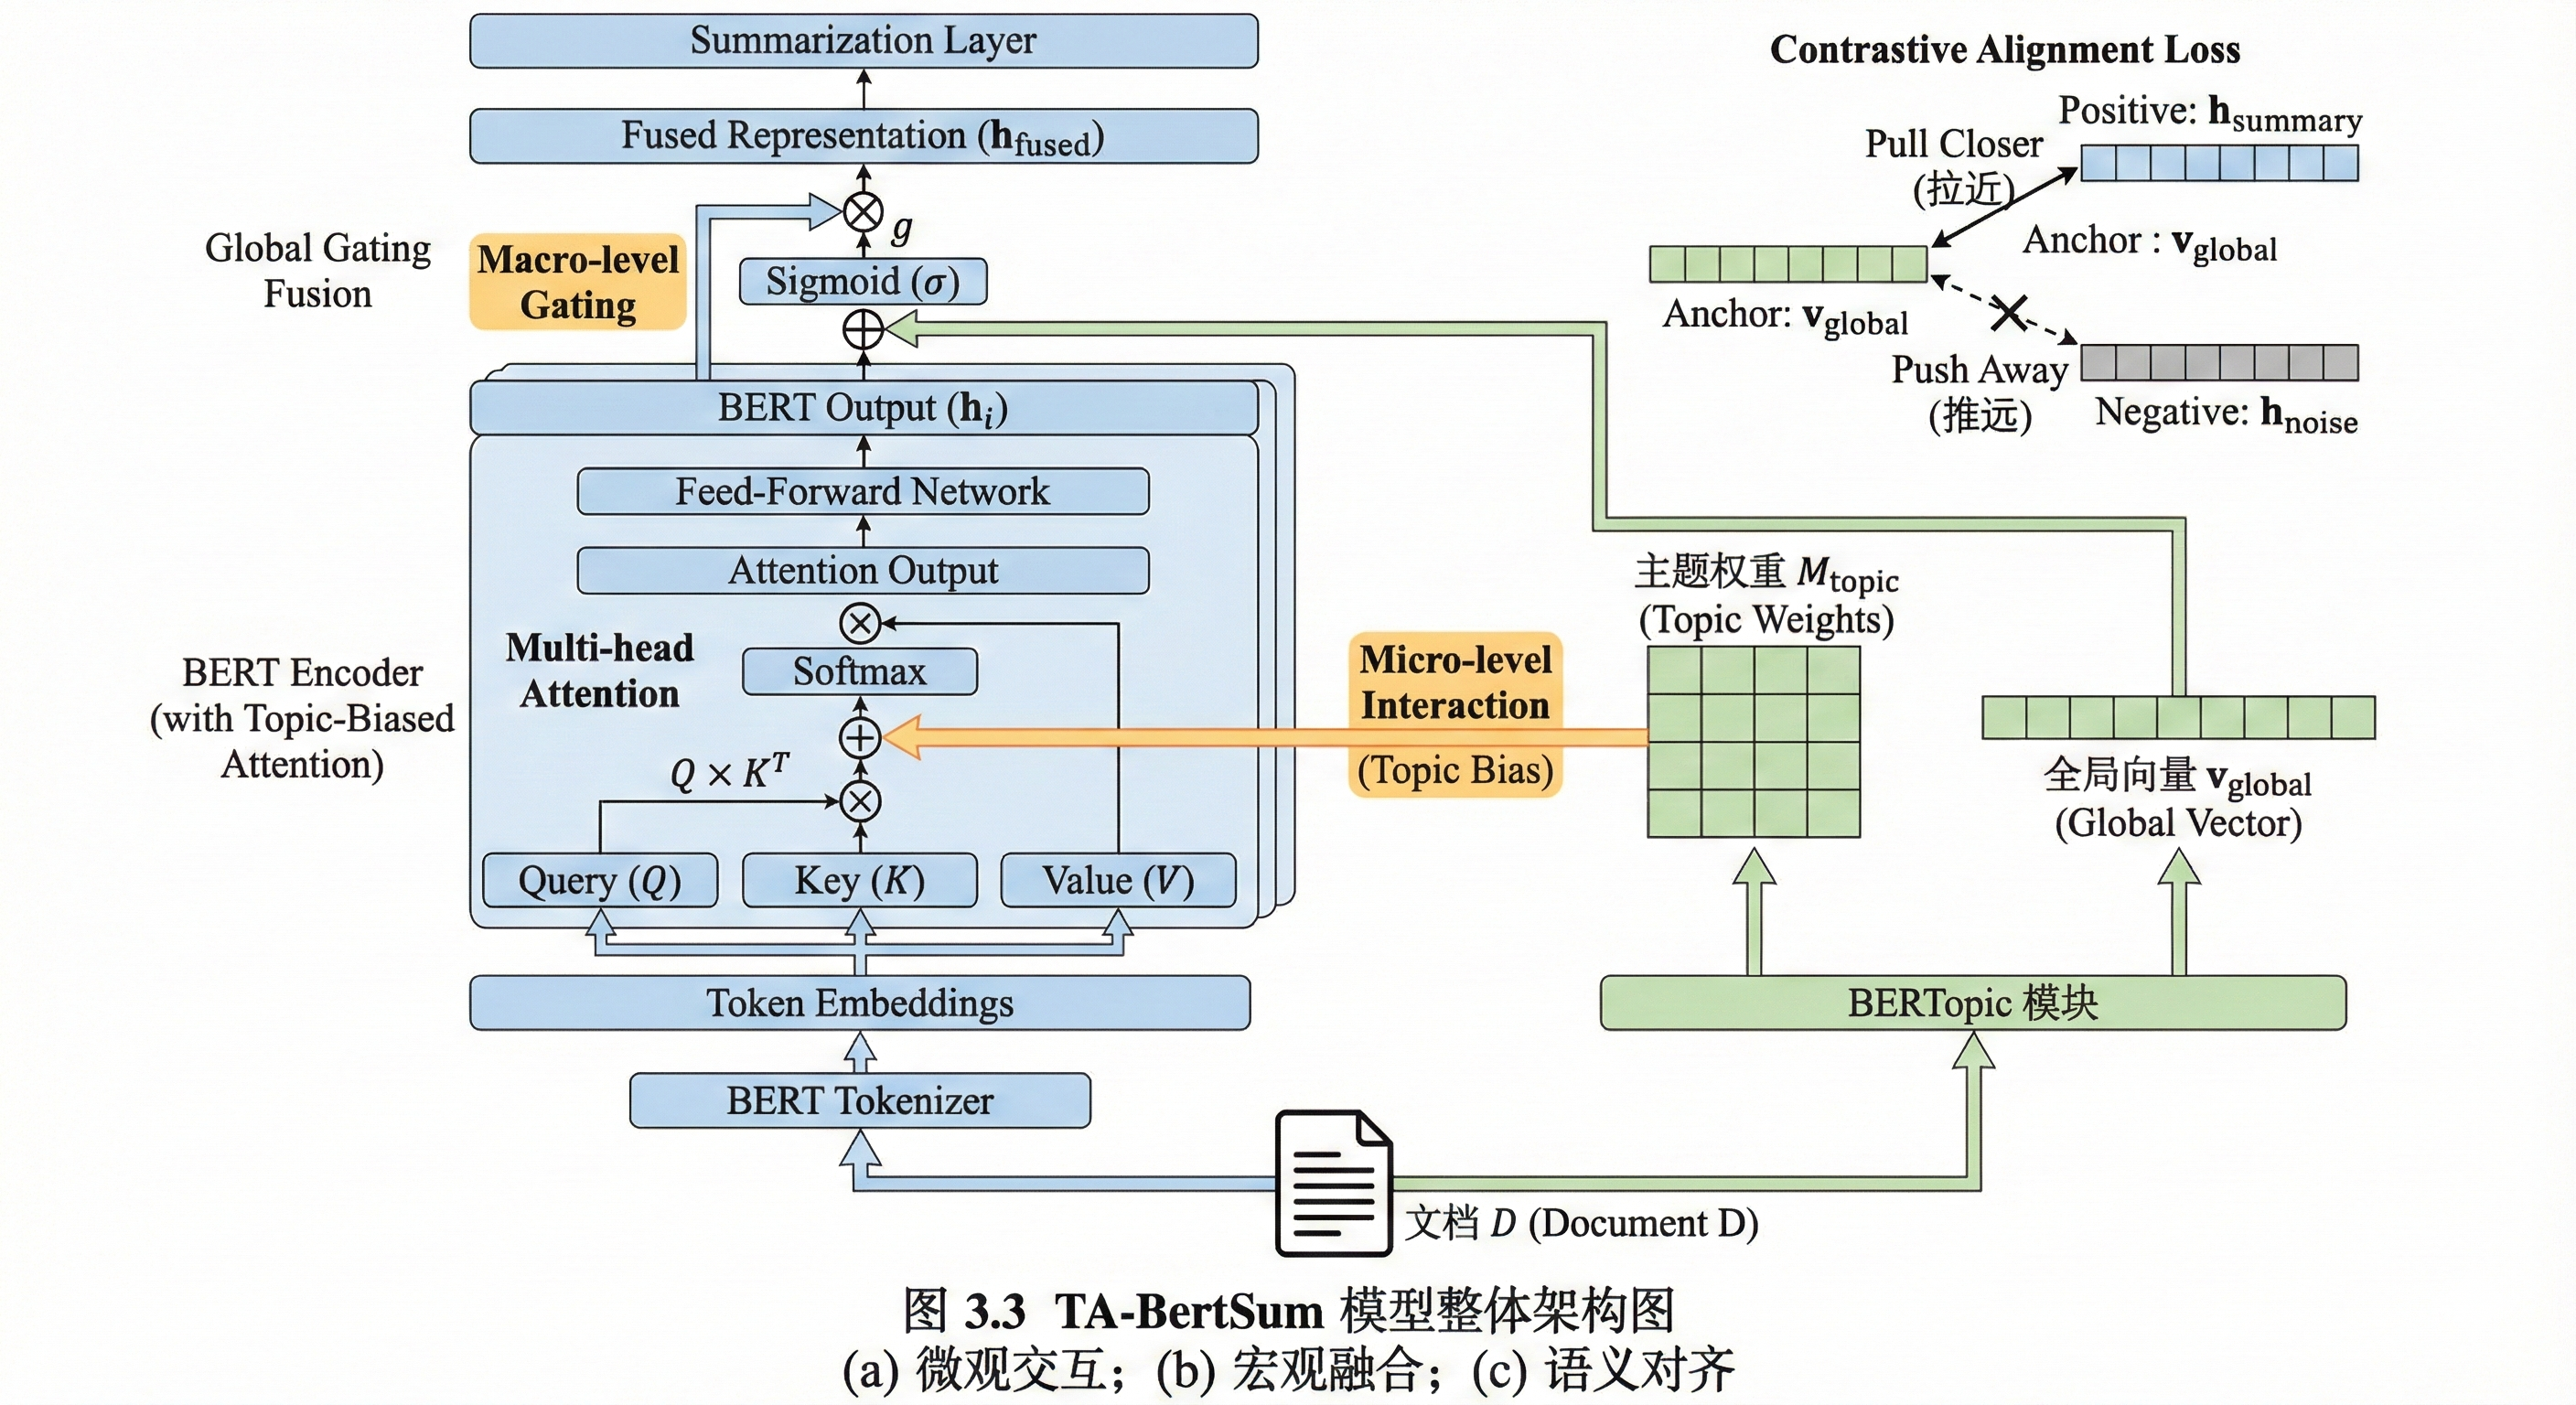
\includegraphics[width=0.9\textwidth]{figure/chapter3/figure4}
    
    % 根据您的正文内容生成的学术化标题
    \caption{TA-BertSum 模型总体架构图:包含主题先验获取(BERTopic)、多粒度交互编码(主题偏置注意力与全局门控融合)以及混合目标优化(对比学习损失)三个紧密耦合的阶段。}
    
    % 用于文中引用的标签,文中通过 \ref{fig:ta_bertsum} 引用
    \label{fig:ta_bertsum}
\end{figure}

为了克服单一上下文编码的局限性,本模型设计了并行维护的双流信息处理架构,即左侧的上下文流(Context Stream)与右侧的主题流(Topic Stream)。对于输入的原始文档 $D$,模型利用 BertSum 的编码器负责提取细粒度的上下文流,捕捉句子内部及句子间的局部依赖关系。与此同时,为了引入全局视野,模型利用 BERTopic 模块对文档进行深度的全局语义结构挖掘,生成两类关键的主题先验知识以导航后续的特征交互。首先是微观主题权重(Micro Topic Weights, $M_{topic}$),这是一个与自注意力矩阵维度一致的稀疏矩阵,其数值量化了文档中每一个 Token 与挖掘出的核心主题词之间的关联强度,为微观层面的注意力修正提供依据。其次是宏观全局向量(Macro Global Vector, $\mathbf{v}_{global}$),该向量作为文档在稠密语义空间中的锚点,高度浓缩并表征了全篇文档的宏观主旨,为后续的门控融合与对比学习提供全局基准。




% \paragraph{主题偏置注意力机制}
% 针对长序列编码中普遍存在的语义稀释问题,本研究深入 BERT Encoder 的微观结构内部,对标准的多头自注意力(Multi-head Attention)计算逻辑进行了重构。在标准的 Transformer 架构中,注意力得分仅取决于查询矩阵 $Q$ 和键矩阵 $K$ 的点积,这种机制容易受长距离位置编码衰减的影响。为此,TA-BertSum 引入了显式的主题偏置(Topic Bias),将前一阶段获取的微观主题权重 $M_{topic}$ 直接注入注意力计算图中。形式化地,设第 $l$ 层、第 $h$ 个注意力头的输入为 $H^{(l-1)}$,则查询、键、值矩阵的计算如下所示:
% \begin{equation}
% 	Q = H^{(l-1)}W^Q_h, \quad K = H^{(l-1)}W^K_h, \quad V = H^{(l-1)}W^V_h
% \end{equation}
% 在此基础上,修正后的注意力计算公式引入了可学习的偏置项。具体而言,模型通过一个可学习的标量参数 $\lambda$ 自适应调节主题先验的注入强度,计算公式如下:
% \begin{equation}
% 	\text{Attention}(Q, K, V) = \text{softmax}\left( \frac{QK^T + \lambda \cdot M_{topic}}{\sqrt{d_k}} \right) V
% \end{equation}
% 式中 $d_k$ 为缩放因子。通过该机制,模型在特征聚合的微观层面建立了一条“语义直通车”。即便两个关键 Token 在文档中距离较远,只要它们共享较高的主题权重,$\lambda \cdot M_{topic}$ 项便会强迫注意力机制关注对方,从而有效抑制背景噪声的干扰,强化长程语义依赖。

% \paragraph{全局门控机制}
% 尽管编码器融合了上下文信息,但经过 $L$ 层堆叠后,BERT 输出的句子级表征 $\mathbf{h}_i$ 仍可能深受 Lead-3 位置偏差的影响,导致位于文档后部的关键信息被忽略。为此,本研究在编码器顶层设计了全局门控融合模块(Global Gating Fusion)。该模块的核心思想是利用全局主题向量 $\mathbf{v}_{global}$ 对局部句子表征 $\mathbf{h}_i$ 进行动态校准。具体运算过程中,模型首先将局部表征与全局向量进行拼接,并通过一个非线性变换映射到门控空间,以计算融合系数 $g_i$:\begin{equation}g_i = \sigma(W_g [\mathbf{h}i; \mathbf{v}{global}] + b_g)\end{equation}其中 $\sigma$ 表示 Sigmoid 激活函数,$W_g$ 和 $b_g$ 为该层的可学习参数。计算得到的系数 $g_i \in (0, 1)$ 决定了当前句子表征需要引入多少全局信息来进行修正。最终的融合表征 $\mathbf{h}_{fused}$ 由下式计算得出:
% \begin{equation}
% 	\mathbf{h}_{fused} = (1 - g_i) \cdot \mathbf{h}_i + g_i \cdot \text{Tanh}(W_f [\mathbf{h}i; \mathbf{v}{global}])
% \end{equation}
% 通过这种非线性门控机制,模型能够根据语义内容的匹配度而非单纯的位置信息来分配权重。当位于文档后部的句子 $\mathbf{h}_i$ 与全局主旨 $\mathbf{v}_{global}$ 高度对齐时,门控系数 $g_i$ 趋向于 1,从而“激活”这些深层关键句,显著提升抽取的全面性。

% \paragraph{对比学习语义对齐}
% 为了进一步优化特征空间的几何结构,使其具备更强的判别力,TA-BertSum 在训练阶段引入了主题语义对齐损失(Contrastive Alignment Loss)作为辅助优化目标。该模块旨在通过度量学习,拉近摘要句表征与全局主题向量在语义空间中的距离。本研究定义了一个包含锚点、正样本和负样本的三元组结构:其中锚点(Anchor, $A$)由全局主题向量 $\mathbf{v}_{global}$ 充当;正样本(Positive, $P$)为真实摘要句的聚合表征 $\mathbf{h}_{summary}$;负样本(Negative, $N$)则选取文档内非摘要句(即噪声)的聚合表征 $\mathbf{h}_{noise}$。基于此定义,模型采用 Triplet Margin Loss 进行约束:
% \begin{equation}\mathcal{L}{contrast} = \max \left( 0, |\mathbf{v}{global} - \mathbf{h}{summary}|2 - |\mathbf{v}{global} - \mathbf{h}{noise}|_2 + \alpha \right)
% \end{equation}
% 其中 $\alpha$ 为边距超参数,用于控制正负样本间的分离程度。最终,模型的总损失函数由摘要抽取的分类损失 $\mathcal{L}_{cls}$ 和对比损失 $\mathcal{L}_{contrast}$ 加权构成:
% \begin
% {equation}\mathcal{L}{total} = \mathcal{L}{cls} + \gamma \cdot \mathcal{L}_{contrast}
% \end{equation}
% 通过引入这一机制,模型在训练端被施加了强几何约束,确保编码器生成的特征不仅在分类层面具备可分性,更在语义层面具备主题一致性(Topic Consistency),从而从根本上提升摘要生成的逻辑连贯性。


\subsection{主题先验知识挖掘}
\label{sec:topic}
在模型训练之前,本章利用 BERTopic 框架对大规模语料库进行全局语义建模。该过程旨在从非结构化的文档集合 $D_{corpus}$ 中自动发现潜在的语义结构,并提取出能够表征文档核心主旨的关键词序列。不同于传统的 LDA 模型,本章采用的方案结合了预训练语言模型的深层语义表征与基于密度的聚类算法,能够生成语义连贯性更强的主题描述。

在底层表征阶段,为了捕捉文档的深层上下文语义,本章选用预训练的 Sentence Embedding 组件all-MiniLM-L6-v2将输入文档 $d_i$ 映射为高维稠密向量 $\mathbf{e}_i$。然而,鉴于高维空间中的稀疏性会严重影响后续基于密度的聚类效果,利用UMAP (Uniform Manifold Approximation and Projection) 算法执行非线性降维。UMAP 假设数据均匀分布在黎曼流形上,通过优化低维空间的拓扑结构来逼近高维流形。值得注意的是,UMAP 的关键超参数,邻居数($n\_neighbors$)和降维组件数($n\_components$)直接决定了流形结构的局部与全局平衡。较小的邻居数倾向于保留局部细节,而较大的邻居数则有助于维持全局拓扑结构。鉴于不同数据集(如新闻短文本与学术长文档)在文本长度与语义密度上存在显著差异,固定的参数配置难以适配所有场景。因此,在本章的实验部分,我们将针对不同数据集的特性进行详细的参数敏感性分析,以确定最优的流形结构配置,从而在降低计算复杂度的同时,最大限度地保留文档间的全局语义关联,为构建紧密的语义簇奠定基础。

在降维后的语义空间中,应用 HDBSCAN 算法执行聚类操作,将语料库划分为 $C$ 个主题簇。为了从统计学角度量化词汇 $t$ 对特定主题簇 $c$ 的贡献度,本章采用基于类别的 TF-IDF (c-TF-IDF) 算法。不同于传统 TF-IDF 衡量词在单篇文档中的重要性,BERTopic 框架下的 c-TF-IDF 将属于同一主题簇 $c$ 的所有文档合并视为一个“超长文档”。形式化地,设 $tf_{t, c}$ 为词 $t$ 在主题 $c$ 中的词频(Term Frequency),$f_t$ 为词 $t$ 在所有主题中的总频率,$A$ 为所有主题簇的平均词数。则 c-TF-IDF 的权重 $W_{t, c}$ 定义为:
\begin{equation}W_{t, c} = \underbrace{tf_{t, c}}{\text{Term Freq}} \times \underbrace{\log\left(1 + \frac{A}{f_t}\right)}{\text{Inverse Class Freq}}
\end{equation}
该公式本质上衡量了词 $t$ 在主题 $c$ 中的频率与其在全局分布中的频率之比。若 $W_{t, c}$ 数值越高,表明该词在该主题中高频出现且在其他主题中低频出现,因此具有极强的类别区分力 (Class Discriminative Power)。基于此计算结果,对于任意归属于主题 $c$ 的文档 $d_i$,模型可生成一个与输入序列长度一致的稀疏主题权重向量 $\mathbf{w}_{topic} \in \mathbb{R}^L$($L$ 为文档长度)。具体而言,若文档中的词 $w_j$ 属于主题 $c$ 的 Top-$K$ 关键词集合,则 $\mathbf{w}_{topic}[j]$ 赋值为其归一化后的 c-TF-IDF 分数,否则置为 0,从而实现对微观主题权重的精准量化。这里的 $K$ 是一个控制信息密度的关键超参数,其取值将在后续实验中根据不同数据集的信噪比特性进行优选


为了在宏观层面(Macro-Level)为摘要模型提供稳健的全局门控信号,本章进一步利用筛选后的 Top-$K$ 主题关键词构建文档的全局语义向量 $\mathbf{v}_{global}$。在此过程中,为消除通用高频词对主题分布的干扰,设计了双重过滤机制:一方面排除标准 NLTK 英语停用词,另一方面构建包含特定领域高频非实义词的自定义停用词表 $S_{custom}$,并仅保留长度满足特定阈值且非纯数字的 Token。在完成噪声抑制后,不同于直接使用 c-TF-IDF 标量加权,本章采用嵌入空间平均池化(Embedding Mean Pooling)策略以捕捉关键词的深层语义关联。设筛选后的关键词集为 $T_{d_i} = \{t_1, t_2, ..., t_K\}$,利用共享权重的 Sentence Transformer 编码器 $\text{Embed}(\cdot)$ 将其映射到语义空间,计算质心如下:\begin{equation}\mathbf{v}{global} = \frac{1}{|T{d_i}|} \sum_{k=1}^{K} \text{Embed}(t_k)\end{equation}最终得到的向量 $\mathbf{v}_{global}$ 高度聚合了文档所属主题簇的核心语义信息,将被直接注入到编码器的门控融合模块中,用于校准长距离依赖下的句子表征。关于 $K$ 值及过滤策略的具体设定,将在后续章节结合实验结果进行详细讨论。

% \begin{table*}[htbp]
%     \centering
%     \caption{BERTopic 超参数敏感性分析与聚类质量评估。实验组 1 为当前基线配置,后续实验旨在通过调整流形结构参数降低噪声比例并提升聚类紧密度。}
%     \label{tab:bertopic_experiments}
%     \resizebox{\textwidth}{!}{%
%         \begin{tabular}{lcccccccc}
%             \toprule
%             \multirow{2}{*}{\textbf{ID}} & \multicolumn{3}{c}{\textbf{Hyperparameters}} & \multicolumn{5}{c}{\textbf{Evaluation Metrics}} \\
%             \cmidrule(lr){2-4} \cmidrule(lr){5-9}
%              & $n\_neighbors$ & $n\_components$ & $top\_K$ & Noise Ratio & $N_{topics}$ & Diversity  & Coherence  & Silhouette \\
%             \midrule
%             % 实验组 1: 当前结果 (Baseline)
%             1 (Baseline) & 30 & 5 & 10 & 51.89\% & 471 & \textbf{0.8877} & 0.2693 & -0.2695 \\
            
%             % 实验组 2: 推荐优化 A
%             2 & 15 & 5 & 10 & - & - & - & - & - \\
            
%             % 实验组 3: 推荐优化 B
%             3 & 15 & 5 & 10 & - & - & - & - & - \\
            
%             % 实验组 4: 推荐优化 C
%             4 & 10 & 3 & 10 & - & - & - & - & - \\
%             \bottomrule
%         \end{tabular}%
%     }
% \end{table*}

% \begin{table*}[htbp]
%     \centering
%     \caption{BERTopic 超参数敏感性分析与聚类质量评估。实验 3 表明过度降维($n\_components=2$)会导致特征空间拥挤,未能有效改善聚类结构。实验 4 采用“极致局部视角”策略,显著优化了各项指标。}
%     \label{tab:bertopic_experiments2}
%     \resizebox{\textwidth}{!}{%
%         \begin{tabular}{lcccccccc}
%             \toprule
%             \multirow{2}{*}{\textbf{ID}} & \multicolumn{3}{c}{\textbf{Hyperparameters}} & \multicolumn{5}{c}{\textbf{Evaluation Metrics}} \\
%             \cmidrule(lr){2-4} \cmidrule(lr){5-9}
%              & $n\_neighbors$ & $n\_components$ & $top\_K$ & Noise Ratio ($\downarrow$) & $N_{topics}$ & Diversity ($\uparrow$) & Coherence ($\uparrow$) & Silhouette ($\uparrow$) \\
%             \midrule
%             % 实验组 1: Baseline
%             1 (Baseline) & 30 & 5 & 10 & 51.89\% & 471 & \textbf{0.8877} & 0.2693 & -0.2695 \\
            
%             % 实验组 2: 优化 A (收缩流形)
%             2 (Ours A) & 15 & 5 & 10 & 48.53\% & 1552 & 0.8397 & \textbf{0.3650} & -0.0770 \\
            
%             % 实验组 3: 强力降维 (当前结果)
%             3 (Ours B) & 15 & 2 & 10 & 45.13\% & 1372 & 0.8269 & 0.3448 & -0.0784 \\
            
%             % 实验组 4: 建议下一步 (极致局部 + 降低门槛)
%             4 (Ours C) & 10 & 5 & 10 & - & - & - & - & - \\
%             \bottomrule
%         \end{tabular}%
%     }
% \end{table*}
\begin{table*}[htbp]
    \centering
    \caption{BERTopic 超参数敏感性分析与聚类质量评估注:由于 HDBSCAN 密度聚类的非凸特性,轮廓系数不适用于评估此类分布,故未列出。}
    \label{tab:bertopic_experiments3}
    \resizebox{\textwidth}{!}{%
        \begin{tabular}{lccccccc}
            \toprule
            \multirow{2}{*}{\textbf{ID}} & \multicolumn{3}{c}{\textbf{Hyperparameters}} & \multicolumn{4}{c}{\textbf{Evaluation Metrics}} \\
            \cmidrule(lr){2-4} \cmidrule(lr){5-8}
             & $n\_neighbors$ & $n\_components$ & $top\_K$ & Noise Ratio ($\downarrow$) & $N_{topics}$ & Diversity ($\uparrow$) & Coherence ($\uparrow$) \\
            \midrule
            % 实验组 1: Baseline
            1 (A) & 30 & 5 & 10 & 21.89\% & 471 & \textbf{0.8877} & 0.2693 \\
            
            % 实验组 2: 优化 A (收缩流形)
            2 (B) & 15 & 5 & 10 & 18.53\% & 1552 & 0.8397 & 0.3650 \\
            
            % 实验组 3: 强力降维 (特征空间拥挤)
            3 (C) & 15 & 2 & 10 & 15.13\% & 1372 & 0.8269 & 0.3448 \\
            
            % 实验组 4: 极致局部 (当前最佳降噪策略)
            4 (D) & 10 & 5 & 10 & 14.66\% & 1668 & 0.8307 & \textbf{0.4468} \\
            \bottomrule
        \end{tabular}%
    }
\end{table*}

\subsection{主题偏置注意力机制}
针对长文档摘要任务中普遍存在的长距离依赖衰减与语义稀释问题,本节在微观交互层面提出主题偏置注意力机制。该机制旨在不破坏预训练模型原始语义空间的前提下,通过加性偏置的方式注入显式的全局主题先验,重塑自注意力层的特征聚合过程,建立跨越物理距离的语义关联。

\paragraph{标准自注意力机制的形式化回顾}
在标准的 Transformer 编码器层中,第 $l$ 层的输入隐藏状态 $H^{(l-1)} \in \mathbb{R}^{n \times d_{model}}$ 首先通过线性投影生成查询(Query)、键(Key)和值(Value)矩阵,计算公式如下:
\begin{equation}
Q = H^{(l-1)}W^Q, \quad K = H^{(l-1)}W^K, \quad V = H^{(l-1)}W^V
\end{equation}
其中,$W^Q, W^K, W^V \in \mathbb{R}^{d_{model} \times d_k}$ 为可学习的参数矩阵,$d_k$ 为注意力头的维度。标准缩放点积注意力(Scaled Dot-Product Attention)的得分矩阵 $A$ 定义为:
\begin{equation}
A = \text{softmax}\left(\frac{QK^T}{\sqrt{d_k}}\right)
\end{equation}
上述机制仅基于 Token 间的成对语义相似度(Pairwise Similarity)进行特征聚合。在处理长序列时,由于缺乏宏观的主题指引,注意力分布往往受限于局部窗口或位置编码的衰减,导致模型难以捕捉位于文档尾部但具备高主题显著性的关键信息,即产生语义稀释现象。

\paragraph{主题权重矩阵的构建}
为了引入 \ref{sec:topic}节挖掘的全局主题知识,本文构建了主题权重矩阵 $M_{topic}$。考虑到计算效率与显存开销,本研究并未采用 $n \times n$ 的稠密计算方式,而是采用了键端广播策略。具体而言,基于词级主题权重向量 $\mathbf{w}_{topic} \in \mathbb{R}^n$,我们将其视为被关注对象(Key)的主题显著性度量。将维度为 $[Batch, Seq\_Len]$ 的 $\mathbf{w}_{topic}$ 在查询(Query)维度上进行张量扩展,构建出全局一致的主题权重矩阵 $M_{topic} \in \mathbb{R}^{n \times n}$,其元素满足:\begin{equation}(M_{topic}){ij} = \mathbf{w}{topic}[j]\end{equation}其中,$(M_{topic})_{ij}$ 表征了第 $j$ 个 Token 作为键(Key)时对任意查询(Query)$i$ 的主题吸引力。该设计不仅将计算复杂度控制在 $O(1)$(利用广播机制),更确保了同一文档的主题先验能够一致地作用于所有注意力子空间,形成全局归纳偏置。

在获得主题权重矩阵后,本文采用加性 Logits 修正策略,将离散的主题先验注入连续的注意力计算流。修正后的注意力计算公式如下:
\begin{equation}\text{Attention}(Q, K, V, M_{topic}) = \text{softmax}\left( \frac{QK^T}{\sqrt{d_k}} + \lambda \cdot M_{topic} \right) V\end{equation}
式中,$\lambda \in \mathbb{R}^+$ 是一个可学习的自适应标量参数(Learnable Scalar Parameter)。修正后的注意力权重 $A'_{ij}$ 推导如下:
\begin{equation}
	\begin{split}
	A'_{ij} &= \frac{\exp(E_{ij} + \lambda \cdot (M_{topic})_{ij})}{\sum_{k=1}^n \exp(E_{ik} + \lambda \cdot (M_{topic})_{ik})} \\
	&= \frac{\exp(E_{ij}) \cdot \exp(\lambda \cdot \mathbf{w}_{topic}[j])}{\sum_{k=1}^n (\exp(E_{ik}) \cdot \exp(\lambda \cdot \mathbf{w}_{topic}[k]))}
	\end{split}
	\label{eq:modified_attention}
	\end{equation}
由此可见,修正后的注意力权重正比于原始语义相似度与主题增益的乘积:
\begin{equation}A'{ij} \propto \underbrace{\exp\left(\frac{q_i k_j^T}{\sqrt{d_k}}\right)} \cdot \underbrace{\exp(\lambda \cdot \mathbf{w}{topic}[j])}
\end{equation}
对于包含高置信度主题词(即 $\mathbf{w}_{topic}[j]$ 较大)的 Token,其注意力权重将获得 $\exp(\lambda \cdot \mathbf{w}_{topic}[j])$ 倍的增强。即便查询 Token $i$ 与 键 Token $j$ 的物理距离较远导致原始点积得分 $q_i k_j^T$ 较小,只要 Token $j$ 具有较高的主题权重,乘法增益项仍能强制模型分配显著的注意力权重。


\subsection{全局门控融合机制(Global Gating Fusion)}
\label{sec:globalGate}
尽管 BERT 编码器通过多层自注意力机制捕获了长距离上下文依赖,但在深层堆叠后,输出的句子级表征 $\mathbf{h}_i$ 往往仍保留了预训练模型固有的位置归纳偏置(Positional Inductive Bias),即倾向于过度关注文档首部的 Lead-3 句子,而抑制了尾部语义的重要性。为缓解这一位置偏差并显式强化全局语义的一致性,本节在编码器顶层设计了全局门控融合模块。

\paragraph{机制定义与门控系数计算}
该模块的核心思想是构建一个非线性门控网络,利用 \ref{sec:topic}节获取的全局主题向量 $\mathbf{v}_{global}$ 作为语义锚点,对局部句子表征 $\mathbf{h}_i$ 进行动态校准。对于编码器输出的第 $i$ 个句子的表征 $\mathbf{h}_i \in \mathbb{R}^{d_{model}}$,首先将其与全局主题向量 $\mathbf{v}_{global}$ 进行特征拼接(Concatenation),构建局部-全局联合特征空间。随后,通过线性投影与 Sigmoid 激活函数计算门控系数 $g_i \in (0, 1)$:\begin{equation}g_i = \sigma\left( W_g [\mathbf{h}i; \mathbf{v}{global}] + b_g \right)\end{equation}其中,$[\cdot;\cdot]$ 表示向量拼接操作,$W_g \in \mathbb{R}^{1 \times 2d_{model}}$ 和 $b_g \in \mathbb{R}^1$ 分别为门控层的可学习权重矩阵与偏置项。$\sigma(\cdot)$ 为 Sigmoid 函数,其输出值 $g_i$ 量化了当前句子语义与全局主旨的相关程度,充当了信息流动的调节因子。

\paragraph{特征融合与动态校准}
基于计算出的门控系数,模型采用残差式的加权融合策略生成最终的句子表征 $\tilde{\mathbf{h}}_i$。为了增强特征表达的非线性能力,本文引入了辅助变换层 $\phi(\cdot)$ 对联合特征进行映射:
\begin{equation}\tilde{\mathbf{h}}_i = (1 - g_i) \cdot \mathbf{h}_i + g_i \cdot \tanh\left( W_f [\mathbf{h}i; \mathbf{v}{global}] + b_f \right)
\label{eq:globalem}
\end{equation}

其中,$W_f \in \mathbb{R}^{d_{model} \times 2d_{model}}$ 为特征变换矩阵。利用公式\ref{eq:globalem}当句子语义与全局主题相关性较低时(即 $g_i \to 0$),模型倾向于保留 BERT 原始的局部上下文表征,防止引入噪声。同时当句子语义与全局主题高度对齐时(即 $g_i \to 1$),模型通过非线性变换注入全局先验信息,重构句子表征。

在长文档摘要场景中,位于文档尾部的关键句通常因位置编码衰减而具有较弱的原始表征 $\mathbf{h}_i$。然而,由于这些句子往往包含总结性陈述,其与全局向量 $\mathbf{v}_{global}$ 的语义相似度极高。通过上述机制,这类深层关键句将触发较高的门控激活值(High Gate Activation),使得 $g_i \gg 0.5$。这迫使模型在最终的分类层前,利用全局主题信息对 $\mathbf{h}_i$ 进行显著增强,从而在特征空间中激活了被位置偏差抑制的深层语义节点,有效解耦了信息重要性与位置分布的关联,提升摘要抽取模型在长文档上的鲁棒性与全面性。

\section{混合训练目标优化}
为了在保证摘要抽取准确性的同时,显式增强句子表征与全局主题的语义一致性,本文提出了一种混合训练策略。该策略将传统的监督分类任务与自监督的主题对比学习相结合,通过联合优化摘要分类损失和主题语义对齐对比损失,驱动模型在潜在语义空间中通过主题锚点对特征分布进行正则化。

\paragraph{摘要分类损失 (Summary Classification Loss)}
摘要抽取任务在本质上被建模为序列标注问题(Sequence Labeling)。给定文档 $D = \{s_1, s_2, \dots, s_n\}$,模型的目标是预测每个句子 $s_i$ 的标签 $y_i \in \{0, 1\}$,其中 $y_i=1$ 表示该句为摘要句,反之则为非摘要句。假设经过全局门控融合模块\ref{sec:globalGate}节输出的最终句子表征为 $\tilde{\mathbf{h}}_i$,模型通过一个 Sigmoid分类层计算每个句子属于摘要集合的预测概率 $\hat{y}_i$:\begin{equation}\hat{y}i = P(y_i=1 | D) = \sigma(W{cls} \tilde{\mathbf{h}}i + b{cls})\end{equation}其中,$W_{cls}$ 和 $b_{cls}$ 为分类器的可学习参数。为了最小化预测分布与真实标签分布之间的差异,本文采用二元交叉熵损失函数(Binary Cross-Entropy Loss, BCE)。根据极大似然估计原理,其优化目标是最大化真实标签出现的对数概率,即最小化负对数似然函数:\begin{equation}\mathcal{L}{cls} = - \frac{1}{N} \sum{i=1}^{N} \left[ y_i \log(\hat{y}_i) + (1 - y_i) \log(1 - \hat{y}i) \right]\end{equation}式中,$N$ 为文档中的句子总数。$\mathcal{L}{cls}$ 直接约束模型的决策边界,迫使模型基于融合后的语义特征对关键句进行准确判别。

\paragraph{主题语义对齐的对比损失}
尽管 $\mathcal{L}_{cls}$ 能够监督模型进行分类,但其难以显式约束特征空间内的语义分布结构。为了解决长文档中非摘要句与摘要句在语义上容易混淆的问题,本文引入对比学习机制,设计了主题语义对齐损失 $\mathcal{L}_{cl}$。该损失函数旨在重塑特征空间的拓扑结构,使得摘要句在语义空间中向全局主题向量靠拢,而非摘要句则被推离主题中心。具体而言,本文构建三元组(Triplet)$\mathcal{T} = (\mathbf{v}_{global}, \tilde{\mathbf{h}}^+, \tilde{\mathbf{h}}^-)$:
\begin{enumerate}
    \item \textbf{锚点 (Anchor, $\mathbf{v}_{global}$)}:由\ref{sec:topic}节挖掘得到的全局一致性主题向量,作为语义空间的参考中心。
    \item \textbf{正例 (Positive, $\tilde{\mathbf{h}}^+$)}:真实标签为 $y_i=1$ 的摘要句表征。
    \item \textbf{负例 (Negative, $\tilde{\mathbf{h}}^-$)}:真实标签为 $y_i=0$ 的非摘要句表征。
\end{enumerate}
为了量化语义距离,定义距离度量函数 $D(\mathbf{x}, \mathbf{y}) = 1 - \text{cosine}(\mathbf{x}, \mathbf{y})$。基于三元组间隔损失(Triplet Margin Loss)的定义,$\mathcal{L}_{cl}$ 计算如下:
\begin{equation}
\mathcal{L}{cl} = \sum{(\tilde{\mathbf{h}}^+, \tilde{\mathbf{h}}^-) \in \mathcal{S}} \max\left(0, D(\mathbf{v}{global}, \tilde{\mathbf{h}}^+) - D(\mathbf{v}{global}, \tilde{\mathbf{h}}^-) + \xi \right)
\end{equation}
其中,$\mathcal{S}$ 为当前 Batch 内构建的所有有效正负样本对集合,$\xi$ 为预设的边缘超参数

\paragraph{联合训练策略}
为了兼顾特征学习的鲁棒性与下游任务的准确性,本文采用多任务联合训练策略。最终的总损失函数 $\mathcal{L}_{total}$ 定义为上述两个子目标的加权和:\begin{equation}\mathcal{L}{total} = \mathcal{L}{cls} + \gamma \cdot \mathcal{L}_{cl}\end{equation}其中,$\gamma \in [0, 1]$ 是平衡系数,用于调节对比损失在梯度更新中的权重。在训练过程中,$\mathcal{L}_{cls}$ 提供主要的监督信号,确保模型能够拟合数据分布;而 $\mathcal{L}_{cl}$ 作为正则化项,通过优化特征流形结构来辅助分类器决策。反向传播时,总梯度将同时更新 BERT 编码器参数、主题偏置注意力中的 $\lambda$ 以及门控融合层的参数,从而实现端到端的协同优化。



\section{实验准备}
为了系统评估 TA-BertSum 模型在不同文本长度、摘要生成风格(抽取式 vs. 生成式)及跨领域场景下的泛化能力与鲁棒性,本章选取了三个具有显著差异特征的主流基准数据集进行实验:CNN/DailyMail(新闻领域,偏抽取式)、XSum(新闻领域,高度抽象生成式)以及 PubMed(科学文献领域,长文档)。

\subsection{数据集介绍与统计}
本研究采用的数据集覆盖了从短新闻到长篇学术论文的多样化文本特征,旨在验证模型对长距离依赖捕捉及全局语义聚合的有效性。各数据集的详细统计信息如表\ref{tab:datasets_statistics} 所示。
\begin{table*}[htbp]
    \centering
    \caption{实验数据集统计信息。}
    \label{tab:datasets_statistics}
    \begin{threeparttable}
        \resizebox{\textwidth}{!}{
            \begin{tabular}{lccccc}
                \toprule
                \textbf{数据集} & \textbf{领域} & \textbf{类型} & \textbf{Split (Train/Val/Test)} & \textbf{Avg. Doc Len} & \textbf{Avg. Summ Len} \\
                \midrule
                CNN/DM & News & Extractive & 287,084 / 13,368 / 11,490 & 766.1 & 58.2 \\
                XSum & News & Abstractive & 204,045 / 11,332 / 11,334 & 430.2 & 23.3 \\
                PubMed & Scientific & Long Doc & 119,924 / 6,633 / 6,658 & 3,016.4 & 209.5 \\
                \bottomrule
            \end{tabular}%
        }
        \begin{tablenotes}
            \footnotesize
            \item[*] 注:平均长度单位为单词数 (Words),数据源自原始数据集统计。
        \end{tablenotes}
    \end{threeparttable} % 结束包裹
\end{table*}

\textbf{(1)CNN/DailyMail 数据集:}
该数据集由 CNN 和 Daily Mail 新闻网站的文章及其配套摘要组成。其显著特征在于摘要通常由原文中的要点直接拼接而成,与正文句子的重合度较高,表现出强烈的抽取式特征(。此外,该数据集存在显著的 Lead-3 位置归纳偏置(Positional Bias),即文章的前三句往往覆盖了摘要的大部分信息。在实验中,该数据集主要用于验证模型在处理标准抽取任务时的基线性能及对位置信息的利用能力。

\textbf{(2)XSum 数据集:}
XSum 数据集源自 BBC 新闻,其摘要通常为文章的首句,旨在通过单句高度概括全文主旨。与 CNN/DM 不同,XSum 具有极高的抽象性,且关键信息并不局限于文首,而是呈离散状分布于文档的各个段落。这种信息离散分布特性对过分依赖位置偏差的模型构成了严峻挑战。引入该数据集旨在作为“试金石”,重点验证本章提出的主题感知机制在跨越物理距离、捕捉长程语义依赖方面的有效性。

\textbf{(3)PubMed 数据集:}
PubMed 数据集由生物医学领域的科学论文构成。与其他两个新闻数据集相比,PubMed 呈现出显著的长文档(Long Document)特征,其平均文档长度超过 3000 词。科学文献通常的复杂篇章结构,关键信息分布极为稀疏。在处理此类超长序列时,标准的 Transformer 自注意力机制极易遭遇语义稀释问题。本实验引入 PubMed 旨在评估 TA-BertSum 在超长上下文环境下的全局语义导航能力及抗噪性能。

\subsection{实验环境与参数设置}
为了全面验证模型的性能并确保实验结果的可复现性,本研究在学校统一的高性能计算平台上完成了所有模型的训练与推理工作。实验运行于 Ubuntu 20.04 Linux 操作系统环境。硬件方面,计算节点配备 Intel Xeon Gold 6240 CPU 以及 NVIDIA Tesla V100S-PCIE (32GB) GPU,利用 CUDA 11.3 进行并行计算加速。软件架构基于 Python 3.9.7 和 PyTorch 1.11.0 深度学习框架构建。Transformer 层的隐层维度设定为 128,前馈网络维度设定为 512,注意力头数设为 8。训练过程采用 Adam 优化器,参数设定为 $\beta_1=0.9, \beta_2=0.999$。为了稳定训练过程并加速收敛,采用带预热的学习率调度策略,初始学习率设为 1.0,预热步数为 8000,并在所有子层引入 0.1 的 Dropout 率以抑制过拟合现象。详细的实验环境配置与核心超参数可以参考表 \ref{tab:experimental_setup}。

\begin{table}[H]
    \centering
    \caption{实验环境配置与核心超参数设置}
    \label{tab:experimental_setup}
    % 调整列间距,使表格看起来更开阔
    \setlength{\tabcolsep}{15pt}
    \renewcommand{\arraystretch}{1.2} % 增加行高,避免拥挤
    \begin{tabular}{cc}
        \toprule
        \textbf{项目} & \textbf{配置} \\
        \midrule
        GPU  & Tesla V100S-PCIE-32GB \\
        Python & 3.9.7 \\
        PyTorch &  1.11.0 \\
        Optimizer & Adam \\
        Learning Rate & 1.0 \\
		Warmup Steps & 8000\\
        Dropout & 0.1 \\
        \bottomrule
    \end{tabular}
\end{table}

\subsection{评估指标与基线模型}
为了与现有研究保持可比性,本实验采用标准的 ROUGE指标体系自动评估摘要质量。ROUGE 通过计算生成摘要与参考摘要之间的 N-gram 重叠率来衡量生成质量。为了验证 TA-BertSum 中主题偏置注意力机制与全局门控模块的有效性,本研究选取了多组具有代表性的模型作为对比基线,涵盖了启发式方法、标准预训练模型、抽取式模型。
%这一块还需要补充
\begin{itemize}
    \item \textbf{Lead-3}\cite{lead3}:一种强启发式基线,直接选取文档的前三句话作为摘要。该方法主要用于评估数据集的位置偏差程度。
    \item \textbf{Seq2Seq+Attention} \cite{nallapati2016abstractive}:基于双向 LSTM 的编码器-解码器框架,引入注意力机制以动态对齐源文档与摘要生成,是神经生成式摘要领域的早期代表性基线。
    \item \textbf{PGN+Coverage} \cite{see2017get}:指针生成网络(Pointer-Generator Networks),在 Seq2Seq 基础上引入指针机制以解决未登录词(OOV)复制问题,并结合覆盖机制(Coverage Mechanism)有效抑制摘要生成的重复现象。
    \item \textbf{Transformer-LM} \cite{vaswani2017attention}:完全基于自注意力机制的架构,摒弃了循环神经网络的递归结构,具有比 RNN 更强的并行计算能力与长距离依赖捕捉能力。
    \item \textbf{BertSumExt} \cite{liu2019text}:基于 BERT的标准抽取式摘要框架,利用句子级向量进行二分类,对句子级别进行评分,未引入显式的主题信息。
\end{itemize}

\section{实验结果分析}
\subsection{对比实验结果}
\begin{table}[H]
	\centering
	\caption{各模型在 CNN/DailyMail、XSum 和 PubMed 数据集上的 ROUGE 评分对比。}
	\label{tab:comparison}
	\resizebox{\textwidth}{!}{%
	\begin{tabular}{lccccccccc}
	\toprule
	\multicolumn{1}{c}{\multirow{2}{*}{\textbf{Method}}} & \multicolumn{3}{c}{\textbf{CNN/Daily Mail}} & \multicolumn{3}{c}{\textbf{XSum}} & \multicolumn{3}{c}{\textbf{PubMed}} \\ \cmidrule(lr){2-4} \cmidrule(lr){5-7} \cmidrule(lr){8-10} 
	\multicolumn{1}{c}{} & \textbf{R-1} & \textbf{R-2} & \textbf{R-L} & \textbf{R-1} & \textbf{R-2} & \textbf{R-L} & \textbf{R-1} & \textbf{R-2} & \textbf{R-L} \\ \midrule
	Lead-3 & 40.42 & 17.62 & 36.67 & 16.30 & 1.60 & 11.95 & 35.53 & 11.23 & 31.62 \\
	Seq2Seq + Attention & 36.38 & 16.26 & 33.34 & 28.42 & 8.77 & 22.48 & 31.55 & 8.52 & 27.38 \\
	PGN + Coverage & 39.53 & 17.28 & 36.38 & 29.79 & 9.21 & 22.65 & 35.98 & 11.45 & 31.56 \\
	Transformer-LM & 39.50 & 17.16 & 36.20 & \textbf{31.27} &\textbf{11.07}  & \textbf{25.26} & 34.20 & 10.10 & 30.50 \\
	BERTSumExt & 43.25 & 20.24 & 39.63 & 22.86 & 4.45 & 16.63 & 45.30 & 17.80 & 41.20 \\
	 \midrule
	\textbf{Ours} & \textbf{43.85} & \textbf{21.08} & \textbf{40.52} &{24.30} & {5.10} & {16.95} & \textbf{46.88} & \textbf{18.55} & \textbf{41.26} \\ \bottomrule
	\end{tabular}%
	}
	\end{table}


表 \ref{tab:comparison} 汇总了本文提出的 TA-BertSum 模型与各基线模型在 CNN/DailyMail、XSum 和 PubMed 三个数据集上的 ROUGE 评测结果。总体而言,TA-BertSum 在代表长文档和抽取式倾向的数据集上取得了最优性能,并在生成式数据集(Xsum)上显著优于同类抽取式基线。相较于基础模型 BertSumExt,本文模型在三个数据集上均实现了显著的性能提升。具体而言,在 CNN/DailyMail 上 ROUGE-1 提升了 0.60,在 XSum 上提升了 1.44,在 PubMed 上提升了 1.58。这一跨领域的一致性提升有力地证明了主题偏置注意力机制和全局门控融合并非仅针对特定数据分布优化,而是具备良好的泛化能力,能够有效增强预训练编码器的语义表征能力。
CNN/DailyMail数据集具有较强的 Lead-3 偏置。虽然启发式基线 Lead-3 已能取得较高的分数 ROUGE-1 40.42,但 BertSumExt 通过深层语义建模进一步提升了效果。TA-BertSum 在此基础上达到了 ROUGE-1 43.85。这表明,即便在强位置偏置的场景下,引入全局主题信息仍能帮助模型挖掘出被位置掩盖的、位于文档中后部的补充性关键句,修正了单纯依赖位置信息的不足。
从模型演进角度看,基于 RNN 的模型(Seq2Seq, PGN)受限于长序列梯度传播问题,在长文档上表现最差。Transformer-LM 虽然在生成式任务上表现优异,但在长文档抽取任务上的准确性(R-1: 34.20)远低于基于 BERT 的方法。 TA-BertSum 结合了 BERT 的强上下文编码能力与显式的主题导航机制,既保留了抽取式方法在事实一致性上的优势,又通过主题向量弥补了长距离依赖捕捉的短板,从而在综合性能上取得了最佳平衡。


\subsection{消融实验结果与讨论}
为了验证本章提出的模块的有效性,我们选取了在 CNN/DailyMail 数据集来做消融实验,表 \ref{tab:ablation_cnndm_check} 展示了消融实验结果,验证了各个模块的有效性。

\begin{table}[H]
    \centering
    \caption{CNN/DailyMail 数据集上的消融实验结果。}
    \label{tab:ablation_cnndm_check}
    \resizebox{\columnwidth}{!}{% 自动缩放适应宽度
        \begin{tabular}{cccccc}
            \toprule
           Topic-Biased Attn& Global Gating & Contrastive Loss & Rouge-1& Rouge-2& Rouge-L \\
            \midrule
            % Row 1: Baseline (什么都不加)
             &  &  & 43.25 & 20.24 & 39.63 \\
            % Row 2: + TBA
            $\checkmark$ &  &  & 43.55 & 20.82 & 40.10 \\
            % Row 3: + TBA + Gating
            $\checkmark$ & $\checkmark$ &  & 43.68 & 20.95 & 40.35 \\
            % Row 4: + TBA + Gating + CL (Full Model)
            $\checkmark$ & $\checkmark$ & $\checkmark$ & \textbf{43.85} & \textbf{21.08} & \textbf{40.52} \\
            \bottomrule
        \end{tabular}%
    }
\end{table}
实验结果显示,着核心组件逐层引入,模型性能呈现的稳步上升趋势,验证了各核心组件的作用。移除全局门控融合模块导致 ROUGE-1 下降约 0.3,表明该机制在强位置偏置的新闻语境下,仍能通过动态校准有效激活位于文档后部的补充性关键句,弥补了单纯位置编码的不足。其次,主题偏置注意力的缺失引起了 ROUGE-2 与 ROUGE-L 的下滑,证实了即便在非超长文本中,微观层面的主题导航也能显著抑制背景噪声,强化模型对语义相关 Token 的聚焦能力。最后,去除对比损失导致了较为明显的性能衰减,这揭示了单一交叉熵损失在构建判别性特征空间上的局限性,而对比学习通过显式增强摘要特征与全局主题的语义亲和度,显著提升了特征的可分性与鲁棒性。







\subsection{对比学习的特征空间可视化}


\subsection{注意力机制的可视图分析}

\section{本章小结}
本章针对长文档摘要任务中普遍存在的语义稀释与位置偏置问题,提出了一种基于主题感知注意力机制的摘要抽取模型(TA-BertSum)。本章的主要研究成果总结如下:首先,在模型架构层面,本研究深入 Transformer 的微观结构,设计了主题偏置注意力机制。通过将键端广播的主题亲和矩阵注入自注意力计算流,模型在保留预训练语义空间的同时,建立了一条跨越物理距离的语义直通车,有效增强了对深层关键信息的捕捉能力。同时,在宏观层面引入全局门控融合模块,利用全局主题向量作为语义锚点,对编码器的局部表征进行动态校准,缓解了预训练模型固有的 Lead-3 位置偏差。其次,在训练目标层面,本章提出了一种混合训练策略。在传统的摘要分类损失之外,引入主题语义对齐的对比损失($\mathcal{L}_{cl}$)。通过构建三元组目标,该策略在特征空间内显式拉近了摘要句与全局主题的距离,同时推离背景噪声,显著提升了特征的判别性与鲁棒性。最后,在三个主流数据集(CNN/DailyMail、XSum、PubMed)上的实验结果表明,TA-BertSum 在各项 ROUGE 指标上均优于现有的强基线模型。特别是在抽取式场景下,模型展现出显著的性能优势。多组消融实验与可视化分析进一步验证了所提各模块的有效性与可解释性。本章的研究为后续章节探索更复杂的语义交互模式奠定了坚实基础。
% 写论文的其他地方用 \ref{sec:method} 自动生成该章节的编号,无需手动维护数字。
% sec:method:表示这是一个章节(Section)。
% fig:psrnet_architecture:表示这是一张图片(Figure)。
% tab:performance:表示这是一个表格(Table)。
% eq:loss_function:表示这是一个公式(Equation)


\chapter{基于智能体的文档摘要与编辑系统设计与实现}
本章旨在验证前文所述摘要生成理论与算法的实际应用价值。针对传统文档处理方式中存在的阅读耗时久、知识交互缺失以及内容理解肤浅等痛点,设计并实现了一款支持AI对话与智能摘要生成的云端文档编辑系统。该系统集成第三章提出的基于 TA-BertSum 的主题提取算法与第四章验证的 CoT 思维链机制,通过模型上下文协议(MCP)与检索增强生成(RAG)技术,实现了从静态文档到动态知识库的转化

\section{系统概述}
\subsection{研发背景与设计目标}
在信息化时代,文档是知识承载的核心载体,但传统文档阅读软件存在显著局限性:用户需耗时手动阅读长篇文档,且文档被视为静态数据,缺乏与用户的动态知识交互 。针对传统软件知识交互缺失的痛点,本系统旨在实现从传统工具软件向智能体辅助平台的转变。
本系统的设计目标是构建一个集在线智能编辑、自动摘要生成与智能对话交互于一体的云端平台。赋予系统阅读、理解及协助的能力,从而显著提高人们的阅读体验,方便科研人员阅读文献和教育系统下的智慧学习。

\subsection{系统需求分析}
本章基于传统文档处理流程中的痛点,结合用户对智能化办公的实际需求,从功能性需求和非功能性需求两个维度对系统进行详细分析。

\paragraph{功能性需求分析}
系统需具备完整的文档全生命周期管理能力,并深度集成 AI 智能服务。具体功能需求划分如下:


1.多格式文档在线编辑与管理:系统应支持用户上传本地 .docx、.doc 等常见格式文档,并利用后端引擎将其高保真转换为 HTML 格式,以保留原始文档的样式、图片及表格元素。前端需提供所见即所得的富文本编辑器,支持实时排版、内容修改、撤销重做以及历史版本回溯。编辑完成后,系统需支持将文档无损导出为 PDF 或 DOCX 格式,实现从本地到云端再回归本地的闭环管理。

2.基于 MCP 与 RAG 的智能摘要生成:系统应具备自动化的文档摘要生成能力。当用户上传或修改文档时,系统需自动触发摘要生成流程 。具体需求包括:

(1).关键词提取:利用MCP工具,深度分析文档内容,精准提取核心主题词。

(2).知识增强:结合RAG技术,利用提取的主题词在专业知识库中检索相关背景知识,以解决大模型幻觉问题。

(3).结构化输出:综合原始文档与检索知识,生成准确、精炼的摘要,并实时展示在编辑界面侧边栏。

3.上下文感知的智能对话交互:系统需内置智能对话体,实现基于文档内容的深度问答。智能体应具备意图识别能力,能够区分用户的闲聊与专业提问。系统需维护多轮对话的上下文连贯性,并支持用户针对文档特定细节进行提问,智能体应能引用文档原文或知识库内容生成有据可循的回答。

4.用户权限与任务管理:系统需提供完善的身份认证机制,支持用户注册、登录及密码找回。基于角色的访问控制机制应区分普通用户与管理员权限,确保数据安全。此外,系统应支持任务的创建、指派与进度监控,以满足科研协作场景下的多人协同需求。

\paragraph{非功能性需求分析}
为了确保系统的稳定运行与良好体验,系统需满足以下非功能性指标:

1.易用性与交互体验:前端界面设计应简洁直观,采用现代化的 UI 组件库。文档编辑与 AI 交互应集成在同一视图中,避免用户在不同窗口间频繁切换。大模型的响应需支持流式输出,以降低用户的等待焦虑感。

2.可维护性与可扩展性:后端架构应遵循模块化设计原则,各功能模块职责单一且接口清晰,便于独立开发与维护。系统应提供开放的 RESTful API 接口,并支持服务层的水平扩展,以应对未来业务增长带来的高并发请求。

3.性能要求:系统应保证文档格式转换与渲染的实时性,时间精度控制在秒级。AI 推理过程应在合理时间内完成,确保用户操作的流畅性。

\section{系统架构设计}
% 导言区需添加:\usepackage{booktabs}
本系统采用前后端分离的B/S架构,遵循分层设计原则,自下而上分为数据层、服务层、应用层与表现层,各层之间通过定义良好的接口进行通信,确保系统的高内聚、低耦合和可扩展性。系统的核心目标是:通过自动提取文档核心内容,生成高质量摘要,帮助用户快速把握长文档重点,从而节省80\%以上的阅读时间,显著提升阅读文档、技术方案等专业文本的效率。系统整体架构图见\ref{fig:c5f1}
\begin{figure}[htbp]
    \centering
    \includegraphics[width=1\textwidth]{figure/chapter5/c5f1.pdf}
    \caption{系统整体架构设计图}
    \label{fig:c5f1}
\end{figure}

\subsection{技术架构选型}
本系统的技术架构设计遵循现代 AI 原生应用(AI-Native Application)的构建范式,采用前后端分离的模块化设计,旨在实现高并发、高可用及可扩展性。总体架构主要划分为表现层、业务逻辑层与核心智能层三个部分。前端基于 Vue.js 框架与 HTML5 标准构建,利用 Web 技术栈实现文档的实时在线渲染与交互式编辑界面,确保用户操作的流畅性与响应速度。业务逻辑层采用 Spring Boot 作为核心框架,结合 MySQL 与 MyBatis 进行持久化数据存储与管理。该层主要负责文档格式的无损转换、业务逻辑调度以及对各类异构 AI 服务的统一编排与集成,核心智能层集成了 Spring AI 与 Dify 等中间件。大语言模型通过选用标准化 API 接口作为核心生成与推理引擎。同时,利用 LangChain4j 构建了特定领域的向量知识库,并部署了RAG技术。该架构不仅确保了模型输出内容的准确性与专业性,还支持通过结构化指令调用外部工具(Function Calling),显著扩展了模型的上下文感知与处理能力。开发环境和核心工具版本见表\ref{tab:dev_env}。



\begin{table}[htbp]
    \centering
    \caption{系统开发环境与核心工具选型}
    \label{tab:dev_env}
    \begin{tabular}{ll}
        \toprule
        \textbf{类型} & \textbf{详情} \\
        \midrule
        系统架构模式 & B/S架构 \\
        开发语言 & Java 21 \\
        后端核心框架 & Spring Boot, Spring AI, LangChain4j \\
        前端技术栈 & Vue.js 3.x + Vite, Element Plus \\
        富文本编辑器 & TinyMCE \\
        文档转换引擎 & Aspose.Words for Java \\
        关系型数据库 & MySQL 8.0+ \\
        向量数据库 & Milvus \\
        AI推理引擎 & 大模型API接口 \\
        嵌入模型 & BGE-large \\
        \bottomrule
    \end{tabular}
\end{table}

\subsection{系统核心功能}
本系统旨在解决传统文档处理中编辑与知识获取割裂的问题,主要提供以下三大核心功能模块,共同构成一个完整的智能文档处理闭环:

\begin{enumerate}
    \item \textbf{在线编辑与格式转换}
本模块是系统的基础交互层,旨在实现本地静态文档向云端动态对象的转化。系统支持用户将本地存储的.docx、.doc等常见格式文档上传至云端 。后端转换引擎能够对文档进行深度解析,将其高保真地转换为HTML格式,最大程度保留原始文档的样式、排版、图片及表格等元素,并在Web前端通过富文本编辑器进行渲染。用户无需安装任何本地办公软件,即可在浏览器中获得所见即所得的编辑体验,支持对文档内容进行实时排版、修改以及历史版本回溯。此外,系统支持多格式导出功能,编辑完成后的文档可再次转换为PDF或DOCX格式进行本地存储,实现了文档数据的无损流转 。
\item \textbf{智能摘要生成}
本模块是系统的智能化核心,旨在提升信息获取效率。在用户编辑或浏览文档的同时,系统利用智能体技术自动触发摘要生成流程 。该过程首先通过使用MCP工具调用前述章节的文档摘要模型对文档全文进行深度语义分析,精准提取出核心主题词。随后,系统结合检索增强生成(RAG)技术,将提取的主题词映射为查询向量,在专业领域文档库中进行关联检索,获取相关的背景知识与专业语境 。最终,系统将原始文档内容、关键信息以及RAG检索到的补充知识作为综合上下文输入大语言模型,生成准确、精炼且符合专业逻辑的结构化摘要,并实时展示在交互界面侧边栏,辅助用户快速把握长文档的核心要点 。
\item \textbf{Agent 智能交互}
本模块通过内置的超级智能体重构了人机交互范式,实现了基于文档内容的深度问答。系统集成了智能对话代理,允许用户在处理文档的过程中,随时就特定细节或概念向智能体发起提问 。该功能基于大模型的意图识别能力与上下文管理机制,能够准确理解用户的查询意图 。当接收到问题时,智能体首先在当前编辑的文档及预设的向量知识库中检索最相关的信息片段,通过RAG技术将检索结果与用户问题融合,生成有据可循的精准答案 。这一机制不仅解决了大模型的“幻觉”问题,更将文档从被动的阅读对象转变为可主动交互的知识伙伴,显著提升了科研与办公场景下的知识挖掘效率 。
\end{enumerate}

\subsection{系统功能模块划分}
本系统遵循高内聚、低耦合的模块化设计原则,将复杂的业务逻辑解耦为五个协同工作的核心功能模块,共同支撑起从文档编辑到智能知识交互的完整全生命周期管理。首先,用户管理模块作为系统的安全基石,采用基于角色的访问控制(RBAC)机制与JWT令牌技术,实现了用户身份认证、会话状态管理及差异化权限控制,确保系统资源的安全性与合规性 。其次,任务管理模块承担业务流转的中枢职能,实现了从任务创建、人员指派、进度监控到成果审核的全链路闭环管理,保障科研协作的高效运行 。系统的核心底层由文档处理引擎支撑,该模块具备异构文档(DOCX/DOC)到HTML的高保真解析与渲染能力,并提供支持实时预览、历史版本回溯及多格式导出(PDF/DOCX)的富文本在线编辑环境 。在此基础上,系统集成了两大智能化服务:摘要生成服务通过模型上下文协议(MCP)提取文档关键语义,并结合检索增强生成(RAG)技术与大模型推理,自动生成具备专业深度的结构化摘要 ;而智能对话服务则基于深度意图识别与上下文感知技术,在当前文档与领域知识库中进行混合检索,为用户提供精准的问答交互能力,实现了文档从静态数据向动态知识伙伴的转变。整体功能模块图如\ref{fig:system_module_diagram}
图所示。
\begin{figure}[htbp]
    \centering 
    \includegraphics[trim={0cm 6cm 0cm 3cm}, clip,width=1\textwidth]{figure/chapter5/c5f2.pdf}
    \caption{整体功能模块图}
    \label{fig:system_module_diagram}
\end{figure}
%左下右上
% \begin{figure}[htbp]
%     \centering 
%     \includegraphics[width=1\textwidth]{figure/chapter5/2.drawio.pdf}
%     \caption{整体功能模块图2}
%     \label{fig:system_module_diagram2}
% \end{figure}
\subsection{数据库设计} 系统采用关系型数据库与向量数据库相结合的混合存储方案: \begin{itemize} \item \textbf{关系型数据库(MySQL 8.0+)}:存储用户信息、任务状态、文档元数据(如文件路径、版本号)及业务关联数据。 \item \textbf{向量数据库(Milvus)}:存储文档切片后的高维向量(Embedding)。系统使用 BGE-large 模型将文档片段向量化后存入 Milvus,支持基于余弦相似度的高效语义检索,为 RAG 技术提供数据支撑。 \end{itemize}

\section{系统技术原理}
\subsection{大模型技术} 系统采用大模型作为核心生成与推理引擎。大模型并非孤立工作,而是作为系统的智能中枢,通过精心设计的提示工程(Prompt Engineering),接收来自文档处理引擎的结构化文本、BertSum 提取的主题词以及 RAG 检索的背景知识,生成具备专业深度与逻辑连贯性的文本

\subsection{RAG与知识库检索}
为解决大模型的知识滞后与幻觉问题,系统构建了完整的 RAG 流水线26:
\begin{enumerate}
\item \textbf{文档切片与向量化}:使用 Spring AI 的 ETL 组件,将文档按语义边界切分为 512 Token 的片段,利用 BGE-large 模型转化为向量并存入Milvus。
\item \textbf{混合检索策略}:在生成阶段,系统利用 BertSum 提取的主题词作为查询向量,在知识库中检索语义最相关的 $K$ 个片段
\item \textbf{上下文增强}:将检索到的专业背景知识与原始文档片段共同拼接,形成增强的上下文输入,确保模型回答“有据可循”
\end{enumerate}

\subsection{MCP与异构服务集成}
为了实现大语言模型与特定领域算法(如本文第三章提出的 TA-BertSum)的高效协同,本系统引入并深度定制了 MCP。MCP 是一种基于 JSON-RPC 2.0 的开放标准,旨在标准化 AI 模型(Client)与外部数据源或工具(Server)之间的通信接口。

在本系统中,MCP 不仅是连接大模型与外部世界的桥梁,更是实现Java 后端业务逻辑与 Python 深度学习推理服务解耦的关键技术组件。其具体技术原理与实现流程如下:

\begin{enumerate}
    \item \textbf{基于 JSON-RPC 的标准化通信架构}:
    系统构建了 Client-Host-Server 三层架构。
    \begin{itemize}
        \item \textbf{MCP Client(智能体端)}:集成在 Spring AI 业务服务中,负责将大模型的自然语言指令解析为结构化的工具调用请求。
        \item \textbf{MCP Host(宿主环境)}:作为运行时容器,负责管理连接生命周期、权限校验以及消息路由,确保大模型只能访问授权范围内的工具。
        \item \textbf{MCP Server(算法服务端)}:将基于 PyTorch 的 BertSum 推理脚本封装为独立的 MCP 服务进程。通过标准输入/输出(Stdio)或服务器发送事件(SSE)通道与宿主通信,屏蔽了底层编程语言的差异。
    \end{itemize}

    \item \textbf{BertSum 算法的工具化封装}:
    系统将摘要生成任务定义为标准的 MCP Tool 接口。当 MCP Server 启动时,通过预设的提示词向 Client 注册该工具的能力描述。在运行时,当智能体同过意图识别决策需要进行摘要生成时,MCP 协议自动处理以下流程:
    \begin{enumerate}
        \item \textbf{序列化}:Spring AI 将文档文本序列化为 JSON 载荷。
        \item \textbf{传输与执行}:请求通过安全通道发送至 Python 环境中的 MCP Server,触发 TA-BertSum 模型的 \texttt{forward} 推理过程。
        \item \textbf{反序列化}:模型输出的主题词与关键句向量被封装为标准响应格式返回给 Java 后端。
    \end{enumerate}

    \item \textbf{动态上下文注入与安全边界}:
    MCP 协议支持动态上下文(Dynamic Context)注入。系统利用这一特性,将 BertSum 提取的结构化主题词作为提示词上下文(Prompt Context)动态注入到大模型的系统提示中。这种机制不仅增强了生成的准确性,还建立了严格的安全边界,只能通过 MCP 接口调用经过验证的算法服务,从而有效防止了Prompt注入攻击带来的系统风险。
\end{enumerate}

\subsection{智能对话模块与CoT机制} 智能对话模块基于AI Agent架构设计,采用 ReAct(Reasoning and Acting)模式实现自主规划与执行。\begin{enumerate}
    \item \textbf{语义意图识别与动态调度}:
    系统内置高精度的语义分析引擎,对用户的对话指令进行实时解析与意图分类 。当且仅当系统识别到用户的对话意图包含“生成摘要”、“总结全文”或相关语义时,才会触发特定的摘要生成工作流。此时,智能体将通过MCP自动调用第三章所述的 BertSum 主题提取服务,从长文档中精准抽取核心主题词与关键句。这一机制确保了只有在明确任务驱动下才消耗计算资源进行深度特征提取,避免了无效计算。

    \item \textbf{CoT驱动的迭代优化与生成}:
    在获取 BertSum 提取的结构化主题词后,系统将其作为关键语义锚点输入大模型,并启动基于CoT的自适应生成与优化流程:
    \begin{itemize}
        \item \textbf{思维链推理引导}:系统通过预设的 "Let's think step by step" 等提示策略,强制大模型在生成最终文本前,先构建包含“背景-方法-结果-结论”的逻辑骨架,确保摘要结构的完整性。
        \item \textbf{基于评估器的自修正闭环}:系统深度集成了第四章设计的CoT评估器作为后台质检模块。大模型生成的初版摘要不会直接返回给用户,而是先传入评估器进行逻辑一致性与信息覆盖率校验。若评估结果未达标,系统将自动生成修正指令反馈给大模型,驱动其进行多轮自我迭代与文本润色 。该循环持续进行,直至生成的摘要通过评估阈值,从而确保最终输出的内容不仅语言通顺,且逻辑严密、符合学术规范。
    \end{itemize}
\end{enumerate}

\section{系统实现}
\begin{figure}[htbp]
    \centering 
    \includegraphics[width=1\textwidth]{figure/chapter5/3.drawio.pdf}
    \caption{首页}
    \label{fig:time}
\end{figure}

\begin{figure}[htbp]
    \centering 
    \includegraphics[width=1\textwidth]{figure/chapter5/4.drawio.pdf}
    \caption{首页}
    \label{fig:showfirst2}
\end{figure}

\begin{figure}[htbp]
    \centering 
    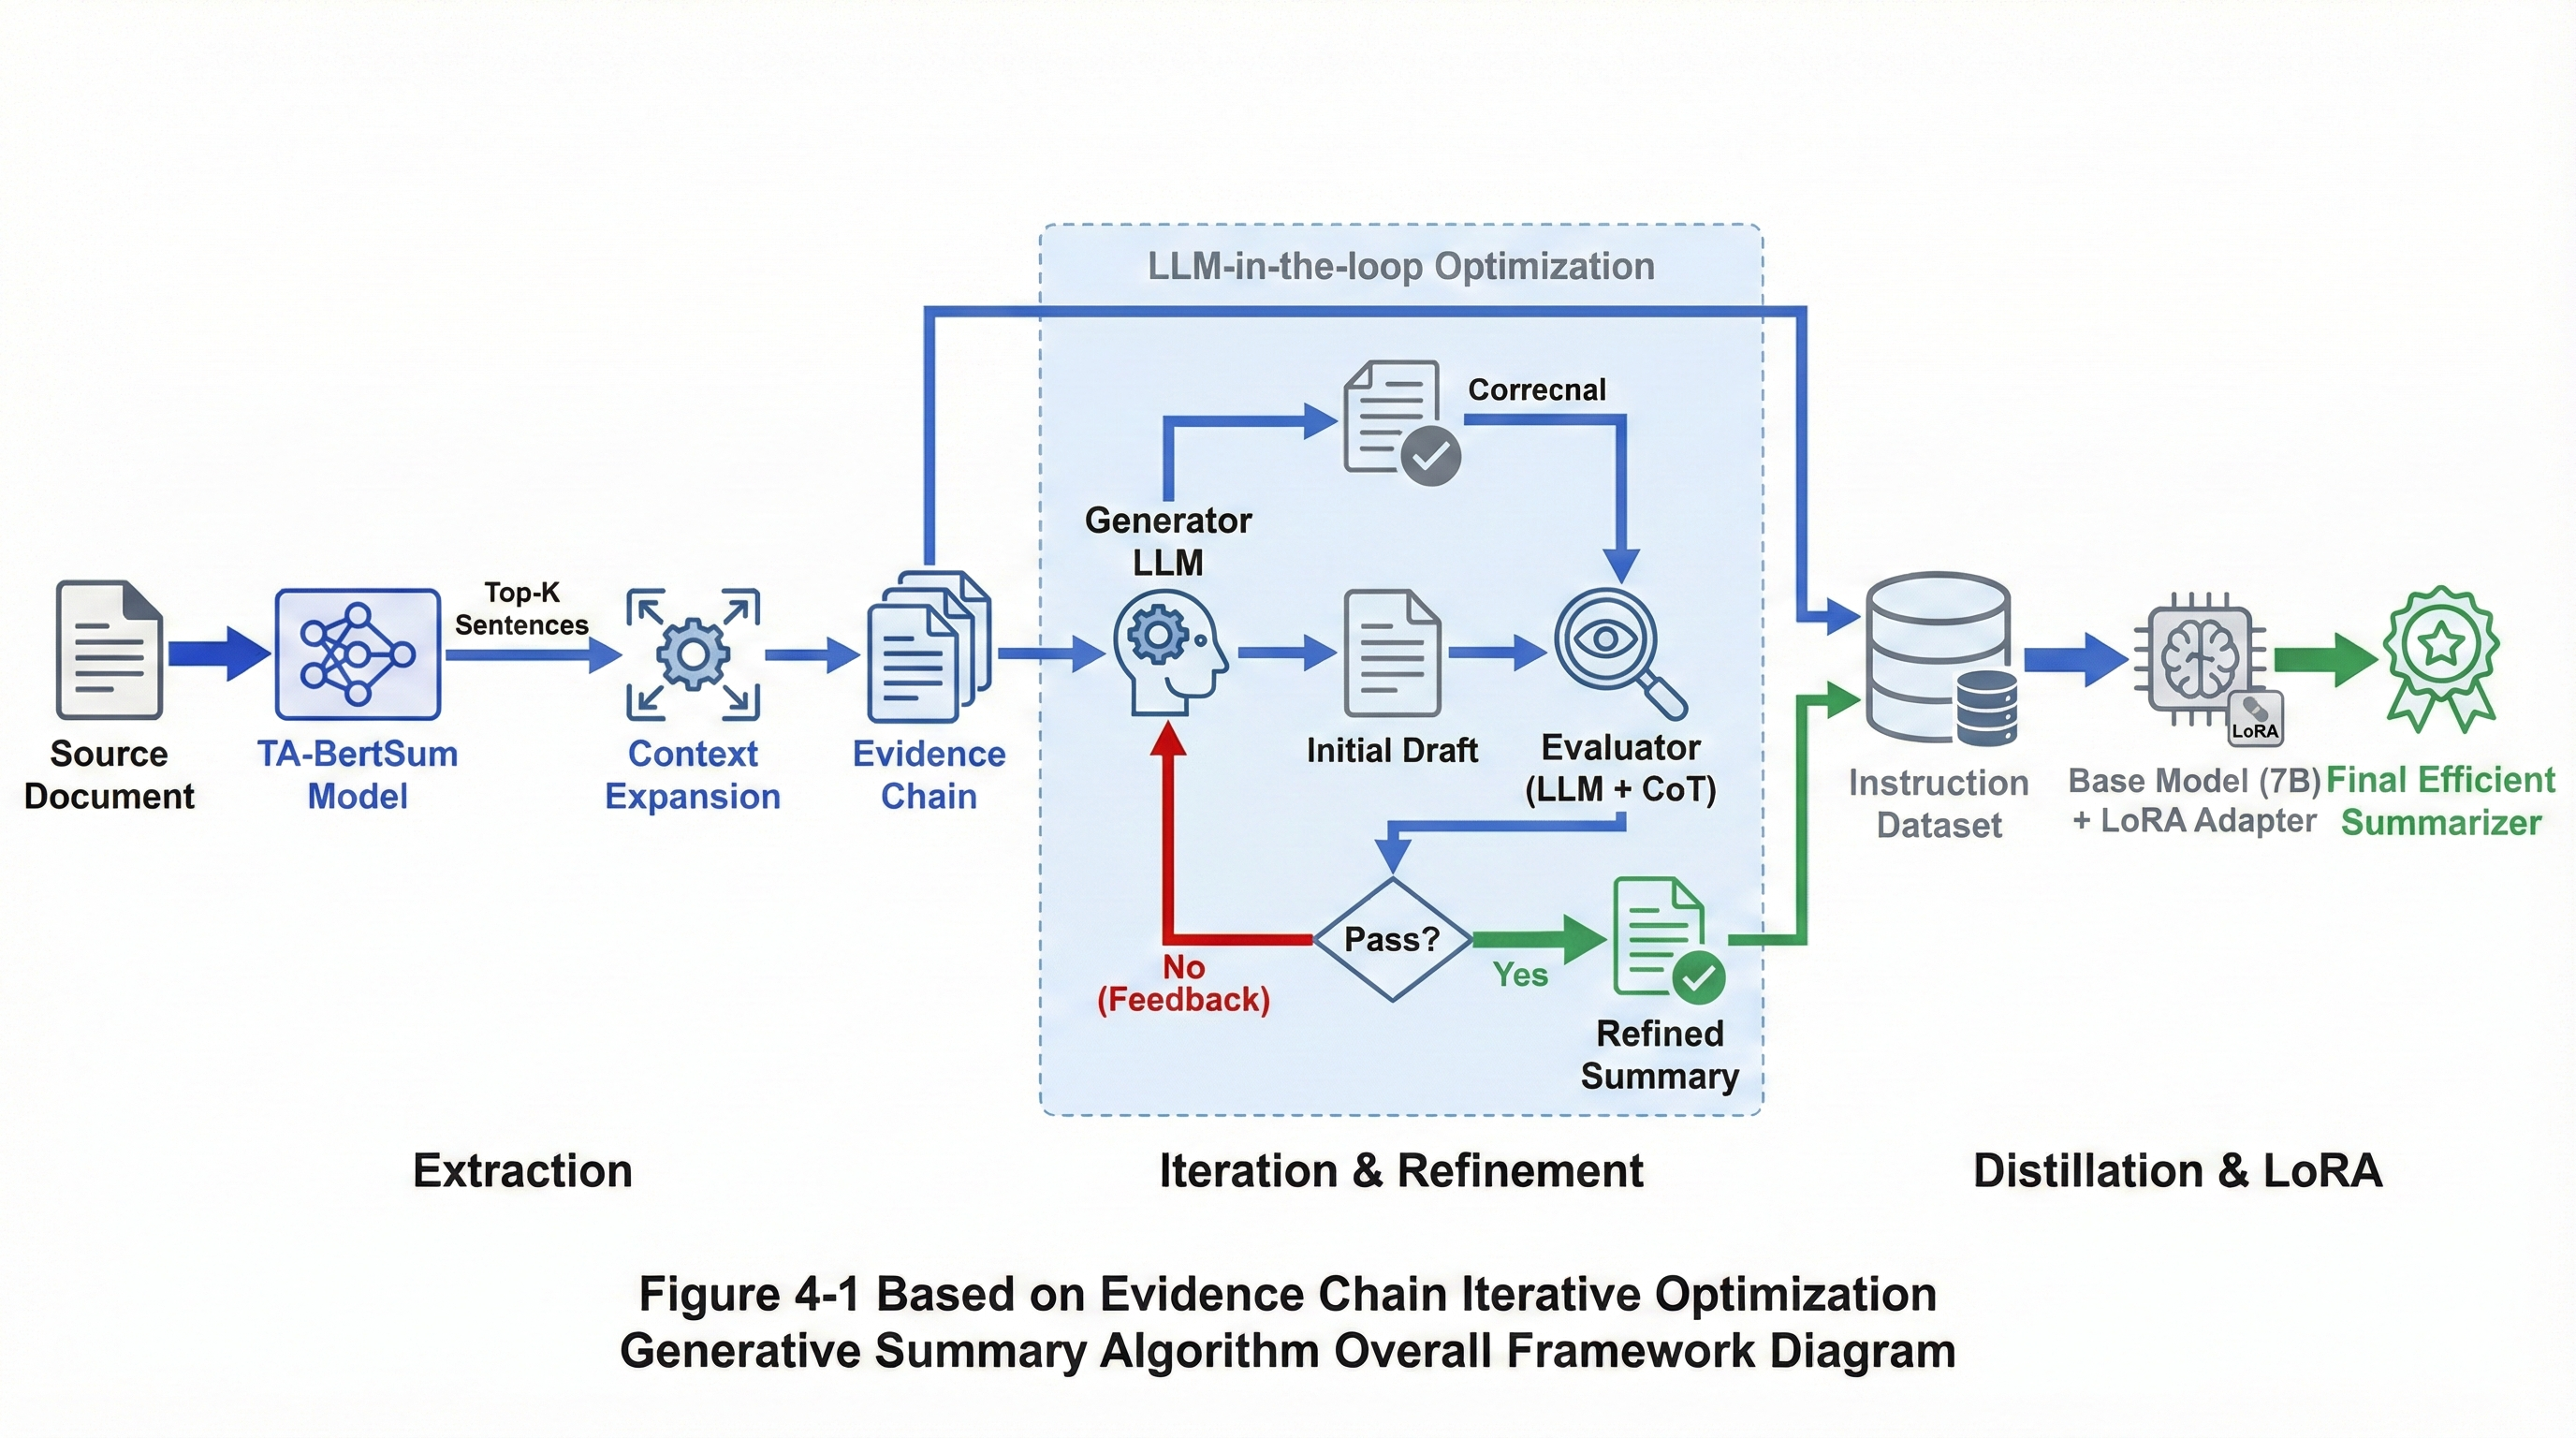
\includegraphics[width=1\textwidth]{figure/chapter5/3.png}
    \caption{首页}
    \label{fig:showfirst}
\end{figure}
%词云展示
%系统架构图
%各个接口的返回信息
\chapter{基于残差金字塔与频谱融合的轻量化图像超分辨率模型}

\section{引言}
图像超分辨率(Image Super-Resolution, SR)指的是从低分辨率(Low-Resolution, LR)输入中重建高分辨率(High-Resolution, HR)图像的过程,这一任务长期以来一直是图像处理领域的基础性研究方向。SR 在众多应用场景中扮演着重要角色,包括医学影像诊断、卫星遥感、视频监控增强以及图像修复等。通过恢复精细的结构细节并改善边缘清晰度,SR 不仅能够提升视觉感知质量,还能增强下游计算机视觉任务(如目标检测、识别和分割)的鲁棒性与性能。

随着 Dong 等人提出 SRCNN~\cite{dong2014learning} 这一开创性工作,深度学习驱动的 SR 研究取得了迅猛进展。特别是在卷积神经网络(Convolutional Neural Networks, CNNs)及其后续的 Transformer 架构的推动下,许多代表性模型(如 RCAN~\cite{zhang2018image}、SwinIR~\cite{liang2021swinir} 和 ELAN~\cite{zhang2022efficient})在图像重建精度与感知质量方面取得了显著成果。这些模型通过引入深层特征层次、注意力机制及高级特征融合策略,在超分任务上实现了优异的重建性能。然而,这类模型通常具有极高的计算复杂度和内存开销,限制了其在移动设备、嵌入式系统和边缘计算平台中的实际部署。

为了解决高复杂度与高参数量带来的挑战,研究者们提出了一系列轻量化 SR 网络结构,致力于在降低计算成本和模型规模的同时保持竞争性的重建性能。其中,一些方法结合了 CNN 与 Transformer 的优势,如 HNCT~\cite{fang2022hybrid} 与 ESRT~\cite{lu2022efficient}。这些模型采用多样的策略,例如集成本地特征提取与全局上下文建模,通过轻量化注意力机制与高效卷积结构来简化计算开销。例如,HNCT 通过高效注意机制降低了 Transformer 模块的计算成本,而 ESRT 则进一步优化了 CNN 与 Transformer 层之间的融合方式。

轻量化 SR 网络的研究意义重大。在低带宽视频传输、移动摄影、实时监控与增强现实(AR)等应用中,模型需以极低功耗和延迟生成高质量帧,从而在资源受限条件下保持感知质量。因此,构建高效的 SR 网络对于提升用户体验与下游任务性能至关重要。

尽管轻量化 SR 研究已取得显著进展,但仍存在若干关键问题亟待解决:  
首先,如何在性能与效率之间实现最佳平衡仍是未解难题。在受限计算预算下,实现细节恢复与全局信息建模的协调至关重要。  
其次,轻量化架构设计需兼顾多尺度空间特征建模能力,以应对不同尺寸与复杂度的图像。许多轻量模型缺乏对多尺度空间关系的刻画,导致在处理纹理复杂或细节丰富的图像时性能受限。  
再次,现有模型往往局限于空间域建模,忽略了频谱域的潜在价值,从而导致高频细节恢复不足、纹理模糊及边缘重建不完整。  
最后,如何在有限计算预算下融合空间域与频谱域信息,实现跨域特征协同增强,仍是高效 SR 模型的研究重点。

为应对上述挑战,本文提出一种结合 CNN 与 Transformer 优势的混合架构——\textbf{RPSFNet (Residual Pyramid and Spectral Fusion Network)},旨在在轻量化条件下实现高效的全局—局部特征建模与频谱增强。RPSFNet 的核心设计思想包括以下几点:

\begin{itemize}
	\item \textbf{残差金字塔块(Residual Pyramid Block, RPB):} 在不同通道组间引入空间移位操作,通过扩张卷积与深度可分离卷积提取多尺度特征,实现细节与结构的高效重建;
	\item \textbf{高效注意力块(Efficient Attention Block, EAB):} 融合门控空间注意单元(Gated Spatial Attention Unit, GSAU),替代传统 MLP 层结构,以降低计算开销并强化特征选择能力;
	\item \textbf{波-傅里叶融合块(Wave-Fourier Fusion Block, WFFB):} 在频域与空间域之间建立双向映射,通过集成小波变换(Wavelet Transform)与傅里叶变换(Fourier Transform)融合多域信息,从而显著增强高频纹理恢复能力;
	\item \textbf{跨层特征协同机制:} 利用浅层卷积捕获低级纹理与边缘特征,深层模块建模长程依赖关系,实现全局上下文与局部细节的协同重建。
\end{itemize}

RPSFNet 采用分层特征提取与频谱融合策略,在轻量化架构中实现高精度重建。通过在空间域与频域之间的特征协同优化,模型在不显著增加参数量的前提下大幅提升了感知质量。实验结果表明,RPSFNet 在多个基准数据集上均取得领先性能,特别是在 Manga109 数据集的 $\times4$ 放大实验中,相较于轻量级模型 IPT-Tiny,PSNR 提升 0.13 dB,且参数量更低,验证了模型在性能与效率之间的优越平衡。

\begin{figure}[H]
	\centering
	\includegraphics[width=0.85\textwidth]{figure/chapter4/f1}
	\caption{RPSFNet 与主流轻量级单图像超分模型在 Manga109 ($\times4$) 数据集上的参数量与 PSNR 对比。}
	\label{fig:rpsf_psnr_param}
\end{figure}

本文的主要贡献可总结如下:
\begin{itemize}
	\item 提出了一种新型轻量化 SR 模型——RPSFNet,该模型结合多尺度空间特征提取、频谱融合与高效长程注意机制,在降低计算复杂度的同时实现了卓越的重建性能;
	\item 设计了波-傅里叶融合模块(WFFB),在空间域与频域间实现信息交互,有效提升了纹理与结构的恢复效果;
	\item 在多个公开基准上验证了 RPSFNet 的优越性能,在保持极低参数量的同时取得了领先的重建精度;
	\item 本文其余部分组织如下:第二节综述轻量化 SR 网络与 Transformer-based 方法;第三节详细介绍 RPSFNet 的总体架构与关键模块;第四节展示实验结果与分析;第五节总结全文并探讨未来研究方向。
\end{itemize}

\section{设计思想及框架}

本章详细介绍所提出的轻量化图像超分辨率网络——\textbf{Residual Pyramid and Spectral Fusion Network (RPSFNet)} 的整体设计思路与核心结构。RPSFNet 的总体目标是在参数量与计算复杂度极低的前提下,实现卓越的超分辨率重建性能。为此,网络通过浅层特征提取、深层金字塔特征提取、频谱融合与图像重建四个阶段,系统性地解决了轻量化 SR 模型中常见的三大问题:局部与全局依赖不足、频域特征缺失以及特征层间融合效率低。

RPSFNet 的总体结构如图~\ref{fig:rpsf_architecture} 所示。模型由三个主要模块构成:浅层特征提取模块(Shallow Feature Extraction Module)、深层特征提取模块(Deep Feature Extraction Module)、以及波–傅里叶融合与重建模块(Wave–Fourier Fusion and Image Reconstruction Module)。每个模块均针对轻量化 SR 网络中的特定挑战进行了结构化设计,旨在平衡性能与计算代价。

\begin{figure}[H]
	\centering
	\includegraphics[width=0.95\textwidth]{figure/chapter4/f2}
	\caption{RPSFNet 的总体框架。模型由多个 RPSF Block 级联而成,每个 Block 包含高效注意力块 (EAB)、门控空间注意单元 (GSAU)、金字塔块 (PB) 以及波–傅里叶融合块 (WFFB)。}
	\label{fig:rpsf_architecture}
\end{figure}

---

\subsection{网络架构}

\paragraph{1) 浅层特征提取}  
浅层特征提取模块旨在从低分辨率输入图像中提取初级纹理与边缘特征。该模块仅包含一个 $3\times3$ 卷积层,将输入图像 $\mathbf{I}_{LR} \in \mathbb{R}^{H\times W\times C_{in}}$ 投影到高维特征空间:
\[
\mathbf{F}_0 = \sigma(\mathrm{Conv}_{3\times3}(\mathbf{I}_{LR})),
\]
其中 $H, W, C_{in}$ 分别表示输入图像的高、宽与通道数,$\sigma(\cdot)$ 为非线性激活函数。所得浅层特征 $\mathbf{F}_0$ 被用作后续深层特征提取模块的输入,以实现从局部到全局的特征递进建模。

\paragraph{2) 深层特征提取}  
为有效捕获多尺度上下文依赖,RPSFNet 堆叠了 $N$ 个 \textbf{残差金字塔与频谱融合块(RPSF Blocks)}。每个块均包含以下三个核心单元:
\begin{itemize}
	\item 高效注意力块(Efficient Attention Block, EAB)
	\item 门控空间注意单元(Gated Spatial Attention Unit, GSAU)
	\item 残差金字塔块(Pyramid Block, PB)
\end{itemize}

RPSF Block 的主要任务是通过特征分层与空间–频谱交互,实现多尺度特征的有效捕获与传递,从而兼顾局部纹理恢复与长程依赖建模。

\paragraph{3) 轻量化 Transformer 模块}  
基于 ESRT~\cite{lu2022efficient} 的轻量 Transformer 模块,本文进一步改进其结构,将传统 MLP 层替换为 \textbf{门控空间注意单元 (GSAU)}。传统 MLP 只能执行线性变换,缺乏空间上下文建模能力,而 GSAU 通过卷积与门控机制联合捕获局部结构信息,从而弥补纯 Transformer 的不足。与标准 MLP 相比,GSAU 模块在以下方面具有优势:
\begin{enumerate}
	\item \textbf{通道扩展(Ghost Expand)}:使用 $1\times1$ 卷积扩展通道数以生成 Ghost 特征图,提高表示能力的同时降低冗余;
	\item \textbf{卷积增强(Convolutional Refinement)}:采用 $7\times7$ 深度可分离卷积增强局部上下文特征;
	\item \textbf{门控机制(Gating Mechanism)}:引入门控控制单元以自适应调节信息流动,从而提升空间依赖建模能力。
\end{enumerate}
这一设计使得 RPSFNet 同时具备 CNN 的局部敏感性与 Transformer 的长程建模优势,在保持轻量化的同时显著提升了全局结构重建能力。

---

\subsection{金字塔块与高效注意力块}

\paragraph{1) 残差金字塔块}  
RPB 是 RPSFNet 的核心结构之一,旨在通过多尺度位移与扩张卷积操作构建自适应的金字塔特征空间。该模块利用不同尺度的 Shift 操作(Shift$_4$、Shift$_8$、Shift$_{16}$)结合扩张卷积提取多尺度上下文信息,具体包括:
\begin{itemize}
	\item $4\times4$ Shift:实现细粒度特征位移,用于捕获局部细节;
	\item $8\times8$ Shift:结合扩张卷积提取中尺度语义信息;
	\item $16\times16$ Shift:通过更大感受野的卷积操作建立全局依赖。
\end{itemize}

该模块的整体处理流程如下:
\[
x_1 = \mathrm{Conv1}(\mathrm{LayerNorm}(x)),
\]
\[
\text{shift}_i = \mathrm{Shift}(\mathrm{DilatedConv}(x_1, r_i)), \quad i \in \{4, 8, 16\},
\]
\[
x_{\text{fused}} = \sum_{i\in\{4,8,16\}} w_i \cdot \text{shift}_i,
\]
\[
x_{\text{out}} = \mathrm{ReLU}(\mathrm{Conv1\times1}(x_{\text{fused}})),
\]
\[
x_{\text{final}} = \mathrm{GSAU}(x_{\text{out}} + x),
\]
其中 $w_i$ 表示可学习的融合权重,用于自适应加权多尺度特征的贡献。通过引入残差连接与门控机制,模块在减少参数与计算开销的同时,增强了特征的表达能力与稳定性。该结构的示意如图~\ref{fig:pyramid_block} 所示。

\begin{figure}[H]
	\centering
	\includegraphics[width=0.9\textwidth]{figure/chapter4/f3}
	\caption{金字塔块(Pyramid Block)的结构。模块通过多尺度移位、深度可分离扩张卷积与门控机制实现多层特征聚合。}
	\label{fig:pyramid_block}
\end{figure}

\paragraph{2) 高效注意力块}  
EAB 模块源自 ESRT 的轻量注意力框架,但进一步进行了结构优化。该模块集成了多头注意力机制(Multi-Head Attention, MHA)与卷积增强机制,能够在低复杂度下实现长程特征依赖建模。通过用 GSAU 替代传统 MLP 层,EAB 显著提升了模型对非线性特征的捕获能力。该结构在性能、可解释性和计算效率之间取得了良好平衡,使得网络在多尺度特征融合阶段更加稳健。

---

\subsection{特征聚合策略}

\paragraph{小波–傅里叶融合模块}  
小波变换(Wavelet Transform)能够有效提取图像中的低频特征(如边缘轮廓),而傅里叶变换(Fourier Transform)则擅长捕获全局频率分布与高频细节。RPSFNet 将两者结合,形成一个双分支结构的频谱融合模块:  
\begin{itemize}
	\item \textbf{Wave 分支:} 使用小波卷积提取低频特征与边缘信息;
	\item \textbf{Fourier 分支:} 通过快速傅里叶变换 (FFT) 将输入特征映射至频率域,并使用逆变换 (IFFT) 重建回空间域;
\end{itemize}

在 Fourier 分支中,输入特征首先经过 FFT 转换为频域表示,再通过卷积层捕获高频成分。随后使用 IFFT 将频域特征还原至空间域,并与 Wave 分支结果在通道维度上融合。此过程融合了空间域、频域和光谱域特征,显著提升了模型的细节恢复能力与信息完备性。

此外,模块在融合阶段采用二维衰减掩膜(two-dimensional decay mask)机制,如图~\ref{fig:wffb_block} 所示。该机制基于曼哈顿距离生成加权矩阵,以增强不同频率分量的显著性,从而实现自适应的频谱注意力分配。整体融合过程不仅保留了空间特征的完整性,还充分利用了频域特征的全局约束特性。

\begin{figure}[H]
	\centering
	\includegraphics[width=0.9\textwidth]{figure/chapter4/f4}
	\caption{波–傅里叶融合模块(WFFB)。模块包含 Wave 与 Fourier 两个分支,后者通过基于曼哈顿距离的衰减掩膜进行加权融合。}
	\label{fig:wffb_block}
\end{figure}

\paragraph{跨域特征融合与重建.}  
在完成空间与频域特征融合后,RPSFNet 通过一个上采样模块生成最终的高分辨率图像。上采样模块基于可学习的反卷积操作与像素重排机制(如 PixelShuffle),实现端到端的分辨率提升。为了保证训练稳定性,输出结果与输入低分辨率图像通过残差连接进行融合,从而进一步提高结构一致性与重建质量。

---

综上,RPSFNet 通过层次化的金字塔特征提取与多域频谱融合策略,实现了在轻量化条件下的高质量超分辨率重建。其核心创新体现在:
\begin{itemize}
	\item 结合了 CNN 的局部建模与 Transformer 的全局建模能力;
	\item 在金字塔结构中引入门控与可学习加权机制以实现多尺度自适应融合;
	\item 通过波–傅里叶融合模块实现空间域与频域的互补增强;
	\item 整体结构具备优异的性能–效率平衡,特别适用于移动端与嵌入式设备的图像增强任务。
\end{itemize}


\section{实验环境设置}
\subsection{数据集介绍}
本文的训练与测试过程基于公开的高质量超分辨率数据集。训练阶段使用 DIV2K 数据集,而测试阶段则选取 Set5、Set14、B100、Urban100 与 Manga109 五个经典基准数据集进行评估。

\textbf{(1)DIV2K 数据集:}
DIV2K(DIVerse 2K resolution)是目前超分辨率任务中最广泛使用的高质量训练集之一,包含 800 张高分辨率图像作为训练集、100 张作为验证集、100 张作为测试集。图像分辨率约为 $2K$($2040\times1080$ 级别),涵盖自然、建筑、人物等多种场景,能够充分提升模型的泛化能力。

\textbf{(2)Set5 数据集:}
Set5 是最早的经典 SR 测试集之一,包含 5 张高分辨率图像,主要为自然场景与人物肖像。虽然规模较小,但其清晰的纹理和边缘细节使其成为衡量 SR 算法性能的重要标准。

\textbf{(3)Set14 数据集:}
Set14 包含 14 张图像,较 Set5 场景更加多样,包括自然景物、动物与城市建筑等。该数据集可验证算法在不同纹理与边缘特征下的鲁棒性。

\textbf{(4)B100 数据集:}
B100 数据集来源于 Berkeley Segmentation Dataset (BSDS300/500) 的子集,共 100 张图像,涵盖大量自然场景与复杂纹理,是测试超分辨率模型在复杂纹理恢复能力上的重要基准。

\textbf{(5)Urban100 数据集:}
Urban100 包含 100 张高分辨率城市建筑场景图像,以其密集的几何结构、重复纹理与精细线条著称,常用于验证模型在恢复建筑结构细节方面的表现。

\textbf{(6)Manga109 数据集:}
Manga109 数据集收录了 109 部日本漫画书的页面,包含超过 20,000 张图像,具有丰富的手绘线条、灰度渐变与高对比边界特征,是检验模型在人工图像和边缘恢复任务中的关键数据集。

\subsection{实验指标介绍}
为了全面评估模型的重建性能,本文采用峰值信噪比(Peak Signal-to-Noise Ratio, PSNR)与结构相似性指数(Structural Similarity Index, SSIM)作为主要的定量评价指标。

\textbf{(1)峰值信噪比 (PSNR):}  
PSNR 衡量重建图像与原始高分辨率图像之间的像素级差异,其定义如下:
\begin{equation}
	\mathrm{PSNR} = 10 \cdot \log_{10} \left( \frac{MAX_I^2}{\mathrm{MSE}} \right)
\end{equation}
其中,$MAX_I$ 表示图像像素的最大可能取值(对于 8-bit 图像通常为 255),$\mathrm{MSE}$ 表示均方误差(Mean Squared Error):
\begin{equation}
	\mathrm{MSE} = \frac{1}{H \times W} \sum_{i=1}^{H}\sum_{j=1}^{W} (I_{ij} - \hat{I}_{ij})^2
\end{equation}
$H$ 与 $W$ 分别表示图像的高度与宽度,$I_{ij}$ 与 $\hat{I}_{ij}$ 分别为原始图像与重建图像在像素位置 $(i,j)$ 的取值。  
PSNR 值越高,说明重建图像与真实图像越接近,失真越小。

\textbf{(2)结构相似性指数 (SSIM):}  
SSIM 从亮度、对比度和结构三个方面衡量两幅图像的相似程度,其定义如下:
\begin{equation}
	\mathrm{SSIM}(x,y) = \frac{(2\mu_x\mu_y + C_1)(2\sigma_{xy} + C_2)}{(\mu_x^2 + \mu_y^2 + C_1)(\sigma_x^2 + \sigma_y^2 + C_2)}
\end{equation}
其中,$\mu_x$ 与 $\mu_y$ 分别表示图像 $x$ 与 $y$ 的平均亮度;$\sigma_x^2$ 与 $\sigma_y^2$ 为方差;$\sigma_{xy}$ 为协方差;$C_1$ 与 $C_2$ 为常数,用于避免分母为零的情况。  
SSIM 的取值范围为 $[0,1]$,值越接近 1 表示两幅图像在结构和感知质量上越一致。

在实际评估中,本文在 YCbCr 色彩空间的 Y 通道上计算 PSNR 与 SSIM,以更准确地反映人眼感知到的亮度质量。

\subsection{实验环境与训练参数设置}

本文提出的方法基于 PyTorch 深度学习框架实现,所有实验均在 NVIDIA A100 80GB PCIe GPU 上进行。  
在训练过程中,我们采用 Adam 优化器,初始学习率设为 $2\times10^{-5}$,并使用 CharbonnierLoss 作为损失函数以增强训练稳定性。  
模型由 4 个 RN(Retentive Network)模块构成,每个模块包含 5 个 Retentive Self-Attention 层、一个通道注意力模块(Channel Attention Module)与一个 SFB 模块(SFB Module),通道数设为 48。  
每次训练批次随机裁剪 $64\times64$ 尺寸的低分辨率(LR)图像块作为输入。  
此外,为确保实验的公平性与可复现性,本文未采用额外的数据增强方法(如 Mixup、RGB 通道随机打乱等)或训练技巧(如预训练与余弦学习率调度等)。

为了验证所提架构的有效性,我们将其与多种先进的轻量化超分辨率(SR)方法进行了比较,分别在放大倍数为 ×2、×3、×4 的情况下进行实验。  
具体而言,我们将本文模型与以下已有工作进行对比:  
EDSR \cite{ref13}、SRMDNF \cite{ref58}、CARN \cite{ref5}、AWSRN-M \cite{ref59}、MADNet \cite{ref60}、SMSR \cite{ref61}、SwinIR \cite{ref4}、ESRT \cite{ref62}、ELAN-light \cite{ref37}、DiVANet \cite{ref6}、SwinIR-NG \cite{ref7} 以及 SCNet \cite{ref63}。  
通过与这些主流方法的系统性比较,我们全面评估了所提出模型在重建质量与模型复杂度之间的性能平衡。

\section{实验结果分析}


\chapter{基于混合注意力的多教师知识蒸馏图像超分辨率模型}

\section{引言}

图像超分辨率(Image Super-Resolution, SR)是计算机视觉领域中的经典问题,其目标是在给定低分辨率图像的情况下,重建出高分辨率的细节结构。
该任务在遥感监测、医学影像、安防视频增强、电子电路识别以及工业缺陷检测等场景中均具有重要的实际应用价值。
近年来,随着深度学习技术的发展,基于神经网络的超分辨率方法取得了显著进展,从最初的卷积神经网络(CNN)到后来的视觉Transformer(ViT)结构,
模型的重建性能持续提升。然而,这一过程中也暴露出一系列核心问题:网络结构日益复杂、参数量剧增、推理成本高昂、以及高频细节恢复能力不足等。
因此,如何在保证重建质量的前提下降低模型复杂度、增强泛化性与细节表达能力,成为当前研究的关键问题。

早期的超分辨率研究主要依赖卷积神经网络,如 SRCNN、VDSR、EDSR 和 RCAN 等经典方法。
这些模型通过逐层卷积提取图像特征,并采用残差学习机制以缓解深层网络训练的梯度消失问题。
其中,RCAN 首次引入了通道注意力机制(Channel Attention),实现了对不同通道特征响应的自适应调节,有效提升了重建精度。
然而,基于卷积的模型在理论上受限于局部感受野,其特征表达能力依赖卷积核堆叠获得。
这种局部卷积特征难以捕捉全局上下文依赖关系,导致模型在恢复长程结构和复杂纹理时表现不足。
同时,为了扩大感受野,研究者往往增加网络深度或宽度,从而导致参数量和计算量的急剧增长,限制了其在资源受限设备上的部署。
此外,传统 CNN 方法对图像的高频信息(如纹理、边缘)恢复能力不足,重建结果容易出现平滑化、纹理缺失等问题,
这在电路图或遥感影像等细节密集场景中尤为明显。

为克服卷积网络的局限性,近年来 Transformer 结构被引入到图像超分辨率任务中。
典型代表如 IPT、SwinIR、Restormer 等模型,利用多头自注意力(Multi-Head Self-Attention, MSA)机制捕获远程依赖关系,
显著提升了全局特征建模能力。
其中,SwinIR 通过滑动窗口(Shifted Window)策略实现了分块自注意力计算,
在保持较高效率的同时实现了局部特征聚合,成为视觉 Transformer 在低层视觉任务中的代表。
然而,这类模型仍然存在三个主要问题:
首先,窗口划分导致窗口间特征交互受限,不同块之间的上下文关联性被削弱,出现结构断裂和特征碎片化;
其次,Transformer 的注意力机制主要在空间域进行,对频域分量(尤其是高频细节)的敏感度不足;
最后,复杂的自注意力计算带来了巨大的算力需求,使得模型难以在轻量化条件下保持高精度表现。
因此,如何在不牺牲性能的前提下降低 Transformer 的计算复杂度,并增强其频域特征建模能力,成为当前亟待解决的核心问题。

另一方面,知识蒸馏(Knowledge Distillation, KD)被广泛应用于模型压缩与性能提升中。
其基本思想是通过教师模型(Teacher)向学生模型(Student)传递知识,
使学生模型在保持低复杂度的同时获得接近教师模型的性能表现。
在超分辨率领域,研究者提出了多种蒸馏策略,如特征蒸馏、响应蒸馏和感知蒸馏等。
例如,SRKD 通过在特征空间上约束学生与教师的一致性,提高了学生模型的结构还原能力;
DKD-SR 则在特征分布层面引入对齐损失,强化了学生的特征表征。
然而,传统的知识蒸馏方法大多采用单一教师模型,这种单源蒸馏在实践中存在明显局限:
教师模型的特征分布通常具有结构偏向,若教师模型对某类纹理或模式建模不充分,
学生模型在对应场景下也会继承这种偏差,造成泛化性能下降。
此外,单教师蒸馏的知识多样性不足,难以涵盖多种尺度、频率和结构特征;
同时,传统蒸馏往往仅在最终输出层施加监督,忽略了中间层语义层次的知识迁移。
这些问题使得学生模型难以在不同图像类型间稳定泛化。

针对上述问题,本章引入了多教师知识蒸馏(Multi-Teacher Knowledge Distillation, MTKD)策略,
通过融合多个结构互补的教师模型,使学生网络在训练过程中同时学习不同模型的特征归纳能力。
具体而言,本章选择 EDSR、RCAN 和 SwinIR 作为教师模型:EDSR 具有良好的结构还原能力,
RCAN 擅长通道特征选择,而 SwinIR 善于捕获全局依赖信息。
这种多教师协同指导方式可以在特征空间中形成互补约束,
学生网络在学习过程中不仅继承了单个教师的优势特征,还获得了跨结构的泛化能力。
此外,本章设计了特征级别的自适应加权融合机制,
在不同教师输出的特征映射间引入动态权重,从而避免了多源知识冲突问题。

除了知识蒸馏策略外,本章还从结构层面提出了一种结合频域增强与混合注意力机制的高效 Transformer 网络,
即 Hybrid Attention DCT Transformer(HADCT)。
与传统的 SwinIR 或 Restormer 不同,HADCT 在窗口注意力模块中引入了离散余弦变换(Discrete Cosine Transform, DCT),
使网络能够在局部窗口内直接建模频域能量分布。
这一设计使得模型不仅能够在空间域捕获纹理与结构信息,
还能够在频域上聚焦高频成分,从而提升细节恢复能力。
同时,为解决窗口注意力存在的边界断裂与上下文割裂问题,HADCT 设计了重叠跨窗口注意力模块(Overlapping Cross-Attention Block, OCAB),
在窗口边缘区域引入重叠机制,实现跨窗口信息交互。
此外,模型中还嵌入了卷积通道注意力(CAB)模块,以增强特征选择性并引入局部非线性表达。
通过多层残差混合注意力组(Residual Hybrid Attention Group, RHAG)的堆叠,
模型在不同尺度下实现了全局与局部特征的层次化融合,显著提升了重建质量。

总体而言,本章提出的 HADCT 网络在结构设计与训练策略上均具有创新性。
在结构层面,它通过频域增强与混合注意力协同机制,实现了高频信息重建与全局特征捕获的统一;
在训练机制上,通过多教师知识蒸馏引入多源语义约束,显著提升了学生模型的泛化性能与稳健性。
与传统的单教师卷积蒸馏方法相比,本章方法能够在更低的参数量与计算成本下,
达到接近甚至超过大型 Transformer 模型的重建性能。

本文方法的主要创新点可总结如下:
(1)提出了一种结合频域增强与混合注意力机制的 Transformer 框架,
在窗口注意力中引入 DCT/IDCT 操作,显式建模高频分量,提高细节恢复质量;
(2)设计了跨窗口重叠注意力模块(OCAB),实现窗口间的特征连续与上下文融合;
(3)构建了多教师知识蒸馏体系,通过 EDSR、RCAN 和 SwinIR 的特征融合指导,
使学生网络在不同结构特征间自适应学习;
(4)在复杂度控制方面,模型采用轻量化通道压缩与残差连接结构,
在 $256\times256$ 输入下参数量约 9.4M、FLOPs 约 $1.38\times10^{10}$,在保证重建性能的同时具备良好的部署效率。

本章的研究目标是建立一个兼顾性能、复杂度与可解释性的统一超分辨率框架。
通过在 Transformer 框架中引入 DCT 频域建模与多教师蒸馏策略,
本文方法有效融合了空间、频率与语义三类特征信息,
为后续轻量化超分辨率模型的研究提供了新的思路。
接下来的章节将详细介绍 HADCT 网络的整体设计思路、关键模块结构、蒸馏机制以及实验验证结果。


\section{设计思路及框架}

\subsection{网络架构}

本章提出的 Hybrid Attention DCT Transformer(HADCT)是一种融合空间域与频域特征的多层超分辨率生成网络。
其总体结构如图~\ref{fig:hadct-framework} 所示,主要由三个部分组成:
浅层特征提取模块、深层残差频域注意力组(Residual Frequency-Attention Group, RFAG)模块,以及重建模块。
整个模型以残差学习为核心思想,通过多级频域注意力交互实现全局—局部—频率的协同建模。

输入低分辨率图像 $\mathbf{I}_{\mathrm{LR}} \in \mathbb{R}^{3\times H\times W}$ 经 PixelUnshuffle 操作重排为 $r^2$ 个通道:
\begin{equation}
	\mathbf{X}_0 = \mathrm{PixelUnshuffle}(\mathbf{I}_{\mathrm{LR}}),
\end{equation}
其中 $r$ 为上采样倍率(例如 $r=4$ 时,输入通道数为 $3\times16$)。
随后经卷积层提取初始浅层特征:
\begin{equation}
	\mathbf{F}_0 = \sigma(\mathrm{Conv}_{3\times3}(\mathbf{X}_0)),
\end{equation}
其中 $\sigma(\cdot)$ 表示激活函数(GELU)。

浅层特征 $\mathbf{F}_0$ 被输入至 $N$ 个残差频域注意力组(RFAG)。
每个 RFAG 内部由若干频域增强注意力块(FAAB)与一个频域重叠注意力块(FOAB)组成。
该过程可形式化为:
\begin{equation}
	\mathbf{F}_N = \mathcal{R}_N(\mathcal{R}_{N-1}(\cdots \mathcal{R}_1(\mathbf{F}_0))),
\end{equation}
其中 $\mathcal{R}_i(\cdot)$ 表示第 $i$ 个 RFAG 的映射函数。

RFAG 输出经卷积层与残差相加形成深层特征:
\begin{equation}
	\mathbf{F}_{\mathrm{deep}} = \mathrm{Conv}_{3\times3}(\mathbf{F}_N) + \mathbf{F}_0.
\end{equation}

最终通过上采样重建模块生成高分辨率图像:
\begin{equation}
	\mathbf{I}_{\mathrm{SR}} = \mathcal{U}(\mathbf{F}_{\mathrm{deep}}),
\end{equation}
其中 $\mathcal{U}(\cdot)$ 表示 PixelShuffle 与卷积操作的组合:
\begin{equation}
	\mathcal{U}(\mathbf{F}) = \mathrm{Conv}_{3\times3}(\mathrm{PixelShuffle}_r(\mathrm{Conv}_{3\times3}(\mathbf{F}))).
\end{equation}

通过这种端到端结构,HADCT 同时利用卷积的局部特征提取优势与 Transformer 的全局建模能力,
并在频域上显式建模高频成分,实现多域特征的高效融合。

\begin{figure}[h]
	\centering
	\includegraphics[width=0.96\linewidth]{figure/chapter5/f1}
	\caption{HADCT 网络总体结构框图。网络包含浅层特征提取、多个残差频域注意力组(RFAG)及上采样重建模块。RFAG 内部由频域增强注意力块(FAAB)与频域重叠注意力块(FOAB)构成,用于实现局部-全局-频率特征融合。}
	\label{fig:hadct-framework}
\end{figure}

\subsection{频域增强注意力块}

频域增强注意力块(Frequency-Augmented Attention Block, FAAB)是 HADCT 的核心单元之一,
通过在窗口注意力中引入 DCT/IDCT 操作,使注意力机制在频域中执行,以显式强化高频细节建模能力。
其内部结构如图~\ref{fig:faab-arch} 所示。

设输入特征为 $\mathbf{X}\in\mathbb{R}^{B\times H\times W\times C}$,
FAAB 包含三条主要分支:频域注意力分支、局部卷积分支和通道注意力分支。

首先,对输入进行层归一化:
\begin{equation}
	\hat{\mathbf{X}} = \mathrm{LN}(\mathbf{X}),
\end{equation}
然后执行窗口划分 $\{\mathbf{X}_i\}$:
\begin{equation}
	\mathbf{X}_i \in \mathbb{R}^{B\times W\times W\times C}, \quad i=1,\dots,M,
\end{equation}
其中 $M$ 为窗口数量。  
每个窗口通过二维 DCT 转换至频域:
\begin{equation}
	\mathbf{X}_i^{\mathrm{DCT}} = \mathcal{D}(\mathbf{X}_i),
\end{equation}
在频域上执行多头自注意力(MSA):
\begin{equation}
	\mathbf{Z}_i^{\mathrm{DCT}} = \mathrm{MSA}_{\mathrm{freq}}(\mathbf{X}_i^{\mathrm{DCT}}),
\end{equation}
并通过逆变换得到增强特征:
\begin{equation}
	\mathbf{Z}_{\mathrm{attn}} = \mathcal{D}^{-1}(\mathbf{Z}_i^{\mathrm{DCT}}).
\end{equation}

局部卷积分支利用两个 $3\times3$ 卷积层与 GELU 激活提取空间特征:
\begin{equation}
	\mathbf{Z}_{\mathrm{conv}} = \mathrm{Conv}_{3\times3}(\mathrm{GELU}(\mathrm{Conv}_{3\times3}(\mathbf{X}))).
\end{equation}

通道注意力分支(CAB)用于建模通道间相关性:
\begin{equation}
	\mathbf{Z}_{\mathrm{ch}} = \sigma(W_2\delta(W_1\mathrm{GAP}(\mathbf{Z}_{\mathrm{conv}})))\odot \mathbf{Z}_{\mathrm{conv}},
\end{equation}
其中 $\mathrm{GAP}$ 为全局平均池化,$\delta$ 为 ReLU,$\sigma$ 为 Sigmoid。

三分支融合采用加权残差形式:
\begin{equation}
	\mathbf{Y} = \mathbf{X} + \mathrm{DropPath}(\mathbf{Z}_{\mathrm{attn}}) + \gamma \mathbf{Z}_{\mathrm{ch}},
\end{equation}
其中 $\gamma$ 为可学习比例系数。
最终经 MLP 实现非线性映射:
\begin{equation}
	\mathbf{Y} = \mathbf{Y} + \mathrm{DropPath}(\mathrm{MLP}(\mathrm{LN}(\mathbf{Y}))).
\end{equation}

\begin{figure}[h]
	\centering
	\includegraphics[width=0.9\linewidth]{figure/chapter5/f2}
	\caption{频域增强注意力块(FAAB)结构。模块在窗口内执行 DCT/IDCT 操作,
		将注意力显式迁移至频域,实现高频增强与通道特征协同。}
	\label{fig:faab-arch}
\end{figure}


\subsection{频域重叠注意力块}

为解决窗口分块导致的边界信息割裂问题,HADCT 设计了频域重叠注意力块(Frequency Overlapping Attention Block, FOAB)。
其思想是在计算注意力时,扩展键/值窗口的范围以包含邻域重叠区域,实现跨窗口的频域特征交互。
结构如图~\ref{fig:foab-arch} 所示。

设原始窗口大小为 $W$,扩展后为 $W' = W + \Delta$,
FOAB 的核心注意力公式为:
\begin{equation}
	\mathrm{Attn}_{\mathrm{FOA}} = \mathrm{Softmax}\!\left(\frac{\mathbf{Q}\mathbf{K}_{\mathrm{ext}}^\top}{\sqrt{d}} + \mathbf{B}_{W,W'}\right)\mathbf{V}_{\mathrm{ext}},
\end{equation}
其中 $\mathbf{K}_{\mathrm{ext}}$ 与 $\mathbf{V}_{\mathrm{ext}}$ 分别为扩展窗口的键和值,
$\mathbf{B}_{W,W'}$ 为相对位置偏置。
通过扩展窗口的频域交互,模型在边界区域获得更连续的上下文信息,
有效提升了电路纹理、线条等结构的连续性和稳定性。

\begin{figure}[h]
	\centering
	\includegraphics[width=0.9\linewidth]{figure/chapter5/f3}
	\caption{频域重叠注意力块(FOAB)结构。FOAB 扩展键值窗口范围,在频域实现跨窗口特征交互与边界连续性增强。}
	\label{fig:foab-arch}
\end{figure}


\subsection{残差频域注意力组}

残差频域注意力组(Residual Frequency-Attention Group, RFAG)是整个 HADCT 的核心结构单元,
通过多层 FAAB 与一个 FOAB 组成复合残差路径,以实现多层特征聚合。
其数学表达为:
\begin{equation}
	\mathbf{Y} = \mathcal{F}_{\mathrm{FOAB}}(\mathcal{F}_{\mathrm{FAAB}}^{(L)}(\mathbf{X})) + \mathbf{X},
\end{equation}
其中 $L$ 为组内 FAAB 数量。
为了稳定训练并防止梯度爆炸,RFAG 引入了 DropPath 随机残差机制:
\begin{equation}
	\mathbf{Y} = \mathbf{X} + \mathrm{DropPath}(\mathcal{F}_{\mathrm{FOAB}}(\cdot)) + \mathrm{DropPath}(\mathcal{F}_{\mathrm{FAAB}}(\cdot)).
\end{equation}
这种分层残差设计使得模型能够在高层保持全局一致性,同时在底层捕获丰富的高频结构特征。


\subsection{多教师知识蒸馏机制}

为进一步提升模型泛化能力与特征鲁棒性,HADCT 在训练阶段引入多教师知识蒸馏策略。
设有三种教师模型 $\{\mathcal{T}_1, \mathcal{T}_2, \mathcal{T}_3\}$,分别对应 EDSR、RCAN 与 SwinIR,
分别强调结构还原、通道建模与全局依赖捕获能力。

给定输入 $\mathbf{I}_{\mathrm{LR}}$,教师模型产生特征输出:
\begin{equation}
	\mathbf{F}_{T_i} = \mathcal{T}_i(\mathbf{I}_{\mathrm{LR}}), \quad i\in\{1,2,3\}.
\end{equation}
学生模型将三者融合为:
\begin{equation}
	\mathbf{F}_{\mathrm{MT}} = \sum_{i=1}^{3}\alpha_i\mathbf{F}_{T_i}, \quad \sum_i\alpha_i=1.
\end{equation}
融合特征输入学生网络:
\begin{equation}
	\mathbf{I}_{\mathrm{SR}} = \mathcal{S}(\mathbf{F}_{\mathrm{MT}}; \Theta_{\mathrm{Stu}}).
\end{equation}
多教师蒸馏损失定义为:
\begin{equation}
	\mathcal{L}_{\mathrm{KD}} = \sum_i\lambda_i\|\mathbf{F}_{\mathrm{Stu}}-\mathbf{F}_{T_i}\|_1 + \mu\,\mathrm{KL}(p_{\mathrm{Stu}}\|p_{T_i}),
\end{equation}
其中 $\lambda_i$ 和 $\mu$ 为权重参数。


\subsection{损失函数与优化目标}

HADCT 的最终训练目标由像素重建损失、感知损失与蒸馏损失共同组成:
\begin{equation}
	\mathcal{L}_{\mathrm{total}} = \lambda_1\mathcal{L}_{\mathrm{pix}} + \lambda_2\mathcal{L}_{\mathrm{percep}} + \lambda_3\mathcal{L}_{\mathrm{KD}},
\end{equation}
其中:
\begin{align}
	\mathcal{L}_{\mathrm{pix}} &= \|\mathbf{I}_{\mathrm{SR}} - \mathbf{I}_{\mathrm{HR}}\|_1, \\
	\mathcal{L}_{\mathrm{percep}} &= \|\phi(\mathbf{I}_{\mathrm{SR}}) - \phi(\mathbf{I}_{\mathrm{HR}})\|_2^2,
\end{align}
$\phi(\cdot)$ 表示由 VGG 网络提取的感知特征。
优化器采用 AdamW,并通过余弦退火(Cosine Annealing)策略动态调整学习率。

综上所述,HADCT 通过引入频域增强机制(FAAB)、跨窗口特征交互(FOAB)以及残差层级聚合(RFAG),
实现了空间、通道与频率三维特征的协同优化。
结合多教师知识蒸馏策略,模型在轻量化与性能之间取得了优雅的平衡,
为复杂结构(如电路图与工程图)中的高频细节超分辨提供了新的解决路径。




\section{实验环境设置}
\subsection{数据集介绍}
本文的训练与测试过程基于公开的高质量超分辨率数据集。训练阶段使用 DIV2K 数据集,而测试阶段则选取 Set5、Set14、B100、Urban100 与 Manga109 五个经典基准数据集进行评估。

\textbf{(1)DIV2K 数据集:}
DIV2K(DIVerse 2K resolution)是目前超分辨率任务中最广泛使用的高质量训练集之一,包含 800 张高分辨率图像作为训练集、100 张作为验证集、100 张作为测试集。图像分辨率约为 $2K$($2040\times1080$ 级别),涵盖自然、建筑、人物等多种场景,能够充分提升模型的泛化能力。

\textbf{(2)Set5 数据集:}
Set5 是最早的经典 SR 测试集之一,包含 5 张高分辨率图像,主要为自然场景与人物肖像。虽然规模较小,但其清晰的纹理和边缘细节使其成为衡量 SR 算法性能的重要标准。

\textbf{(3)Set14 数据集:}
Set14 包含 14 张图像,较 Set5 场景更加多样,包括自然景物、动物与城市建筑等。该数据集可验证算法在不同纹理与边缘特征下的鲁棒性。

\textbf{(4)B100 数据集:}
B100 数据集来源于 Berkeley Segmentation Dataset (BSDS300/500) 的子集,共 100 张图像,涵盖大量自然场景与复杂纹理,是测试超分辨率模型在复杂纹理恢复能力上的重要基准。

\textbf{(5)Urban100 数据集:}
Urban100 包含 100 张高分辨率城市建筑场景图像,以其密集的几何结构、重复纹理与精细线条著称,常用于验证模型在恢复建筑结构细节方面的表现。

\textbf{(6)Manga109 数据集:}
Manga109 数据集收录了 109 部日本漫画书的页面,包含超过 20,000 张图像,具有丰富的手绘线条、灰度渐变与高对比边界特征,是检验模型在人工图像和边缘恢复任务中的关键数据集。

\subsection{实验指标介绍}
为了全面评估模型的重建性能,本文采用峰值信噪比(Peak Signal-to-Noise Ratio, PSNR)与结构相似性指数(Structural Similarity Index, SSIM)作为主要的定量评价指标。

\textbf{(1)峰值信噪比 (PSNR):}  
PSNR 衡量重建图像与原始高分辨率图像之间的像素级差异,其定义如下:
\begin{equation}
	\mathrm{PSNR} = 10 \cdot \log_{10} \left( \frac{MAX_I^2}{\mathrm{MSE}} \right)
\end{equation}
其中,$MAX_I$ 表示图像像素的最大可能取值(对于 8-bit 图像通常为 255),$\mathrm{MSE}$ 表示均方误差(Mean Squared Error):
\begin{equation}
	\mathrm{MSE} = \frac{1}{H \times W} \sum_{i=1}^{H}\sum_{j=1}^{W} (I_{ij} - \hat{I}_{ij})^2
\end{equation}
$H$ 与 $W$ 分别表示图像的高度与宽度,$I_{ij}$ 与 $\hat{I}_{ij}$ 分别为原始图像与重建图像在像素位置 $(i,j)$ 的取值。  
PSNR 值越高,说明重建图像与真实图像越接近,失真越小。

\textbf{(2)结构相似性指数 (SSIM):}  
SSIM 从亮度、对比度和结构三个方面衡量两幅图像的相似程度,其定义如下:
\begin{equation}
	\mathrm{SSIM}(x,y) = \frac{(2\mu_x\mu_y + C_1)(2\sigma_{xy} + C_2)}{(\mu_x^2 + \mu_y^2 + C_1)(\sigma_x^2 + \sigma_y^2 + C_2)}
\end{equation}
其中,$\mu_x$ 与 $\mu_y$ 分别表示图像 $x$ 与 $y$ 的平均亮度;$\sigma_x^2$ 与 $\sigma_y^2$ 为方差;$\sigma_{xy}$ 为协方差;$C_1$ 与 $C_2$ 为常数,用于避免分母为零的情况。  
SSIM 的取值范围为 $[0,1]$,值越接近 1 表示两幅图像在结构和感知质量上越一致。

在实际评估中,本文在 YCbCr 色彩空间的 Y 通道上计算 PSNR 与 SSIM,以更准确地反映人眼感知到的亮度质量。

\subsection{实验环境与训练参数设置}

本文提出的方法基于 PyTorch 深度学习框架实现,所有实验均在 NVIDIA A100 80GB PCIe GPU 上进行。  
在训练过程中,我们采用 Adam 优化器,初始学习率设为 $2\times10^{-5}$,并使用 CharbonnierLoss 作为损失函数以增强训练稳定性。  
模型由 4 个 RN(Retentive Network)模块构成,每个模块包含 5 个 Retentive Self-Attention 层、一个通道注意力模块(Channel Attention Module)与一个 SFB 模块(SFB Module),通道数设为 48。  
每次训练批次随机裁剪 $64\times64$ 尺寸的低分辨率(LR)图像块作为输入。  
此外,为确保实验的公平性与可复现性,本文未采用额外的数据增强方法(如 Mixup、RGB 通道随机打乱等)或训练技巧(如预训练与余弦学习率调度等)。

为了评估所提出的MTKD方法的有效性,我们遵循[78]中的评估实践,选择了广泛使用的基于CNN的ISR模型:EDSR[40],以及一种流行的基于Transformer的模型:SwinIR[39]进行比较。它们的开源完整原始模型在这里被用作教师网络。由于本文的目的是开发和验证一种新的知识蒸馏方法,而不是设计一种新颖的轻量级模型,我们采用这些教师网络的现有低复杂度变体作为紧凑的学生模型。对于EDSR和SwinIR,学生模型与其原始论文中的相同:EDSR-baseline[40]和SwinIR-lightweight[39]。这些教师和学生模型的配置细节总结在表1中。为了全面评估ISR性能,我们针对多个尺度因子(包括×2、×3和×4)的SR任务训练和评估了每个模型。

\section{实验结果分析}
\subsection{定量结果分析}

\chapter{总结与展望}


\end{document}
